%% 
%% Copyright 2007-2019 Elsevier Ltd
%% 
%% This file is part of the 'Elsarticle Bundle'.
%% ---------------------------------------------
%% 
%% It may be distributed under the conditions of the LaTeX Project Public
%% License, either version 1.2 of this license or (at your option) any
%% later version.  The latest version of this license is in
%%    http://www.latex-project.org/lppl.txt
%% and version 1.2 or later is part of all distributions of LaTeX
%% version 1999/12/01 or later.
%% 
%% The list of all files belonging to the 'Elsarticle Bundle' is
%% given in the file `manifest.txt'.
%% 
%% Template article for Elsevier's document class `elsarticle'
%% with harvard style bibliographic references

\documentclass[preprint,12pt,authoryear]{elsarticle}

%% Use the option review to obtain double line spacing
%% \documentclass[authoryear,preprint,review,12pt]{elsarticle}

%% Use the options 1p,twocolumn; 3p; 3p,twocolumn; 5p; or 5p,twocolumn
%% for a journal layout:
%% \documentclass[final,1p,times,authoryear]{elsarticle}
%% \documentclass[final,1p,times,twocolumn,authoryear]{elsarticle}
%% \documentclass[final,3p,times,authoryear]{elsarticle}
%% \documentclass[final,3p,times,twocolumn,authoryear]{elsarticle}
%% \documentclass[final,5p,times,authoryear]{elsarticle}
%% \documentclass[final,5p,times,twocolumn,authoryear]{elsarticle}

%% For including figures, graphicx.sty has been loaded in
%% elsarticle.cls. If you prefer to use the old commands
%% please give \usepackage{epsfig}

%% The amssymb package provides various useful mathematical symbols
\usepackage{amssymb}
%% The amsthm package provides extended theorem environments
\usepackage{amsthm}
% package added by zhixuan
\usepackage{amsmath}
\usepackage{float}

%% The lineno packages adds line numbers. Start line numbering with
%% \begin{linenumbers}, end it with \end{linenumbers}. Or switch it on
%% for the whole article with \linenumbers.
%% \usepackage{lineno}

\journal{Computer Methods in Applied Mechanics and Engineering}
\begin{document}
\begin{frontmatter}
\title{A Random Choice SPH Scheme with Adaptive Viscosity}
%\tnotetext[mytitlenote]{Can add  title note here}
%% Group authors per affiliation:
\author{Zhixuan Cao}
\ead{zhixuan.cao@ansys.com}
\address{Fluids Business Unit, Ansys Inc., Lebanon, NH, 03766, USA}
\author{Abani Patra \fnref{mycorrespondingauthor}}
\ead{abani.patra@tufts.edu}
\address{Department of Computer Science and Department of Mathematics, Tufts University, Medford, MA, 02153, USA}
\author{E. Bruce Pitman}
\ead{pitman@buffalo.edu}
\address{Department of Materials Design and Innovation, The State University of New York at Buffalo, Amherst, NY, 14260, USA}
%\fntext[myfootnote]{Since 1880.}
%% or include affiliations in footnotes:
%\author[mymainaddress,mysecondaryaddress]%{Elsevier Inc}
%\ead[url]{www.elsevier.com}
%\author[mysecondaryaddress]{Global Customer Service\corref{mycorrespondingauthor}}
\cortext[mycorrespondingauthor]{Corresponding author}
%\cortext[mycorrespondingauthor]{abani@buffalo.edu}
%\ead{abani@buffalo.edu}
%\address[mymainaddress]{1600 John F Kennedy Boulevard, Philadelphia}
%\address[mysecondaryaddress]{360 Park Avenue South, New York}

\begin{abstract}
Implementation of the classical smoothed particle hydrodynamics (SPH) method in high-speed compressible flow employs explicit artificial viscosity to properly capture shock waves. The amount of artificial viscosity introduced in this explicit way depends on coefficients of the artificial viscosity term.
We propose a novel SPH scheme that combines an approximate version of Glimm\rq{}s Random Choice method (RCM) with SPH. RCM properly resolves and then samples all hydrodynamic waves. Our version approximately resolves hydrodynamic waves, and samples the approximate solution. The new scheme does not require explicit artificial viscosity term.
We test this method on standard one dimensional shock tube problems and observe several attractive features. This method introduces adaptive artificial viscosity, assigning larger dissipation around discontinuities and smaller elsewhere.  Less smearing of discontinuity is introduced by this method in one dimensional shock tube tests. In addition, it also helps ameliorate pressure ``wiggle" around contact discontinuity. When applied to three dimensional jet flow, this method is demonstrated to introduce less overall-dissipation.
%Our ultimate goal is to apply this method to jet flow. Because of the high shear rate in this application, we introduce a highly tuned eddy viscosity that is applied only near the shear surface. The combination of the SPH and RCM together with a shear viscosity produces nicely resolved jet profiles.

\end{abstract}
\begin{keyword}
Smoothed Particle Hydrodynamics (SPH), Random Choice Method (RCM), Riemann Solver, Artificial viscosity, Hyperbolic PDEs
\end{keyword}
\end{frontmatter}

\section{Introduction}
Smoothed particle hydrodynamics (SPH) \citep{gingold1977smoothed,lucy1977numerical} is a mesh-free particle method based on a Lagrangian formulation of the governing equations of motion.
SPH has been widely applied to different areas in engineering and science. As should be expected, SPH possesses certain advantages and certain disadvantages relative to finite difference and finite element solvers. Principally, as a Lagrangian solver, SPH conserves mass exactly. 
In addition, because of its formulation SPH automatically concentrates numerical effort in regions of high density and adapts to arbitrary geometries. On the other hand, 
SPH has difficulty capturing shock waves and contact discontinuities. To overcome numerical oscillations at discontinuities, classical SPH introduces an artificial viscosity term. As it is most often used, when two SPH particles are approaching, a von Neumann type viscosity is introduced
\citep{monaghan1983shock, monaghan1997sph,klapp2012strong}. 
Various methods have been introduced to tune the artificial viscosity, turning it on and off for particular wave features. However, tuning switches cannot properly accommodate every kind of wave that might arise, and spurious effects and unphysical damping persist (see, for example, \cite{borgani2012hydrodynamic,flebbe1994smoothed,morris1997switch, dolag2005turbulent,cullen2010inviscid,sigalotti2008adaptive,puri2014comparison}).
 
To overcome troublesome oscillations, \citet{inutsuka2002reformulation} and later \citet{cha2003implementations} formulated an SPH scheme that uses Riemann problems to resolve the interactions of particles. This Godunov-SPH (GSPH) method can resolve shocks and pressure oscillations without additional artificial viscosity \citep{inutsuka2002reformulation, cha2003implementations,iwasaki2011smoothed, puri2014approximate,borgani2012hydrodynamic}. It has also been shown to introduce less damping in turbulent mixing \citep{cha2010kelvin, borgani2012hydrodynamic} than standard SPH. 
However, the dissipation introduced by GSPH is still larger than physically relevant, to the point
of inhibiting the development of the Kelvin-Helmholtz instability under certain conditions \citep{borgani2012hydrodynamic}.

The Godunov approach to solving Riemann problems in the context of numerical methods for conservation laws is to integrate the Riemann problem solution over a spatial interval of interest. A different approach is given by the random choice method (RCM) was introduced by \citet{glimm1965solutions} for the construction of solutions of systems of nonlinear hyperbolic conservation laws. The RCM probabilistically samples the Riemann problem solution in each interval, and thus introduces no viscosity whatsoever. Because this sampling interrogates the exact Riemann problem solution, no over- or under-shoots are introduced, so, irrespective of the absence of viscosity, no nonphysical oscillations are introduced either.

\citet{chorin1976random} developed the RCM into a practical computational method for solutions of the Euler equations in one space dimension. This approach was later extended to two dimensions \cite{chorinporousmedium}. Others further refined the random choice method \citep{sod1977numerical,concus1979numerical,colella1982glimm, freistuhler1992numerical,toro2013riemann}. 

Later, \citet{hartenlax} proposed approximately solving a Riemann problem based on a finite difference scheme, and sampling this approximate solution. Our approach here is based on the Harten-Lax proposal. We introduce a new method, which we dub RSPH, by randomly sampling the interaction of pairs of SPH particles. This scheme produces dissipation-free solutions, as does classical RCM, but for a Lagrangian system. Because the interaction of SPH particles is inherently one-dimensional, the RCM framework is straightforward to implement. We test this RSPH idea first on classical shock tube problems, where we can compute very accurate solutions.
We then implement RSPH for a three-dimensional free jet flow simulation, a prototype for our ultimate goal of simulating a Plinian volcanic eruption.

Section \ref{standard-sph} provides a brief review of standard SPH. Section \ref{sec:GSPH-method} shows how the GSPH method is defined. The RSPH method is defined in Section \ref{sec:RSPH-method}.
One dimensional tests are shown in Section \ref{sec:numericaltests}, followed by the jet flow example in Section \ref{jet}. Other applications and limitations of RSPH are discussed in Section \ref{discussion}

\section{SPH Formulations} \label{sph}
Throughout this paper we will be concerned with solving the Euler equations, written as
\begin{align}
\dfrac{\partial \rho}{\partial t} + \nabla \cdot \left(\rho \textbf{v} \right) = 0 \label{eq:gov-cs-rho} \\
\dfrac{\partial \rho \textbf{v}}{\partial t} + \nabla \cdot \left(\rho \textbf{v} \textbf{v} + p\textbf{I}\right) = 0 \label{eq:gov-cs-v} \\
\dfrac{\partial \rho E}{\partial t} + \nabla \cdot \left[\left(\rho E + p \right)\textbf{v}\right] = 0 \label{eq:gov-cs-e}
\end{align}
Here $\rho$ is the density, $\textbf{v}$ is the velocity, $\textbf{I}$ is a unit tensor.
$E = e + K $ is the total energy which is a sum of a kinetic energy $K$ and an internal energy $e$.
The system of equations is closed by the equation of state for an idea gas
\begin{equation}
p = \left(\gamma - 1\right)\rho e \label{eq:EOS}
\end{equation}
with $\gamma=1.4$.

SPH is a Lagrangian scheme, so we rewrite the governing equations as
\begin{align}   %\label{eq:lagrangian}
\dfrac{D \rho}{D t} + \rho \nabla \cdot \textbf{v} = 0 \label{eq:gov-nc-rho}\\
\dfrac{D \textbf{v}}{D t} + \dfrac{\nabla P}{\rho} =0 \label{eq:gov-nc-v}\\
\dfrac{D e}{D t} + \dfrac{P \nabla \cdot \textbf{v}}{\rho} = 0 \label{eq:gov-nc-e}
\end{align}
In this formulation we have written the material derivative as 
$\frac{D A}{Dt} = \frac{\partial A}{\partial t} + \textbf{v} \cdot \nabla A$ for a conserved variable $A$.

\subsection{Standard SPH} \label{standard-sph}
In the classical SPH formulation a fluid is divided into a number of particles whose location is updated at every time step. An approximation to the field variables (velocity, density and pressure) is obtained by interpolation of particle quantities using a kernel.
We will only consider kernel functions with compact support. Derivatives of variables are converted into derivatives of the kernel function, and different formulations of the derivatives can be shown to possess various properties; see \citep{monaghan1992smoothed,monaghan2005smoothed,liu2010smoothed, price2012smoothed} for details. Thus the density due to particle $a$ can be written as a sum
\begin{equation}
<\rho_a> = \sum_b m_b w_{ab} \left(h\right) \label{eq:ns-sph-d}
\end{equation}
where $m_b$ is the  mass of the $b^{th}$ SPH particle and $w_{ab}$ is the kernel interpolating between particles $a$ and $b$, with a kernel smoothing length $h$. Particle position is updated at every time step according to a simple advection
\begin{equation}
\left\langle\dfrac{d \textbf{x}_a}{dt}\right\rangle = \textbf{v}_a \label{eq:SPH-update-pos}
\end{equation}

Using this framework, derivative terms in (\ref{eq:gov-nc-rho})--(\ref{eq:gov-nc-e}) are written 
\begin{align}
\left\langle\dfrac{d \textbf{v}_a}{d t}\right\rangle = -\sum_b m_b \left(\dfrac{p_b}{\rho_b^2} + \dfrac{p_a}{\rho_a^2} + \Pi_{ab}\right) \nabla_a w_{a b}\left(h\right) \label{eq:ns-sph-v} \\
\left\langle\dfrac{d e_a}{d t}\right\rangle=
 0.5\sum_b m_b \textbf{v}_{a b}\left(\dfrac{p_b}{\rho_b^2} + \dfrac{p_a}{\rho_a^2} + \Pi_{ab}\right) \cdot \nabla_a w_{a b}\left(h\right) \label{eq:ns-sph-e}
\end{align}
Here $\textbf{v}_{a b} = \textbf{v}_a - \textbf{v}_b$, the smoothing length $h$ is taken as $h=\frac{h_a + h_b}{2}$ \citep{evrard1988beyond}, and $\Pi$ is an artificial viscosity term.
One of commonly used models of artificial viscosity \citep{monaghan1983shock} is:
\begin{equation}
\Pi_{ab}=- \frac{\nu_{ab}}{\bar{\rho}_{ab}} \dfrac{ \textbf{v}_{ab} \cdot \textbf{x}_{ab}}{\textbf{x}_{ab}^2 + \left(\eta h\right)^2}
\label{eq:art-vis-original}
\end{equation}
where the coefficient $\nu_{ab}$ is defined as
\begin{equation}
\nu_{ab} = \alpha h \bar{c}_{ab}
\end{equation}
with
\begin{align}
\bar{c}_{ab} = \dfrac{c_a + c_b}{2} \\
\bar{\rho}_{ab} = \dfrac{\rho_a + \rho_b}{2} \\
\textbf{x}_{ab}=\textbf{x}_a-\textbf{x}_b
\end{align}
This form of the artificial viscosity is a Galilean invariant and vanishes for rigid rotation. It produces a repulsive force between two particles when they are approaching each other and an attractive force when they are receding from each other.
Later, Monaghan\citep{monaghan1992smoothed} added terms to the viscosity, obtaining the form we will use in computations below:
\begin{equation}
\Pi_{ab}^{\beta} = 
\begin{cases} 
      \dfrac{- \alpha \mu_{ab} \bar{c}_{ab} + \beta \mu_{ab}^2} {\bar{\rho}_{ab}} & \textbf{v}_{ab} \cdot \textbf{x}_{ab} < 0\\
      0 & \textbf{v}_{ab} \cdot \textbf{x}_{ab} > 0
\end{cases}
\label{eq:art-vis-shock}
\end{equation}
where
\begin{equation}
\mu_{ab} = \dfrac{h \textbf{v}_{ab} \cdot \textbf{x}_{ab}}{\textbf{x}_{ab}^2 + \left(\eta h\right)^2} 
\end{equation}
Here $\alpha$ and $\beta$ are free parameters that are adjusted as needed. \citet{monaghan2005smoothed} recommends $\alpha = 1$ and $\beta = 2$ as good fits for many computations. $\eta$ is usually taken as 0.1.

In Eq. (\ref{eq:ns-sph-v}) - Eq. (\ref{eq:ns-sph-e}), $w_{a b}\left(h\right)$ is the kernel weighting function, expressed more completely as
$w\left(\textbf{x}_a - \textbf{x}_b, h\right)$. 
Many weighting functions have been proposed, but, for simplicity, we employ a truncated Gaussian in $d$ dimensions
\begin{equation}
w\left(\textbf{x} - \textbf{x} \prime, h \right) = 
\begin{cases} 
      \dfrac{1}{\left(h \sqrt{\pi}\right)^d} exp \left[- \left(\dfrac{\textbf{x} - \textbf{x} \prime}{h} \right)^2 \right] &  \vert \textbf{x} - \textbf{x} \prime \vert \leq 3h\\
      0 & \text{Otherwise}
\end{cases}
\label{eq:SPH-kernel}
\end{equation}
Derivatives of $w$ above can be written as 
\begin{equation}
\nabla w\left(\textbf{x} - \textbf{x} \prime, h \right) = 
\begin{cases} 
      -2\left(\dfrac{\textbf{x} - \textbf{x} \prime}{h}\right) \dfrac{1}{\left(h \sqrt{\pi}\right)^d} exp \left[- \left(\dfrac{\textbf{x} - \textbf{x} \prime}{h}\right)^2 \right] &  \vert \textbf{x} - \textbf{x} \prime \vert \leq 3h\\
      0 & \text{Otherwise}
\end{cases}
\label{eq:SPH-kernel-gradient}
\end{equation}

To complete our specification of the classical SPH scheme we must decide on the time integration method. A forward Euler step with sufficiently small time step suffices for purposes of the exposition here.

\subsection{GSPH} \label{sec:GSPH-method}
\citet{inutsuka2002reformulation} recognized that the Godunov approach of solving local Riemann problems might obviate the need for artificial viscosity. This sub-section describes this GSPH method. Our discussion anticipates that of Section \ref{sec:RSPH-method}, and sub-section \ref{sec:Picking-up-single-state} in particular, which contain details that are only briefly introduced here.

The density continues to be updated based on particle location from Eq. (\ref{eq:ns-sph-d}). However the update for the momentum and energy equations differs fundamentally from the classical SPH approach. We begin by making two observations, the first regarding the density
\begin{equation}
1=\sum_{b} \frac{m_{b}}{<\rho(\textbf{x})>}w(\textbf{x} - \textbf{x}_{b}, h)
\label{eq:GSPH-basic1}
\end{equation}
and the second regarding the derivative 
\begin{equation}
0=\sum_{b} m_{b} \nabla \frac{w(\textbf{x} - \textbf{x}_{b}, h)}{<\rho(\textbf{x})>}
\label{eq:GSPH-basic2}
\end{equation}
We re-formulate the equations of motion to exploit certain symmetry. A lengthy algebraic manipulation \citep{inutsuka2002reformulation,iwasaki2011smoothed} leads to:
\begin{equation}
\ddot{\textbf{x}}_{a} = <\dfrac{d \textbf{v}_{a}}{dt}>= -\sum_{b} m_{b} p_{a b}^{\ast} \left[\frac{1}{\rho_{a}^2} \nabla w_{a b}(h_{a}) + \frac{1}{\rho_{b}^2} \nabla w_{a b}(h_{b}) \right]
\label{eq:gov-gsph-v-simple-form}
\end{equation}
\begin{equation}
<\dfrac{d e_{a}}{dt}>= - \sum_{b} m_{b} p_{a b}^{\ast} [\textbf{v}_{a b}^{\ast} - \dot{\textbf{x}}_{a}^{\ast}] \left[\frac{1}{\rho_{a}^2} \nabla w_{a b}(h_{a}) + \frac{1}{\rho_{b}^2} \nabla w_{a b}(h_{b}) \right]
\label{eq:gov-gsph-e-simple-form}
\end{equation}
where, $p_{a b}^{\ast}$ and $\textbf{v}_{a b}^{\ast}$ are intermediate states derived from the interaction of particles $a$ and $b$. Inutsuka proposed this intermediate $\ast$ state be defined as the stationary state of the solution to a local 1-dimensional Riemann for particles $a$ and $b$.  That is, one rotates coordinates, reducing the particle interaction to one space dimension along the line connecting particle $a$ and particle $b$. Using the momentum and energy of the two particles as left and right states, one solves the Riemann problem for the starred quantities.

Having solved the local Riemann problem, 
$\dot{\textbf{x}}_{a}^{\ast}$ is time centered velocity of particle $a$:
\begin{equation}
\dot{\textbf{x}}_{a}^{\ast} = <\textbf{v}_{a}> + \frac{\Delta t}{2} \ddot{\textbf{x}}_{a}
\end{equation}
which then updates particle location.

Of course solving the local Riemann problem for every pair of interacting particles is a computationally intensive process. Further, from this complex Riemann solution only the stationary state is used. \citet{hll} provided a framework for calculating approximate solutions to local Riemann problems, and influences how we propose to approximate the  Riemann solution, using ideas from the RCM and \citet{hartenlax}.

\section{The Random Choice SPH method(RSPH)} \label{sec:RSPH-method}
In GSPH, the starred state is the solution to a local Riemann problem at a location determined by a weighted average of the specific volumes associated with the two participating particles. 
Instead of calculating a full solution to the Riemann problem, approximate solvers such as the Roe method \citep{roe1981approximate} or HLLC (Harten-Lax-van Leer-Contact) \citep{toro1994restoration}, might be used. 
We propose sampling the (approximate) Riemann solution as in the Random choice method, where the approximate solution is given by the HLLC construction.

\subsection{The local 1D Riemann problem} \label{sec:RP-construction}
The starred state is the solution to a local 1-dimensional Riemann problem. Given particles $a$ and $b$, rotate coordinates to establish a single spatial dimension along the line connecting the two particles, with direction 
\begin{equation}
\hat{r}_{a b}= \frac{\textbf{x}_{a} - \textbf{x}_{ b}}{|\textbf{x}_{a} - \textbf{x}_{ b}|}
\end{equation}. 
Let the midpoint of this line segment be the origin of the coordinate system. Project variables into this local coordinate system:
\begin{equation}
u_{a}= \textbf{v}_{a} \cdot \hat{r}_{a b}
~~~~~~~~~~
u_{b}= \textbf{v}_{b} \cdot \hat{r}_{a b}
\label{eq:RP-project-2-local}
\end{equation}
Piecewise constant left and right states are then given by the projected variables on either side of the origin
\begin{eqnarray}
\rho_L = \rho_b 
\label{eq:Riemann-Prob-define-L-rho} \\
u_L = u_b 
\label{eq:Riemann-Prob-define-L-v} \\
p_L = p_b 
\label{eq:Riemann-Prob-define-L-p}
\end{eqnarray}
\begin{eqnarray}
\rho_R = \rho_a 
\label{eq:Riemann-Prob-define-R-rho} \\
u_R = u_a 
\label{eq:Riemann-Prob-define-R-v} \\
p_R = p_a 
\label{eq:Riemann-Prob-define-R-p}
\end{eqnarray}
[Aside: Cha \cite{cha2003implementations} proposed a second order accurate GSPH method by using
a piecewise linear interpolation of the states. We do not pursue higher accuracy here, although the idea is straightforward to consider.]

\subsection{Selecting the star state} \label{sec:Picking-up-single-state}
Consider then the spatial interval between $\textbf{x}_{a}$ and $\textbf{x}_{ b}$ and a short time interval of size $\Delta t$. Recall also that, by convention, we assign the (spatial) origin to be at the midpoint between particles $a$ and $b$.
Given the piecewise constant data (Eq. (\ref{eq:Riemann-Prob-define-L-rho}) - Eq. (\ref{eq:Riemann-Prob-define-R-p})), solve the local Riemann problem. At time $\Delta t$ the solution defines a state composed of constants, rarefaction waves, contact discontinuities, and shock discontinuities. 
Now choose a random number $\epsilon \in [-1,1]$, and set $p_{a b}^{\ast}$ and $\textbf{u}^{\ast}$ to be the Riemann problem solution at the location 
$$
\epsilon \frac{|\textbf{x}_{a} - \textbf{x}_{ b}|}{2}
$$
(relative to the the origin).

It is common to use the same $\epsilon$ for all particle interactions at a specific time level.

Figure \ref{fig:pick-up-state-GSPH-RSPH} shows the starred state for GSPH and RSPH.
\begin{figure}[H]
    \center
	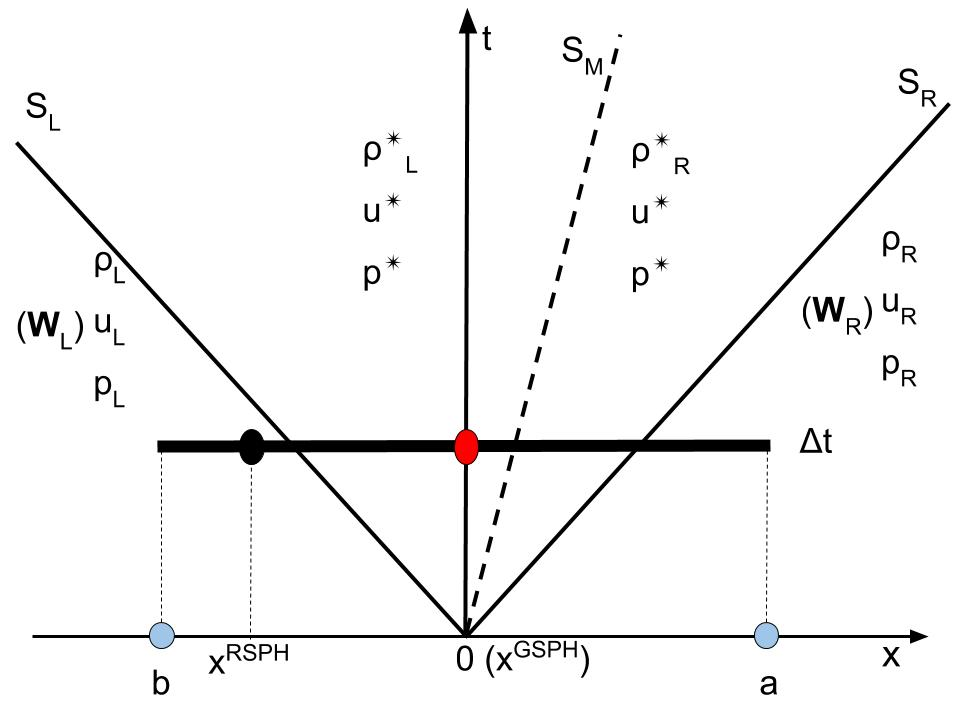
\includegraphics[width=0.5 \textwidth]{./Figures/RSPH-GSPH}
    \caption{Evaluating of the starred state for RSPH and GSPH implementations. $x$ is the local coordinate system for paired two particles, $a$ and $b$. The origin is at the middle of the paired two particles.
The local Riemann problem is defined by the constant states $(\rho, u, p)_a$ and $(\rho, u,p)_b$, namely $\textbf{W}_L = \textbf{W}_b$, $\textbf{W}_R = \textbf{W}_a$ with $\textbf{W} = (\rho, u,p)^T $, a vector representation of these three variables. The horizontal bold solid line at time $\Delta t$ indicates the interval on which to evaluate the solution of the Riemann problem. The dark ellipse is an example sample point of RSPH with the random number. The red ellipse indicates the stationary state, which is the starred state in GSPH. $S_L$, $S_M$ and $S_R$ are signal speeds which are linearized locally in HLLC Riemann solvers \citep{puri2014approximate}. Starred region is divided into two sub-regions by the middle contact wave. Only $\rho$ changes across the contact wave.}
    \label{fig:pick-up-state-GSPH-RSPH}
\end{figure}

The starred state $(u^{\ast},  p^{\ast})$ must now be projected back into the global coordinate system, to define  $(\textbf{v}^{\ast},  p^{\ast})$.

We mentioned that, instead of selecting a uniformly distributed random number $\epsilon$, we follow \citet{colella1982glimm} and adopt the Van Der Corput pseudo-random number sequence \citep{hammersley2013monte}.

\subsection{Non-iterative Riemann solvers} \label{sec:RP-solver}
Solving local Riemann problems exactly usually involves separating several cases of wave patterns and iteratively solving a small system of ordinary differential equations (for rarefaction waves) and a small set of nonlinear equations (the Rankine-Hugoniot equations). Instead of running this lengthy process one can employ approximate Riemann solvers, which provide an approximate solution quickly. There are many approximate Riemann solvers available \citep{rider1994review, luo2004computation, puri2014approximate}. For purposes here we adopt the HLLC solver, which decomposes the Riemann solution into 3 waves, including a (possible) contact discontinuity \cite{toro1994restoration}. More specifically, we adopt the HLLC formulation proposed by \citet{luo2004computation}.
 
We mention that, in the numerical tests in Section \ref{sec:numericaltests}, Both the HLLC solver and Roe solver are used for GSPH calculations.
To summarize, our RSPH algorithm proceeds as follows:
\begin{itemize}
\item For each pair of particles, establish a local coordinate system whose axis joins the particles,
and project the primitive variables onto this local coordinate system to define left and right states;
\item Solve this local Riemann problem approximately using a HLLC solver;
\item Sample the solution using the Van Der Corput sequence, defining a state  $p^{\ast}, u^{\ast}$;
\item Project $p^{\ast}, u^{\ast}$  back to the global coordinate system, to obtain $p^{\ast}$ and $\textbf{v}^{\ast}$;
\item Update the particle positions and physical quantities.
\end{itemize}

\section{Numerical tests} \label{sec:numericaltests}
We describe results from several numerical tests using SPH, RSPH and GSPH in this section.
A 1D shock tube test is investigated in different aspects to compare standard SPH, GSPH and RSPH revealing several features of RSPH. More shock tube simulations are also conducted to check the capacity of RSPH for different wave patterns. In addition, order of accuracy is investigated using the 1D shock tube problem. In the last subsection we describe a 3D free jet flow simulation. The effect of equivalent numerical dissipation is first demonstrated by SPH simulation with different artificial viscosity coefficients. Then the equivalent numerical dissipations introduced by GSPH and RSPH are compared demonstrating that RSPH introduces less dissipation than GSPH. In 3D fee jet flow simulation, local Riemann problems are constructed in a piece wise constant manner for both GSPH and RSPH.

Six 1D simulations described here are carried out:
\begin{itemize}% [1D Tests]
\item Test 1 consists of a left rarefaction, a right traveling contact and a right shock. Density increases at down wind of contact wave. 
\item Test 2 also consists of a left rarefaction, a right traveling contact and a right shock. Density decreases at down wind of contact wave. 
\item Test 3 includes double expansion waves. The initial density is different at right and left hand side. 
\item Test 4 is a double shocks test with different initial densities on the right side and left side.
\item Test 5 and Test 6 are two extreme cases. Test 5 is a cavity flow while test 6 is a strong blast flow.
\end{itemize}

\begin{table}[H]
\centering
      \caption{Overview of 1D shock tube tests}		
	  \begin{tabular}{lrrrrrrrrrr}
	    \hline
	          & $\rho_L$ & $p_L$ &$v_L$ & $\rho_R$ & $p_R$ &$v_R$ & $m$ & $[x_L, x_R]$ & $t_f$\\
	    \hline
	    Test 1 & $1.0$ & $1.0$ &$0$ & $0.25$ & $0.1795$ &$0$ & $0.003$  & $[-0.4, 0.4]$ & $0.17$\\
	    	Test 2 & $1.0$ & $1.0$ &$0$ & $0.5$ & $0.2$ &$0$ & $0.003$  & $[-0.4, 0.4]$ & $0.2$\\
	    	Test 3 & $2.0$ & $1.95$ &$-1.0$ & $1.0$ & $1.95$ &$1.0$  & $0.006$  & $[-0.4, 0.4]$ & $0.13$\\
	    Test 4 & $1.0$ & $2.4$ &$8.0$ & $0.5$ & $0.4$ &$-0.25$ & $0.003$  & $[-0.4, 0.4]$ & $0.05$\\
	    	Test 5 & $1.0$ & $0.4$ &$-2.0$ & $1.0$ & $0.4$ &$2.0$ & $0.003$  & $[-0.4, 0.4]$ & $0.18$\\
	    	Test 6 & $1.0$ & $1000$ &$0$ & $1.0$ & $0.01$ &$0$ & $0.003$  & $[-0.5, 0.5]$  & $0.01$\\
	    \hline
	  \end{tabular}
	  \label{tab:1D-shock-input_parameters}
\end{table}
Input parameters for 1D tests can be found in Table \ref{tab:1D-shock-input_parameters}, where, subscript $L$ refers left side and $R$ for right side. $m$ is particle mass, initial interval between adjacent particles are adjusted to guarantee equal particle mass. $t_f$ is the time to terminate simulation and plotting the results. The $x$ axis in all plots is normalized by time, that is $x/t_f$, in plots for shock tube tests results.

In first four tests, density on right and left sides are different. Considering that all particles have the same particle mass, assigning smoothing length according to $h \propto \frac{m}{\rho}$ leads to discontinuity of smoothing length at the middle. Such discontinuity of smoothing length is the source of numerical oscillations, which usually decay fast and are not observed when there is sufficient dissipation. 
Such numerical oscillation becomes obvious when dissipation is less. For example, when SPH taking $\alpha=0.2$ (see Fig. \ref{fig:RCM-Sod-SPH-alf} and Fig. \ref{fig:RCM-Sod-SPH-alf-zoom}). That is to say, how much the numerical oscillation is suppressed can indicate the amount of numerical dissipation introduced in each SPH scheme providing we are solving inviscid fluids (no physical dissipation). Refer Appendix B for more information regarding the numerical oscillation due to nonuniform smoothing length.
Another indicator of numerical dissipation is how much the shock is smeared. Both indicators reflect consistent information regarding numerical dissipation throughout our tests, see, for example, plot c) in Fig. \ref{fig:RCM-Sod-SPH-alf-zoom} or plot g) in Fig. \ref{fig:RCM-GSPH-Sod}. 
We take these two as indicators of numerical dissipation in many discussions regarding 1D tests.
As for 3D jet flow, we take the distance between jet head and inject vent at given physical time as the indicator of overall equivalent numerical dissipation. As shown in Fig. \ref{fig:free-jet-SPH-comparison}, the distance between jet head and inject vent decrease when artificial viscosity coefficients increase. This confirms that such distance do reflect overall equivalent dissipation.

\subsection{Comparison of RSPH with standard SPH and GSPH}

\begin{figure}[H]
    \centering
    \begin{minipage}{.45\textwidth}
        \centering a)
        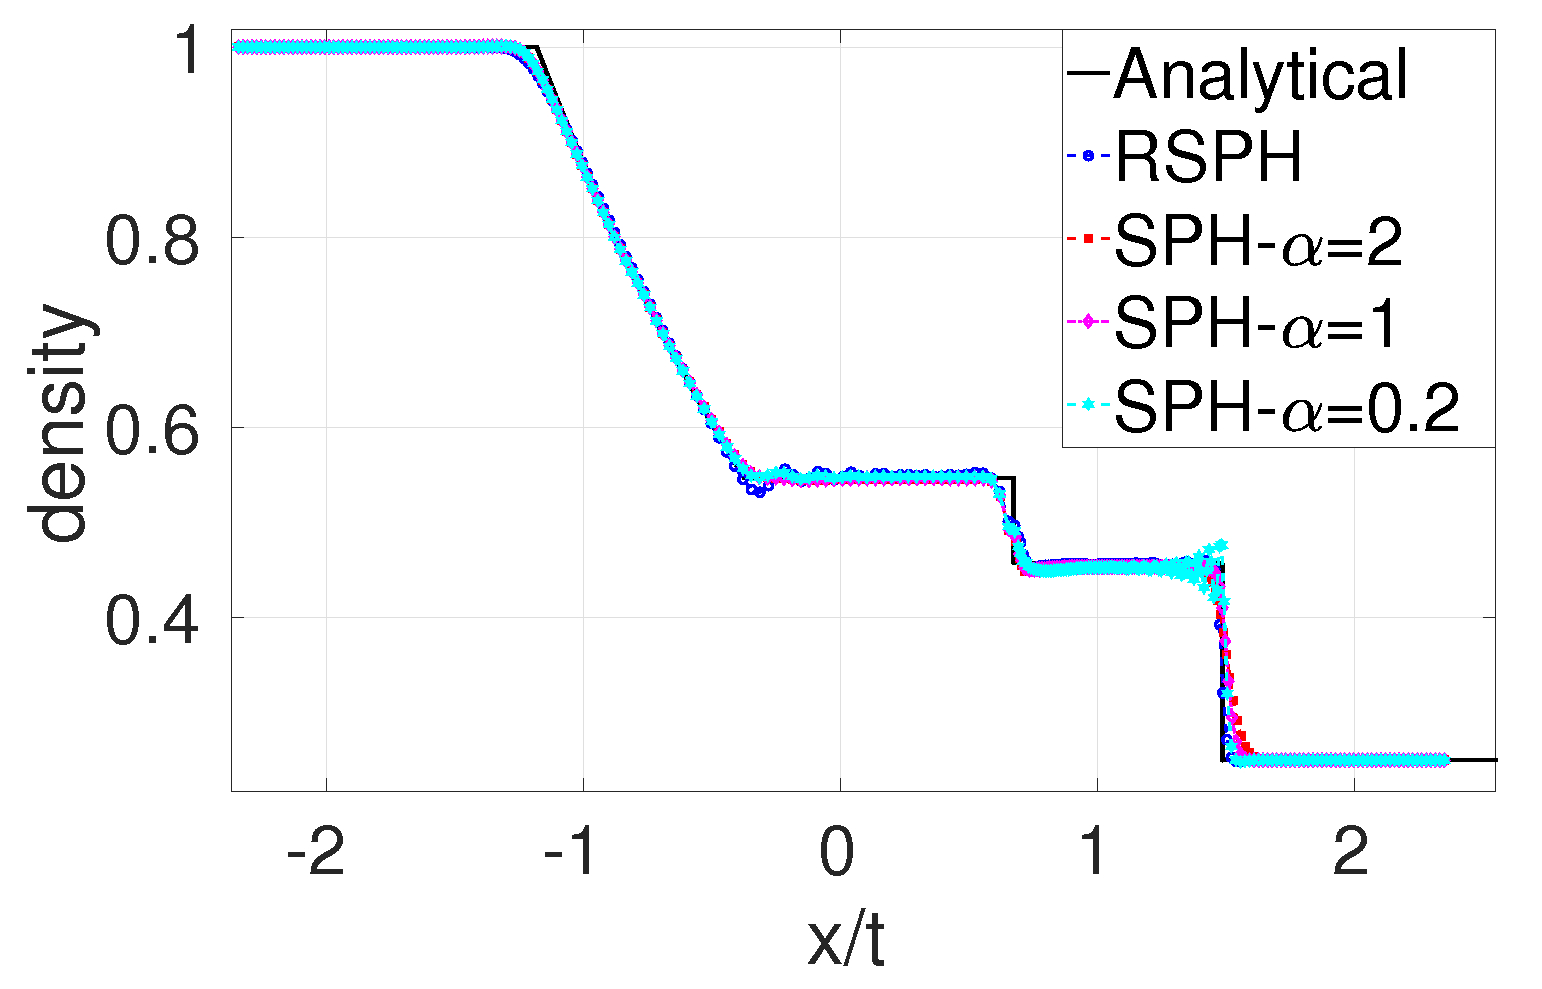
\includegraphics[width=0.99 \textwidth,height=0.7\textwidth]{./Figures/RCM-Sod-SPH-alf-rho}
    \end{minipage}%
    \begin{minipage}{.545 \textwidth}
        \centering b)
        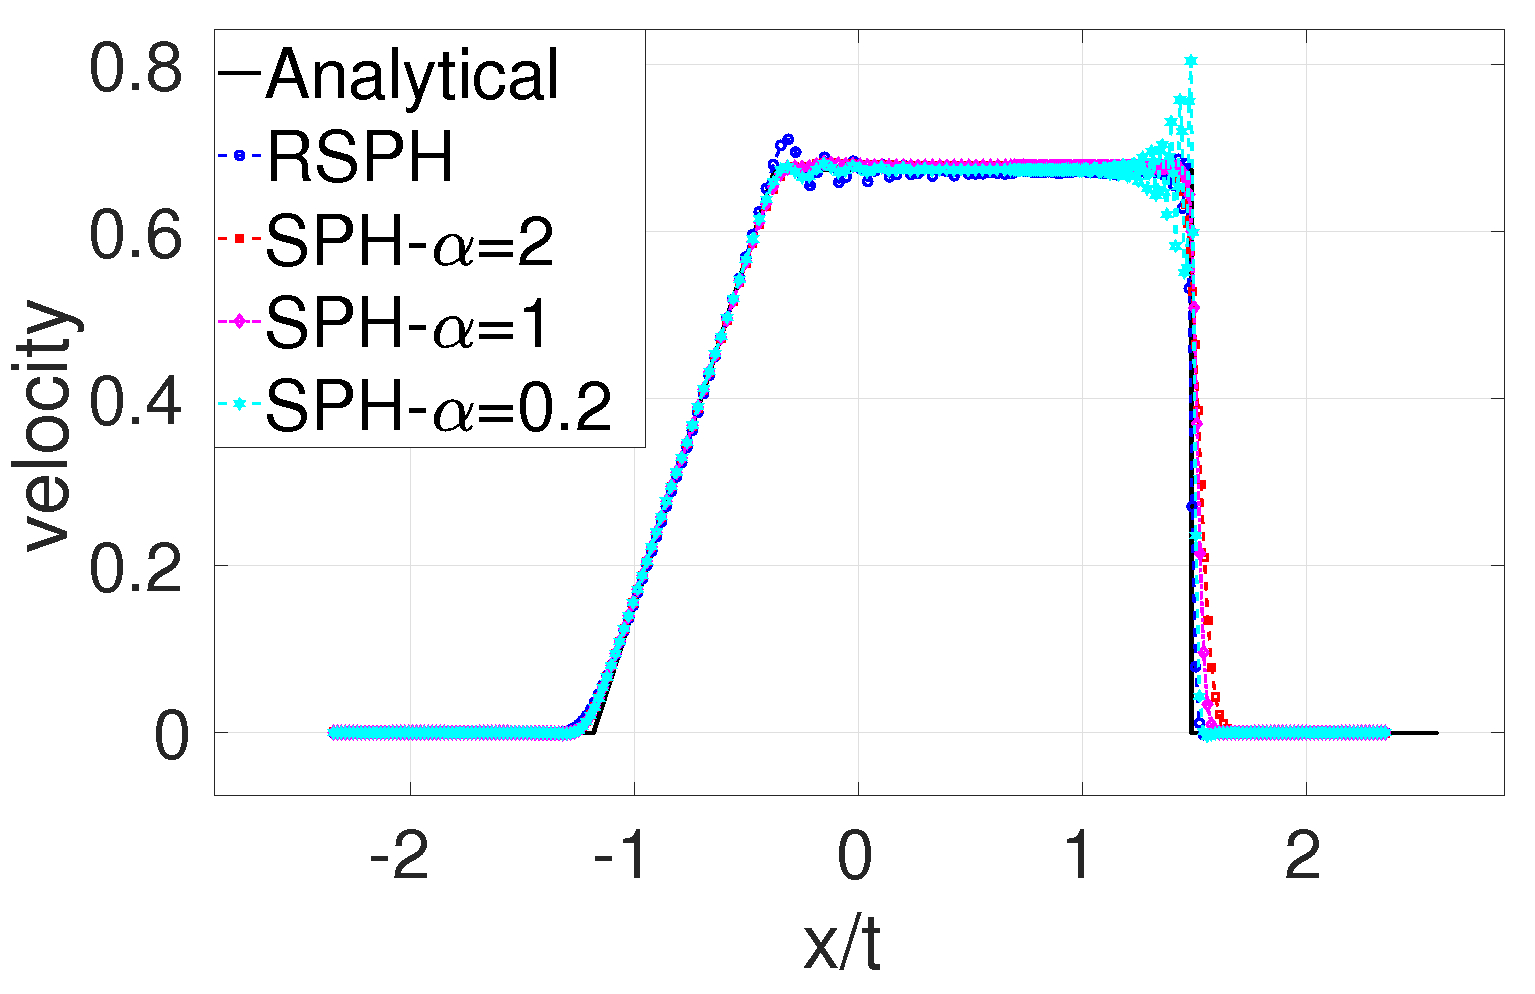
\includegraphics[width=0.99 \textwidth,height=0.5780 \textwidth]{./Figures/RCM-Sod-SPH-alf-v}
    \end{minipage}% 
    \\
    \begin{minipage}{.45 \textwidth}
        \centering c)
        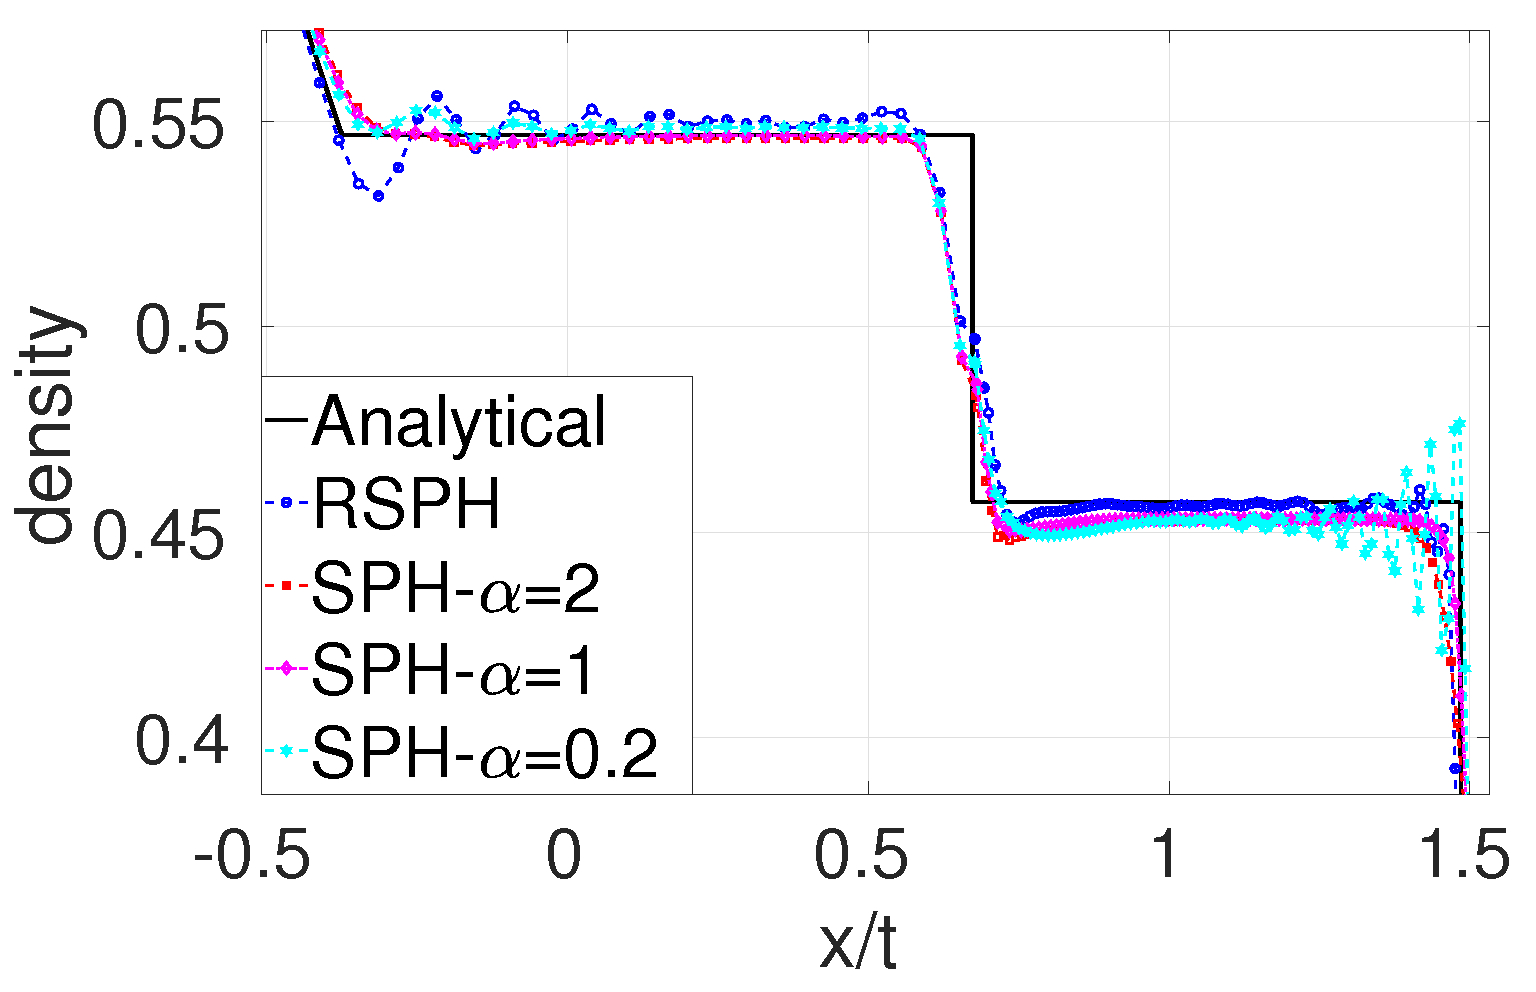
\includegraphics[width=0.99 \textwidth, height=0.7\textwidth]{./Figures/RCM-Sod-SPH-alf-rho-zoom}
    \end{minipage}% 
    \begin{minipage}{.545\textwidth}
    \centering d)
        \begin{flushleft}
        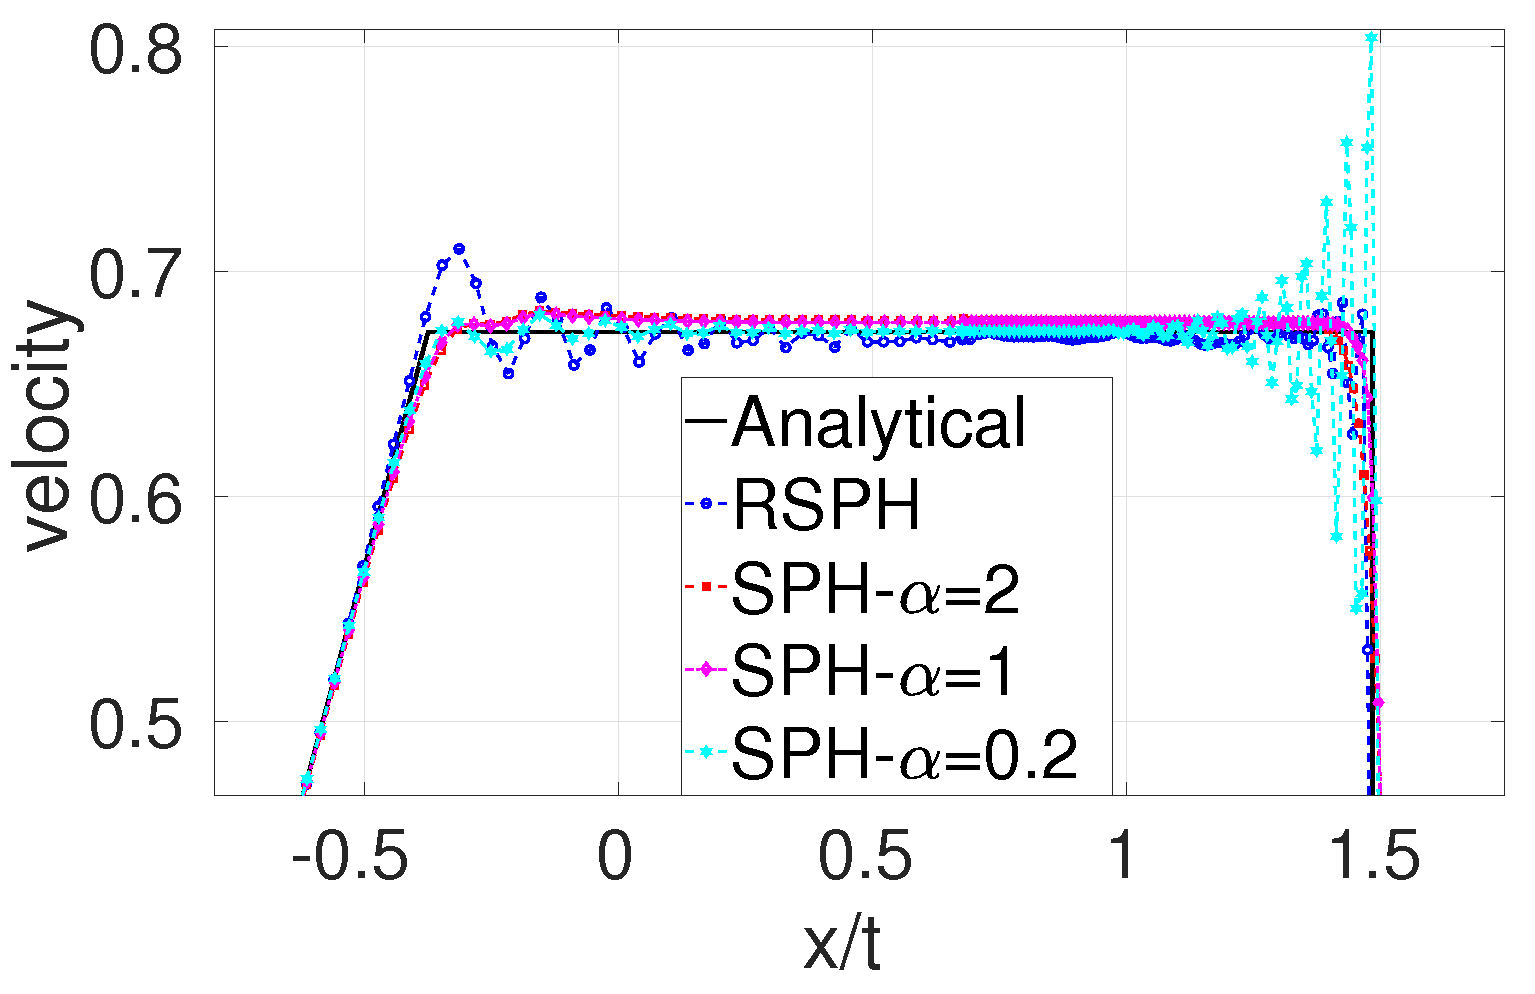
\includegraphics[width= 0.8174 \textwidth, height=0.5780 \textwidth]{./Figures/RCM-Sod-SPH-alf-v-zoom}    
        \end{flushleft}
    \end{minipage}%          
    \caption{a) and b) are plots for density and velocity in Test 1 by RSPH and SPH with different artificial viscosity coefficients. $\alpha,\beta$ satisfies: $\beta=2\alpha$.  c), d) are corresponding zoomed views. SPH simulations with different artificial viscosity coefficients show that numerical oscillation is obvious, especially around shock, if there is insufficient dissipation ($\alpha=0.2$). The dissipation introduced by RSPH, is shown to be more adaptive, introducing more damping at the shock (comparable to $\alpha=1.0$) and less damping in the area away from the shock (less than $\alpha=0.2$, as indicated by the magnitude of numerical oscillation).}
    \label{fig:RCM-Sod-SPH-alf}
\end{figure}

\begin{figure}[H]
    \centering
    \begin{minipage}{.45\textwidth}
        \centering a)
        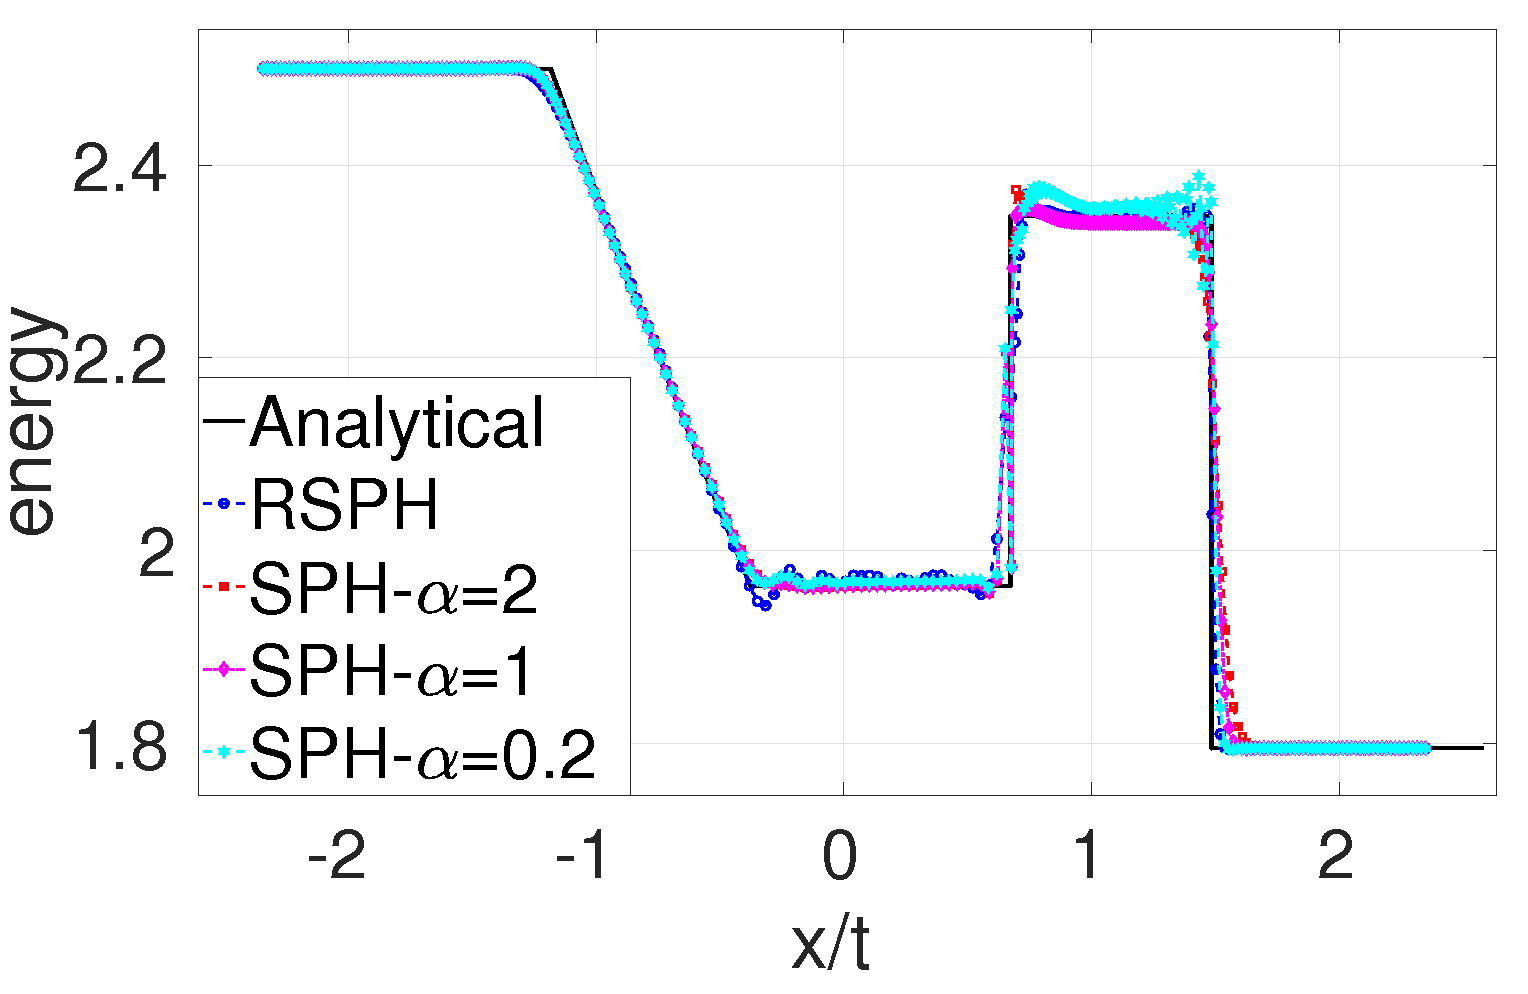
\includegraphics[width=0.99 \textwidth,height=0.7\textwidth]{./Figures/RCM-Sod-SPH-alf-e}
    \end{minipage}%
    \begin{minipage}{.545 \textwidth}
        \centering b)
        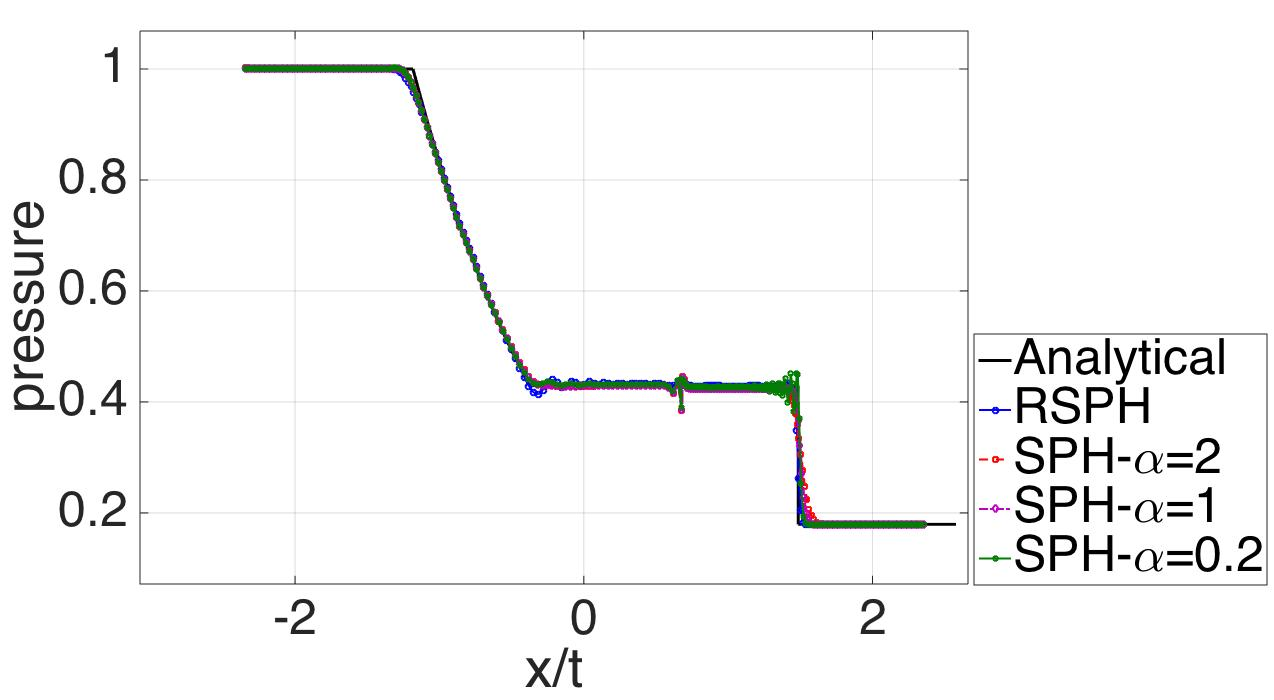
\includegraphics[width=0.99 \textwidth,height=0.5780 \textwidth]{./Figures/RCM-Sod-SPH-alf-p}
    \end{minipage}% 
    \\
    \begin{minipage}{.45 \textwidth}
        \centering c)
        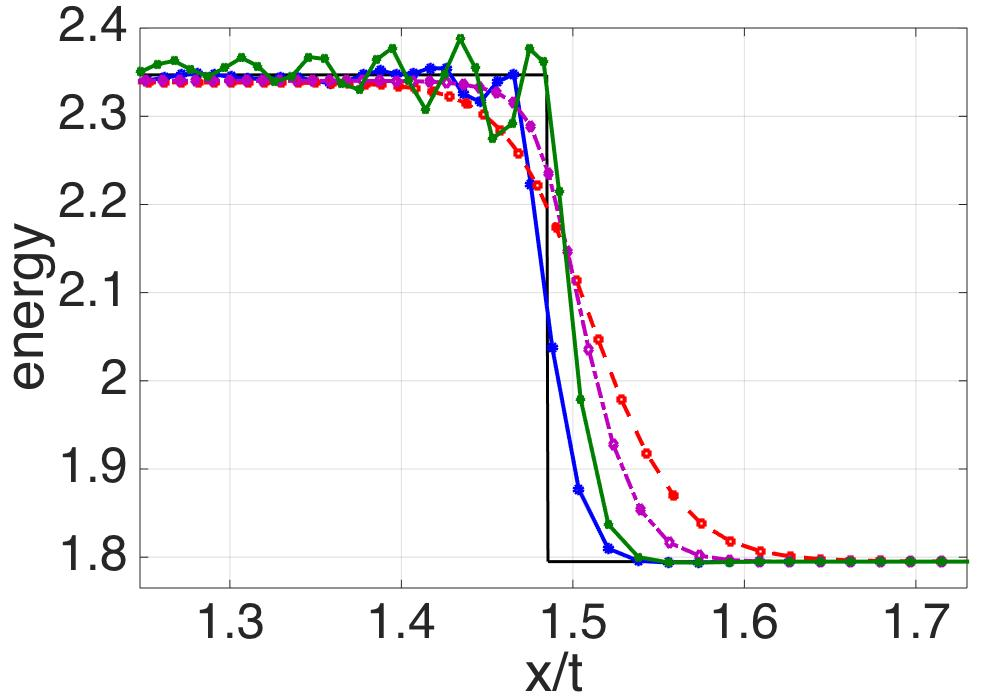
\includegraphics[width=0.99 \textwidth, height=0.7\textwidth]{./Figures/RCM-Sod-SPH-alf-e-zoom}
    \end{minipage}% 
    \begin{minipage}{.545\textwidth}
    \centering d)
        \begin{flushleft}
        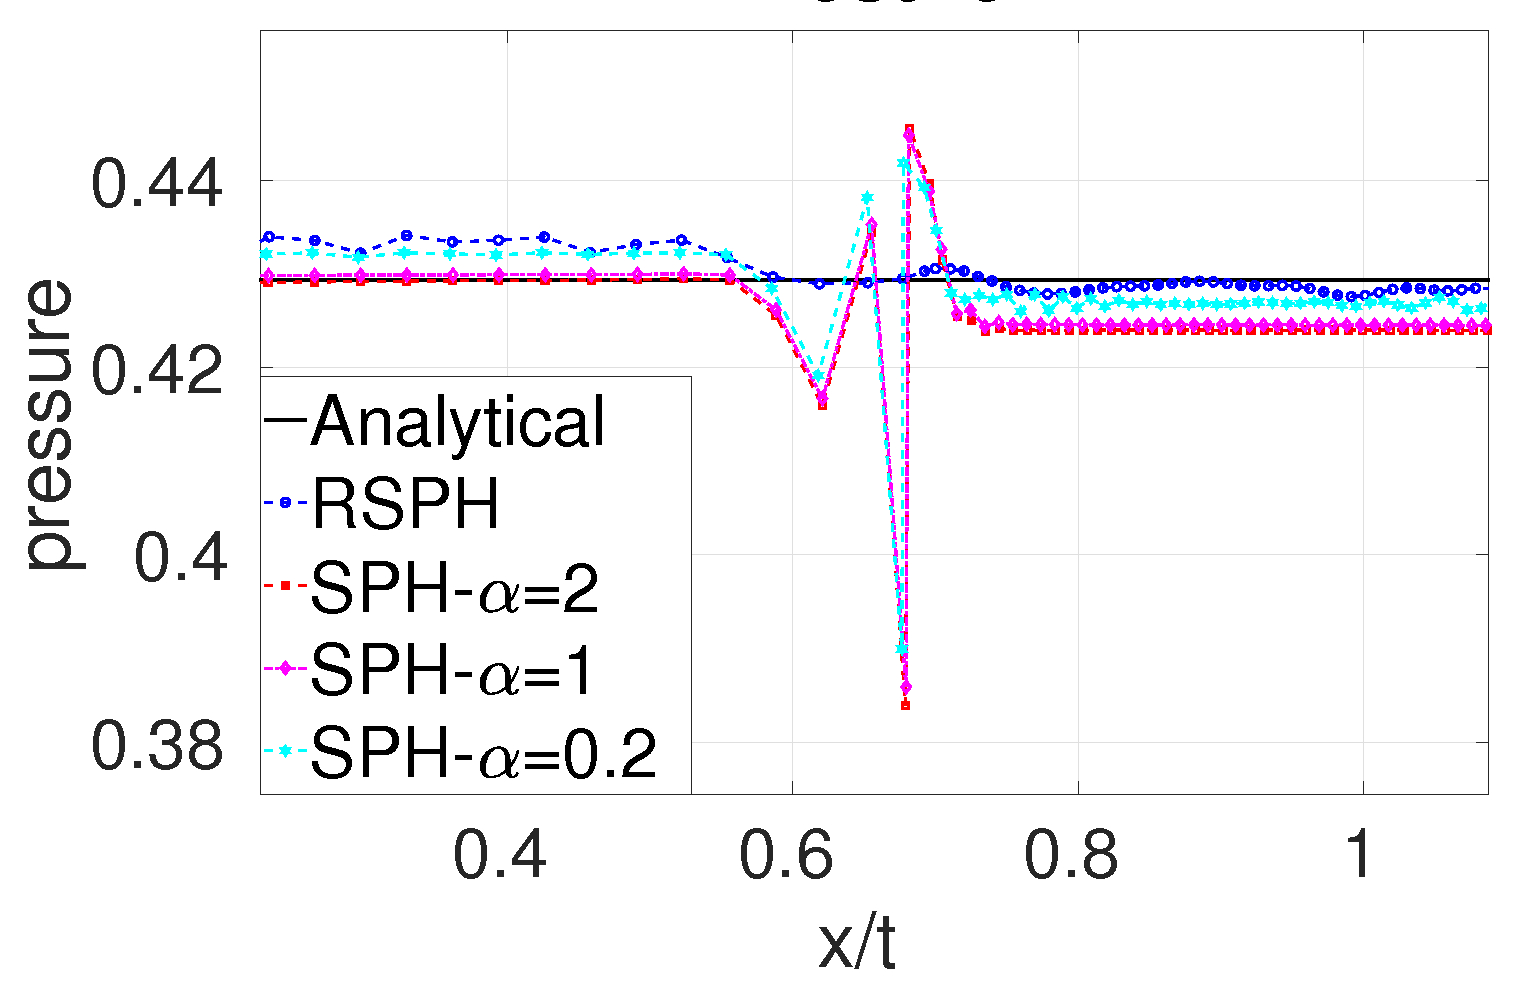
\includegraphics[width= 0.8174 \textwidth, height=0.5780 \textwidth]{./Figures/RCM-Sod-SPH-alf-p-zoom}    
        \end{flushleft}
    \end{minipage}%    
    \caption{
    a), b) are plots of internal energy and pressure in Test 1 by RSPH and SPH with different artificial viscosity coefficients.  c), d) are corresponding zoomed views. For $\alpha=1$ and $\alpha=2$, as shown in c), numerical oscillations are completely suppressed. However there is also more smearing around the shock. $\alpha=0.2$ provides insufficient viscosity to suppress oscillations while the smearing around the shock is also less. Impressively, RSPH is showing to introduce adaptive dissipation, more dissipative at the shock (comparable or better than $\alpha=1.0$) and less dissipative away from the shock (less than $\alpha=0.2$). d) shows pressure around the contact discontinuity. It is evident that RSPH gets rid of the pressure ``wiggle" around the contact discontinuity.}
    \label{fig:RCM-Sod-SPH-alf-zoom}
\end{figure}

Test 1 is simulated using standard SPH with different artificial viscosity coefficients, GSPH and RSPH. Results are checked from different aspects.  
The comparison between RSPH and SPH with different artificial viscosity coefficients is shown in Fig. \ref{fig:RCM-Sod-SPH-alf} and \ref{fig:RCM-Sod-SPH-alf-zoom}. In all SPH simulations, the artificial viscosity coefficient $\beta$ is set to be twice of $\alpha$. For example, for the test ``$SPH-\alpha=2$", $\beta=4$.

Several interesting observations are made based on the comparison between SPH and RSPH.
First of all, dissipation (introduced by artificial viscosity in these tests) decays the numerical fluctuations. Numerical fluctuations are suppressed completely when large dissipation is introduced, for example, by using sufficiently large artificial viscosity coefficients ($\alpha=1,2$).
Secondly, the equivalent artificial viscosity introduced by RSPH varies more adaptively.
As shown in Fig. \ref{fig:RCM-Sod-SPH-alf} and \ref{fig:RCM-Sod-SPH-alf-zoom}, RSPH assigns smaller artificial viscosity (equivalent $\alpha$ much less then 0.2) at the area far away from shock and sufficiently large artificial viscosity coefficients (equivalent $\alpha$ is about 1.0) around the shock. Namely, RSPH adaptively assigns larger equivalent artificial viscosity coefficient around the shock and take smaller equivalent artificial viscosity far away from shock. This feature is very desirable not only because it could eliminate parameterization and hence user intervention associated with artificial viscosity coefficients but also because it avoids introducing excess artificial viscosity.
Thirdly, RSPH introduces less smearing of the shock discontinuity compared with SPH using most commonly adopted artificial viscosity coefficients ($\alpha=1.0$, $\beta=2.0$). Recall that RCM is able to resolve discontinuities as true discontinuity. RSPH, even though it still smears the discontinuity in some degree, introduces much less smearing (see Fig. \ref{fig:RCM-Sod-SPH-alf-zoom}).
The last but not the least, the pressure ``wiggle" around contact discontinuity is completely eliminated by RSPH as seen in Fig. \ref{fig:RCM-Sod-SPH-alf-zoom}. \citet{inutsuka2002reformulation} show that GSPH can almost get rid of pressure wiggle around contact discontinuity while standard SPH has much more obvious pressure wiggle. 
%They believe that the pressure wiggle is due to the inconsistency of equation of momentum in the standard SPH discretization. However, there are different opinions with respect to the sources of pressure wiggle. It has been shown that thermal conduction is essential to mitigate the spurious pressure ``wiggle" at contact discontinuity in SPH \citep{monaghan1997sph, sigalotti2006shock, price2008modelling, price2012smoothed}.
%As for GSPH, it is reported that an implicit thermal conduction is introduced by Godunov's scheme and helps suppress the anomaly \citep{puri2014approximate}.
 Even though, the ``wiggle" still visible in pressure distribution and velocity distribution of GSPH simulation results (for example, see figures in \citep{puri2014comparison}) and RSPH simulation results of other tests (see section \ref{sec:comprehensive-1d-tests}). Pressure wiggle in test 1, however, is completely eliminated by both GSPH and RSPH.

\begin{figure}[H]
    \centering
    \begin{minipage}{.45\textwidth}
        \centering a)
        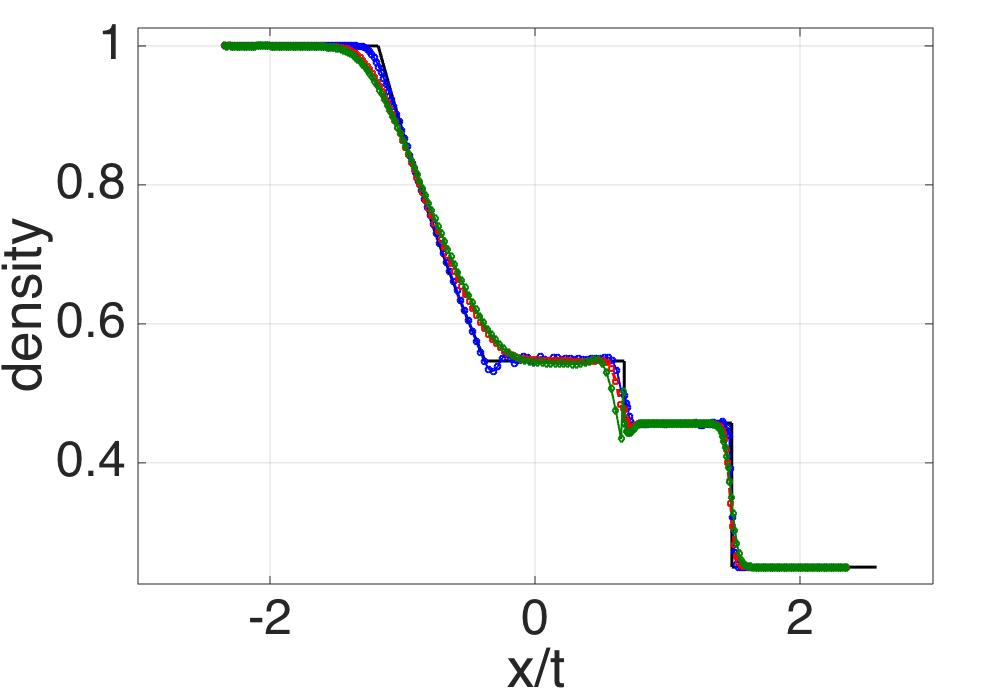
\includegraphics[width=0.99 \textwidth,height=0.6\textwidth]{./Figures/RCM-Sod-GSPH-compare-rho}
    \end{minipage}%
    \begin{minipage}{.545\textwidth}
    \centering b)
        \begin{flushleft}
        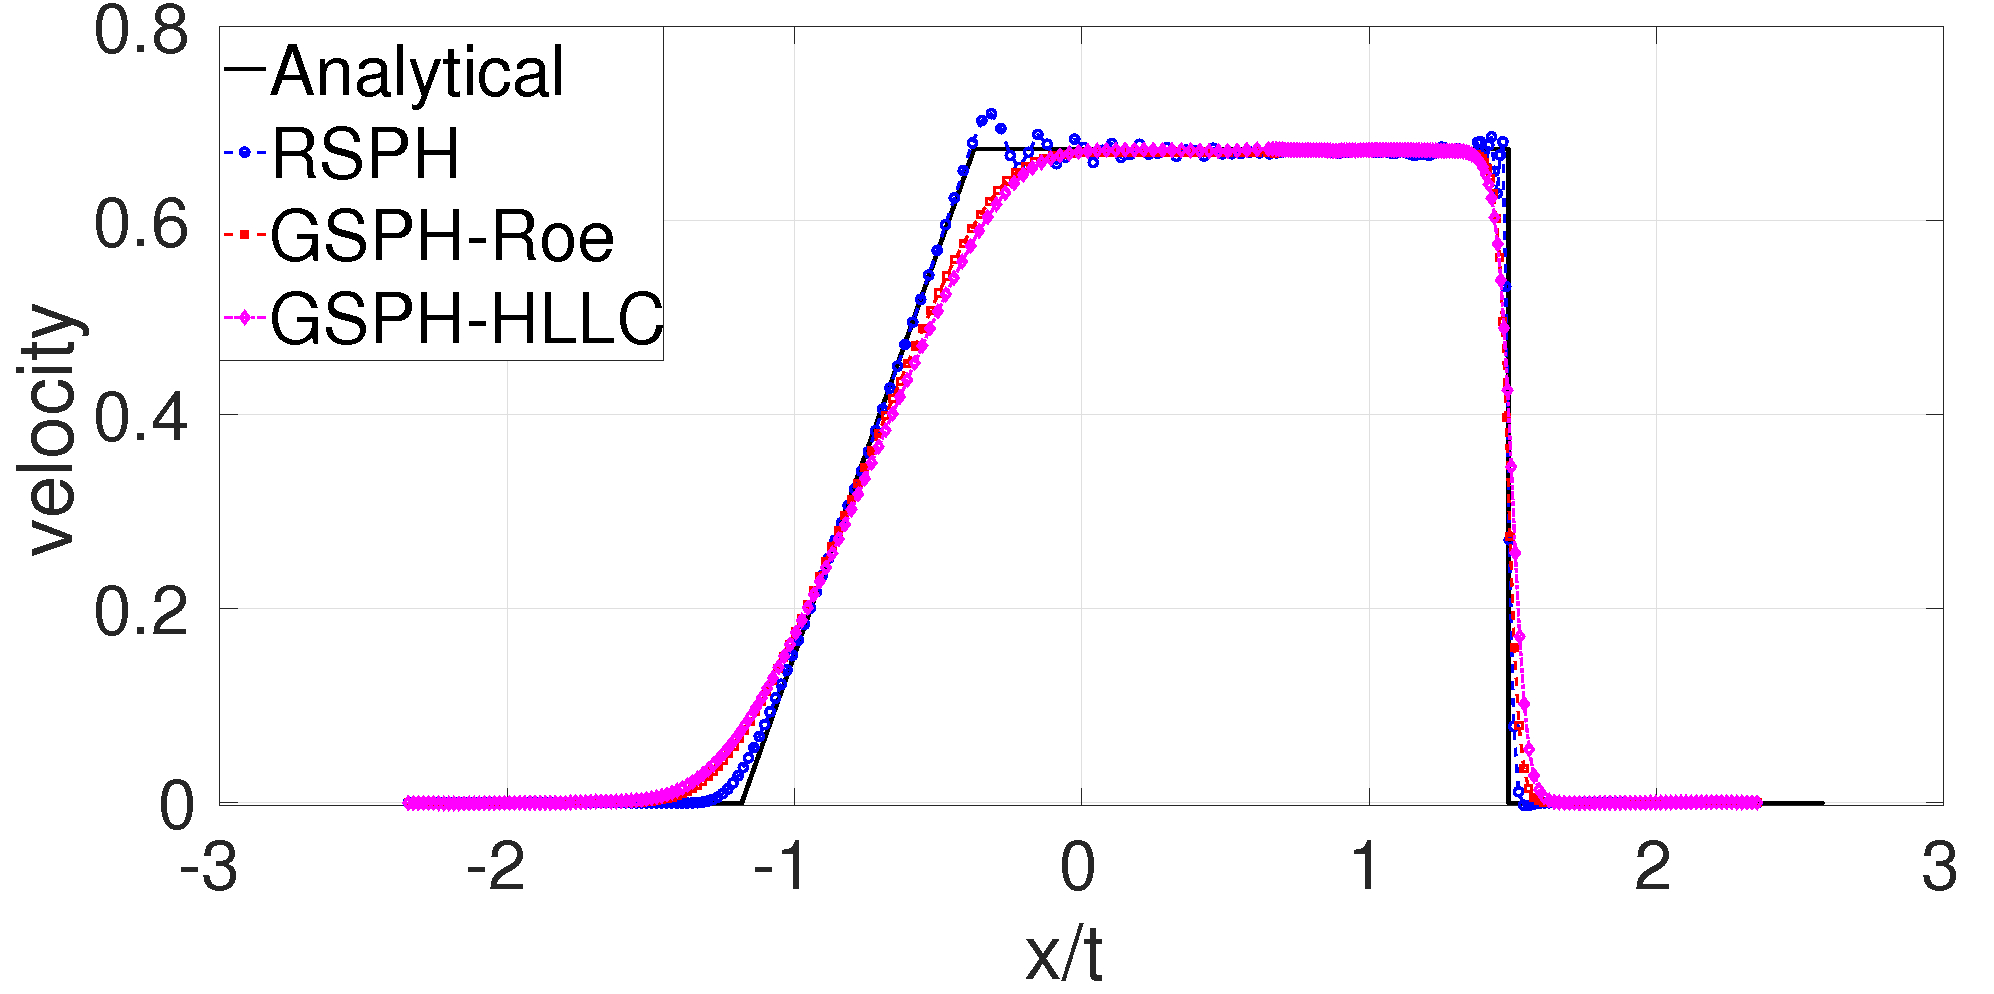
\includegraphics[width= 0.8174 \textwidth, height=0.4954 \textwidth]{./Figures/RCM-Sod-GSPH-compare-v}    
        \end{flushleft}
    \end{minipage}% 
    \\
    \begin{minipage}{.45\textwidth}
        \centering c)
        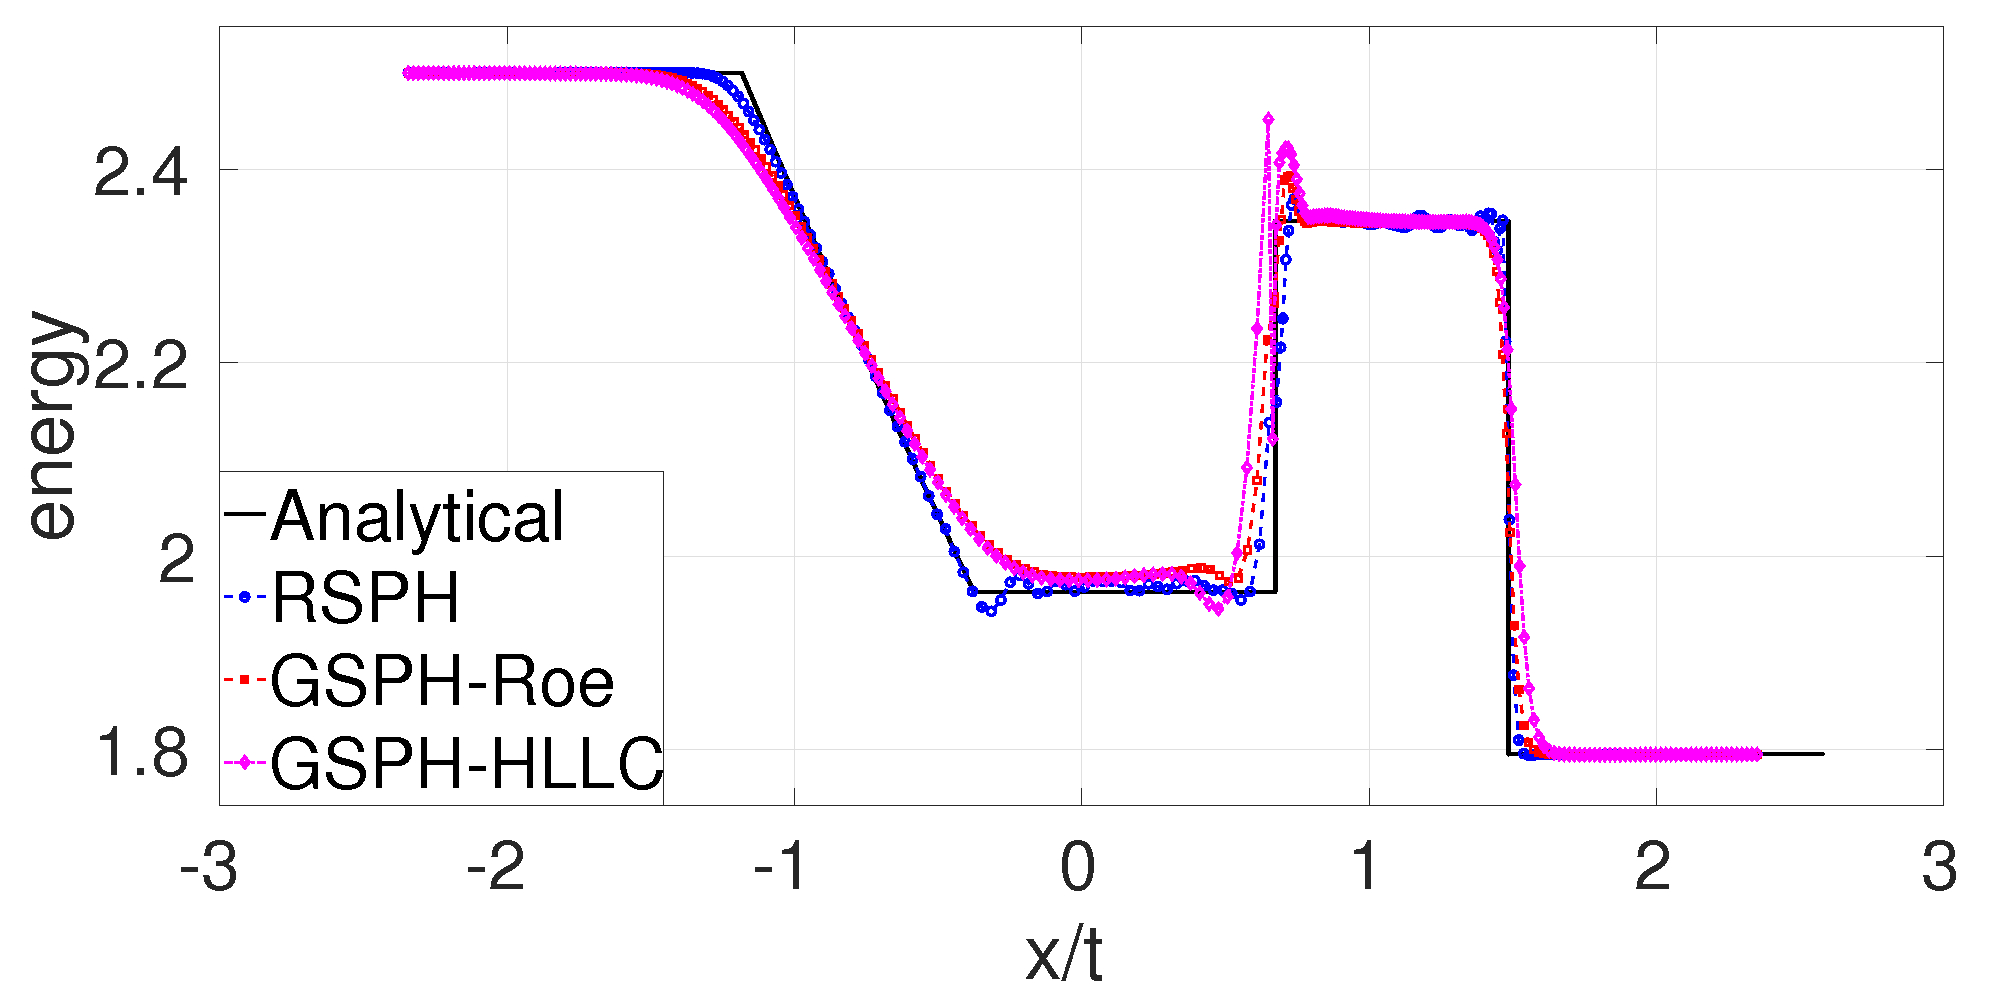
\includegraphics[width=0.99 \textwidth,height=0.6\textwidth]{./Figures/RCM-Sod-GSPH-compare-e}
    \end{minipage}%
    \begin{minipage}{.545 \textwidth}
        \centering d)
        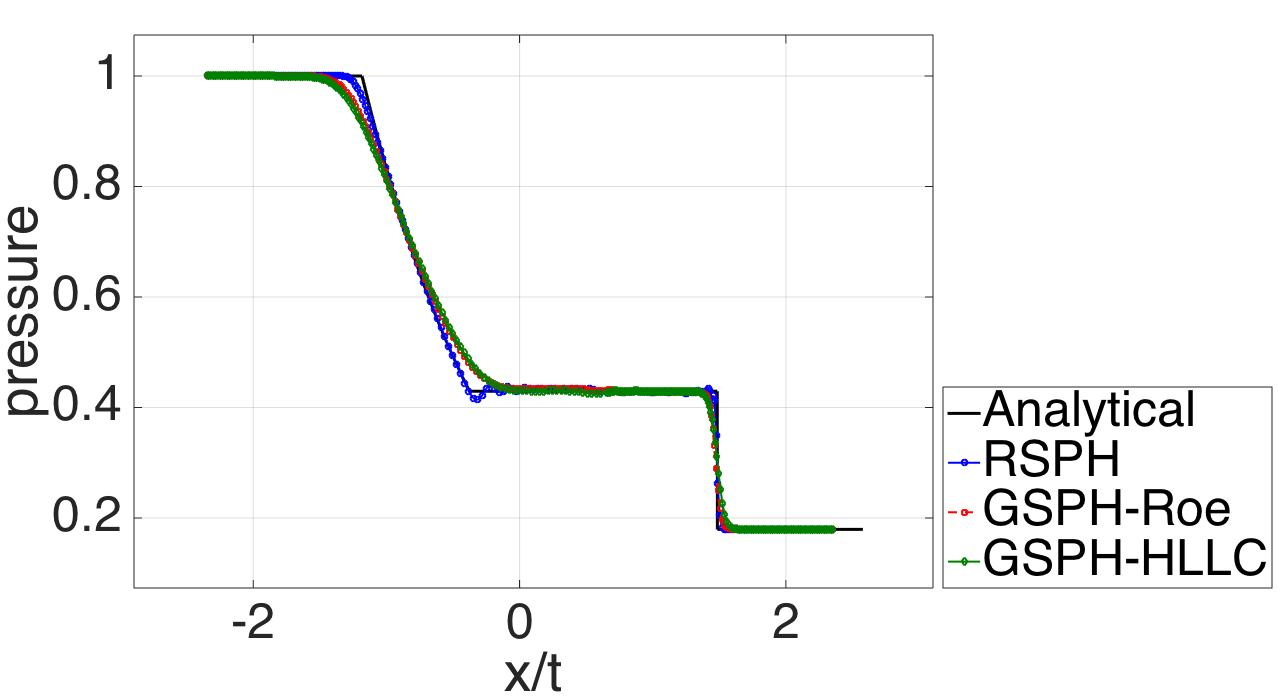
\includegraphics[width=0.99 \textwidth,height=0.4954\textwidth]{./Figures/RCM-Sod-GSPH-compare-p}
    \end{minipage}% 
    \\
    \begin{minipage}{.45\textwidth}
        \centering e)
        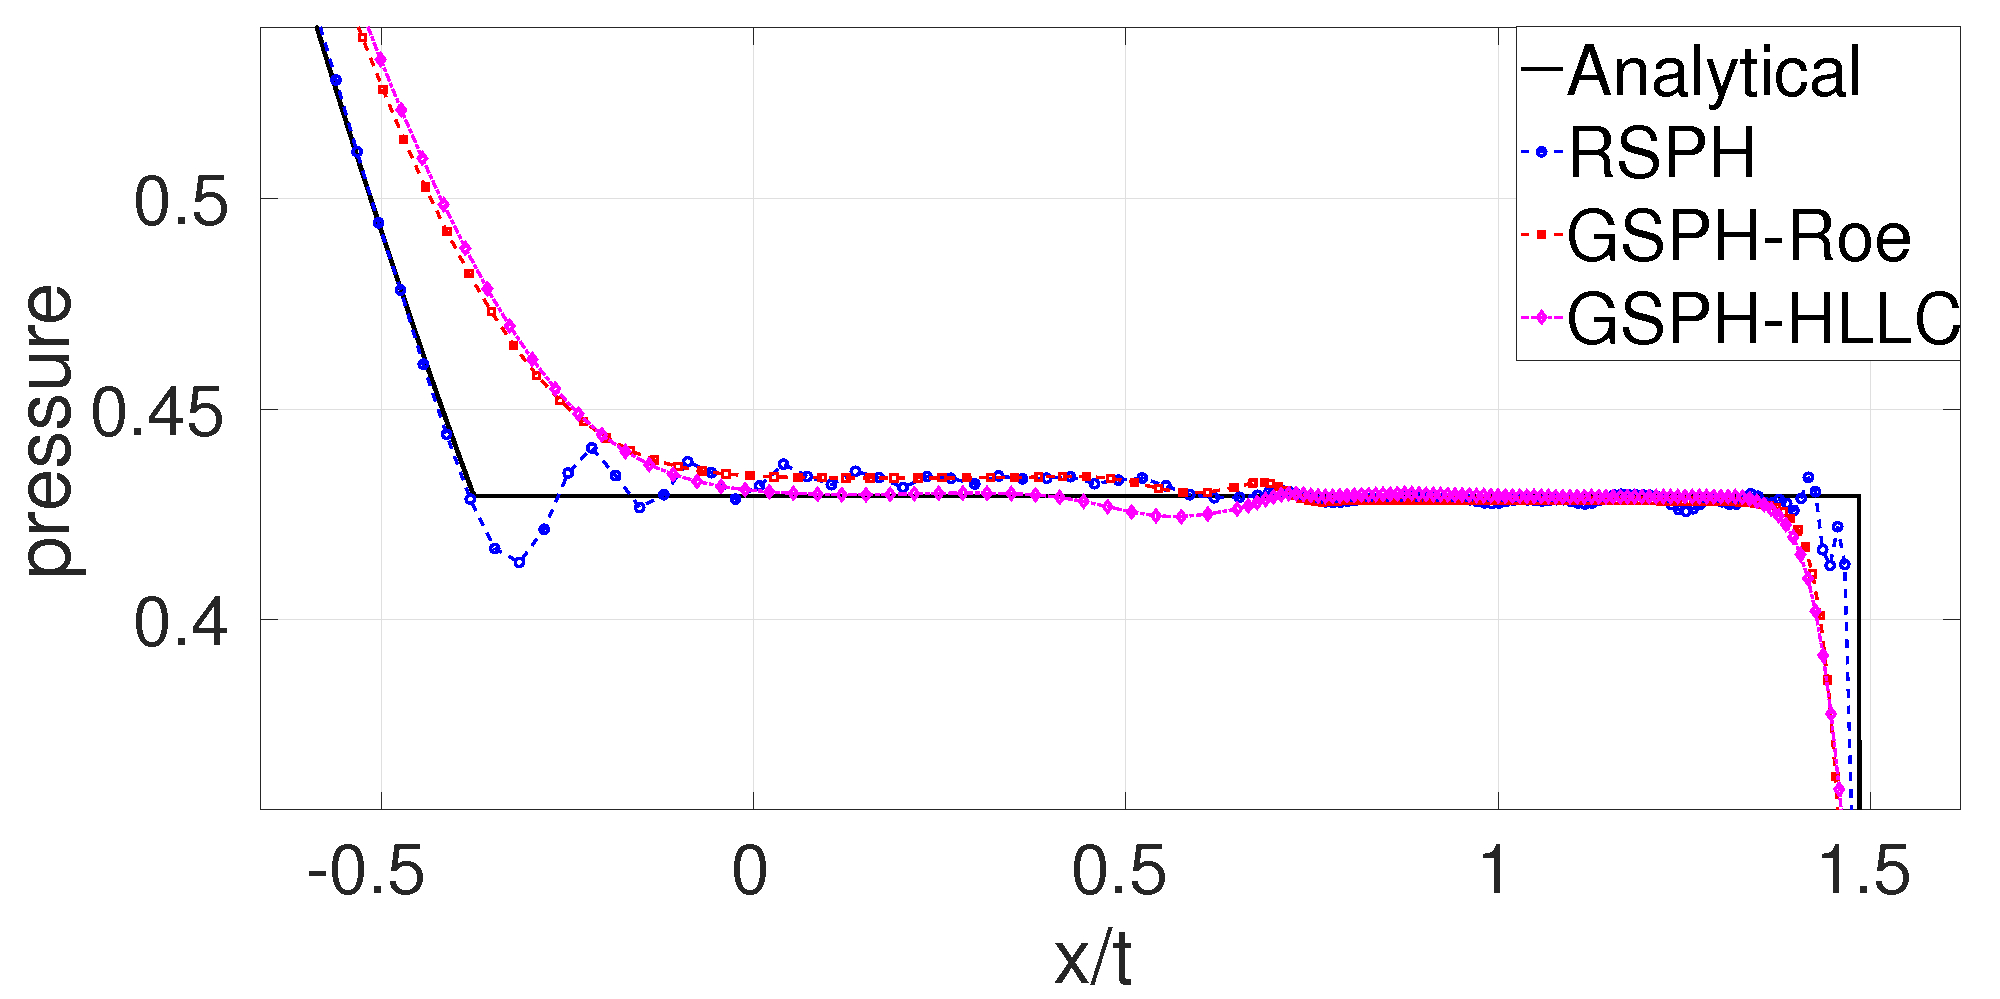
\includegraphics[width= 0.99 \textwidth, height=0.625 \textwidth]{./Figures/RCM-Sod-GSPH-compare-p-zoom}    
    \end{minipage}%
    \begin{minipage}{.545\textwidth}
        \centering f)
        \begin{flushleft}
        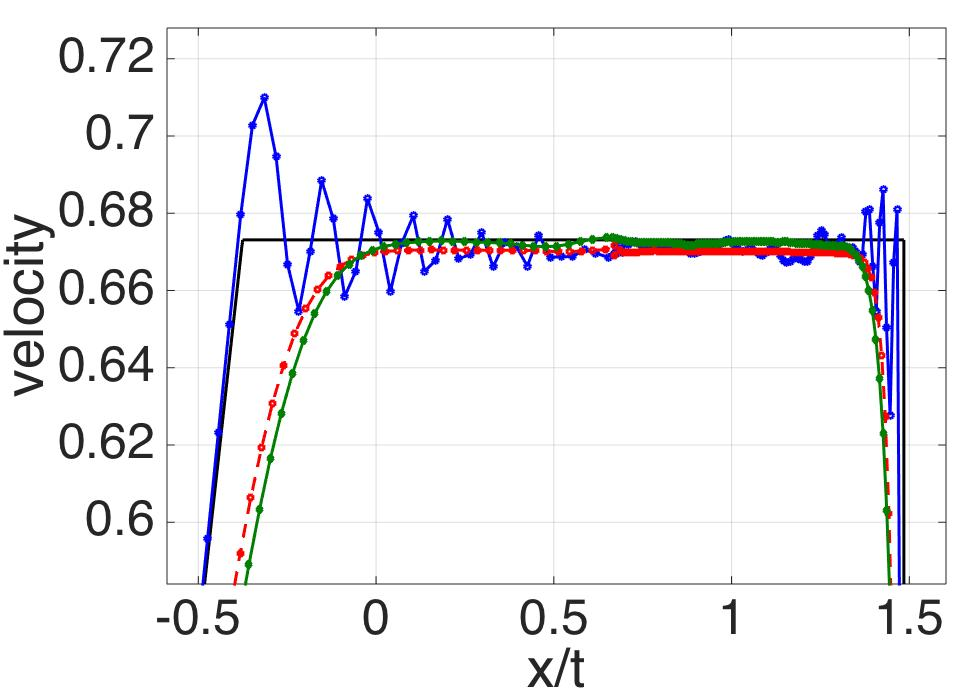
\includegraphics[width= 0.8174 \textwidth, height=0.4954 \textwidth]{./Figures/RCM-Sod-GSPH-compare-v-zoom}    
        \end{flushleft}
    \end{minipage}%  
%    \begin{minipage}{.45\textwidth}
%        \centering e)
%        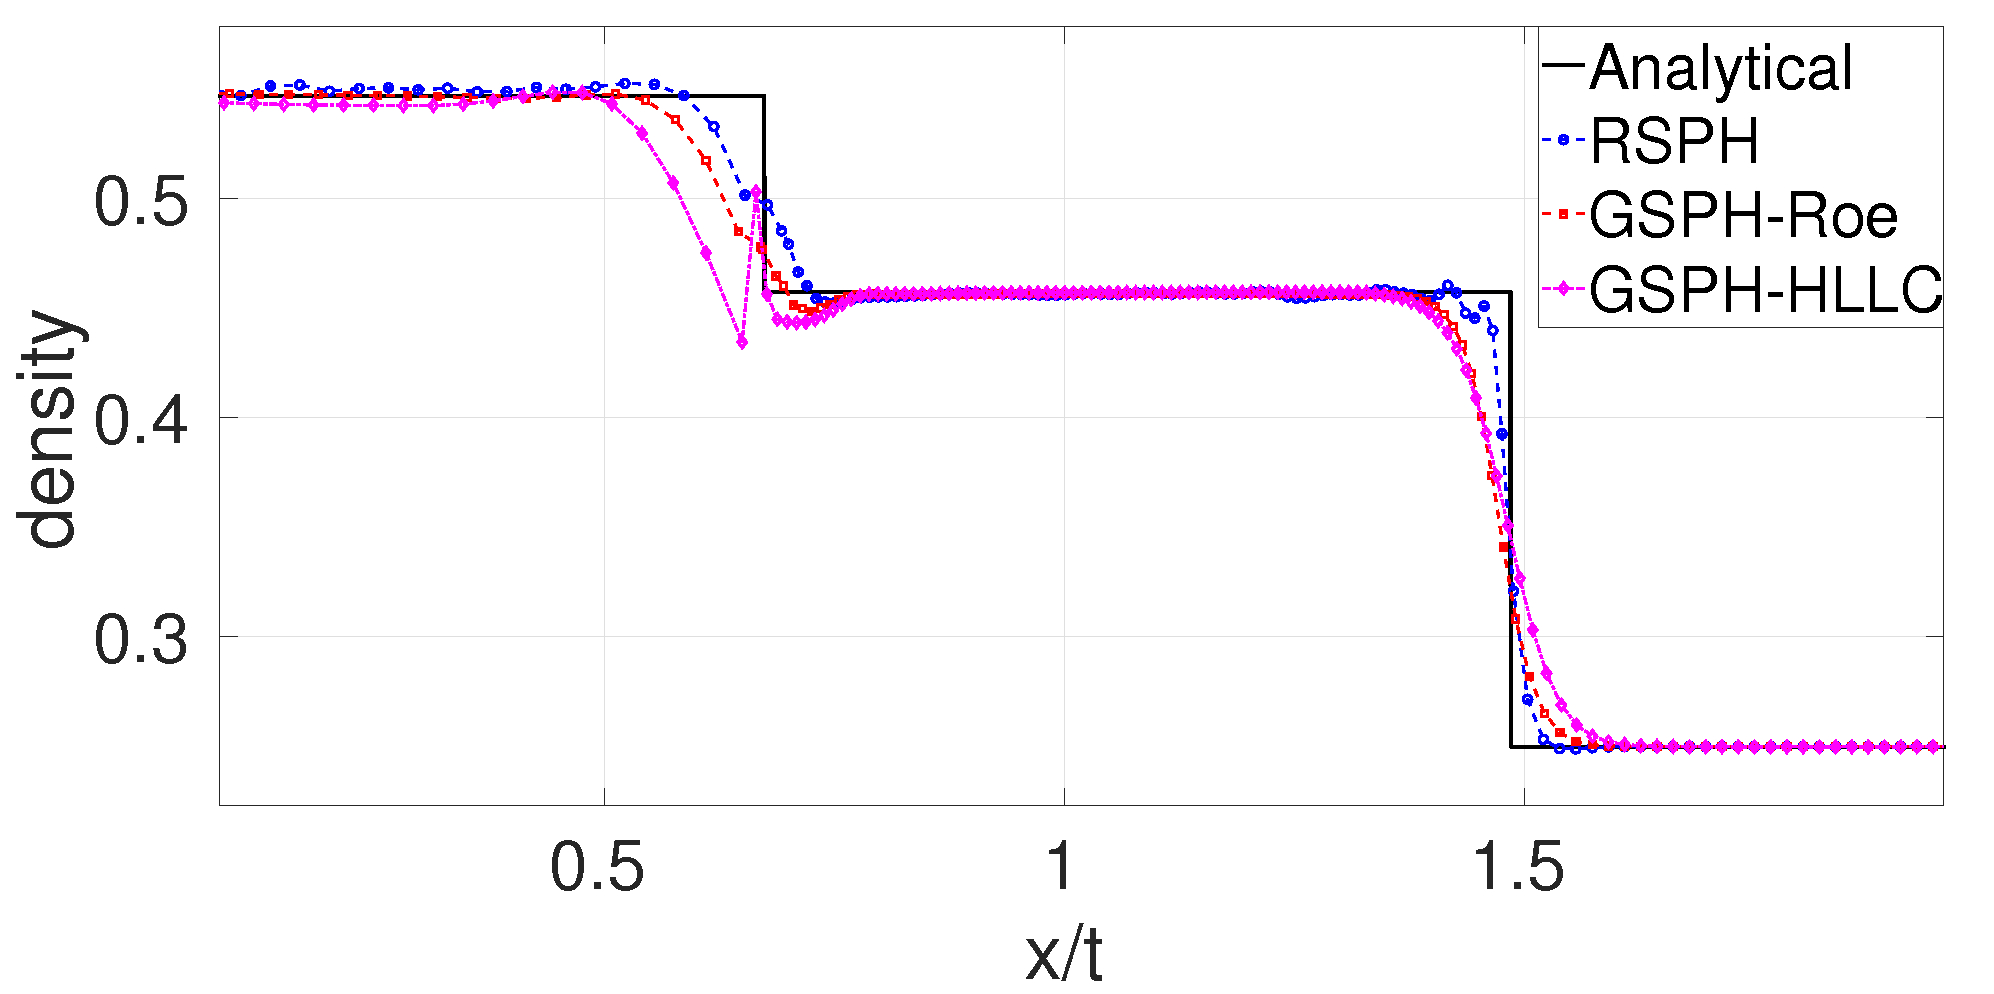
\includegraphics[width=0.99 \textwidth,height=0.6\textwidth]{./Figures/RCM-Sod-GSPH-compare-rho-zoom}
%    \end{minipage}%
%    \begin{minipage}{.545\textwidth}
%    \centering f)
%        \begin{flushleft}
%        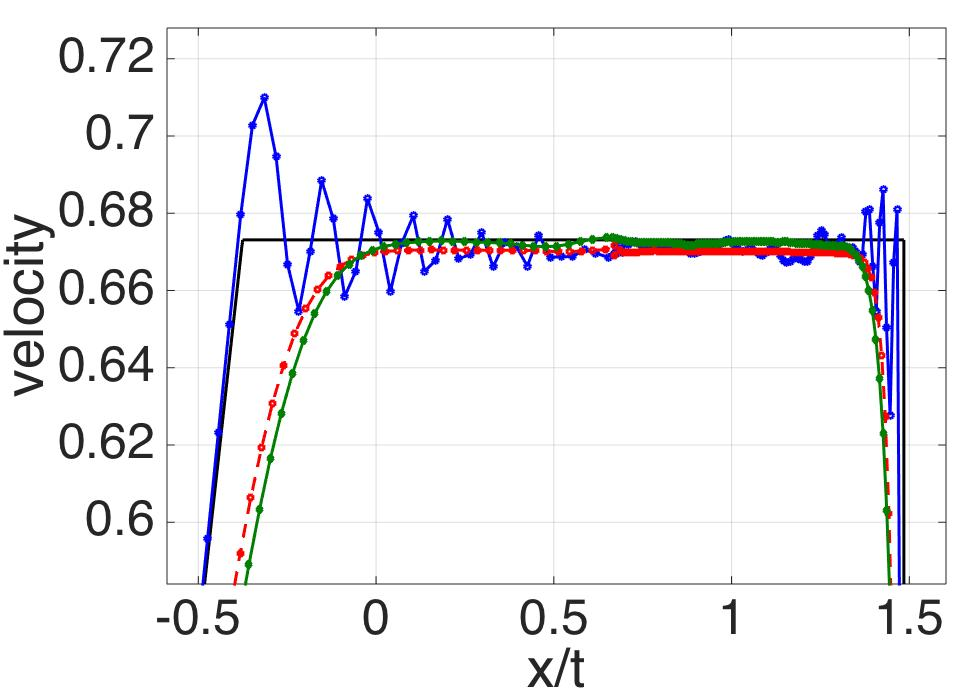
\includegraphics[width= 0.8174 \textwidth, height=0.4954 \textwidth]{./Figures/RCM-Sod-GSPH-compare-v-zoom}    
%        \end{flushleft}
%    \end{minipage}%  
%       \\
%    \begin{minipage}{.45 \textwidth}
%        \centering g)
%        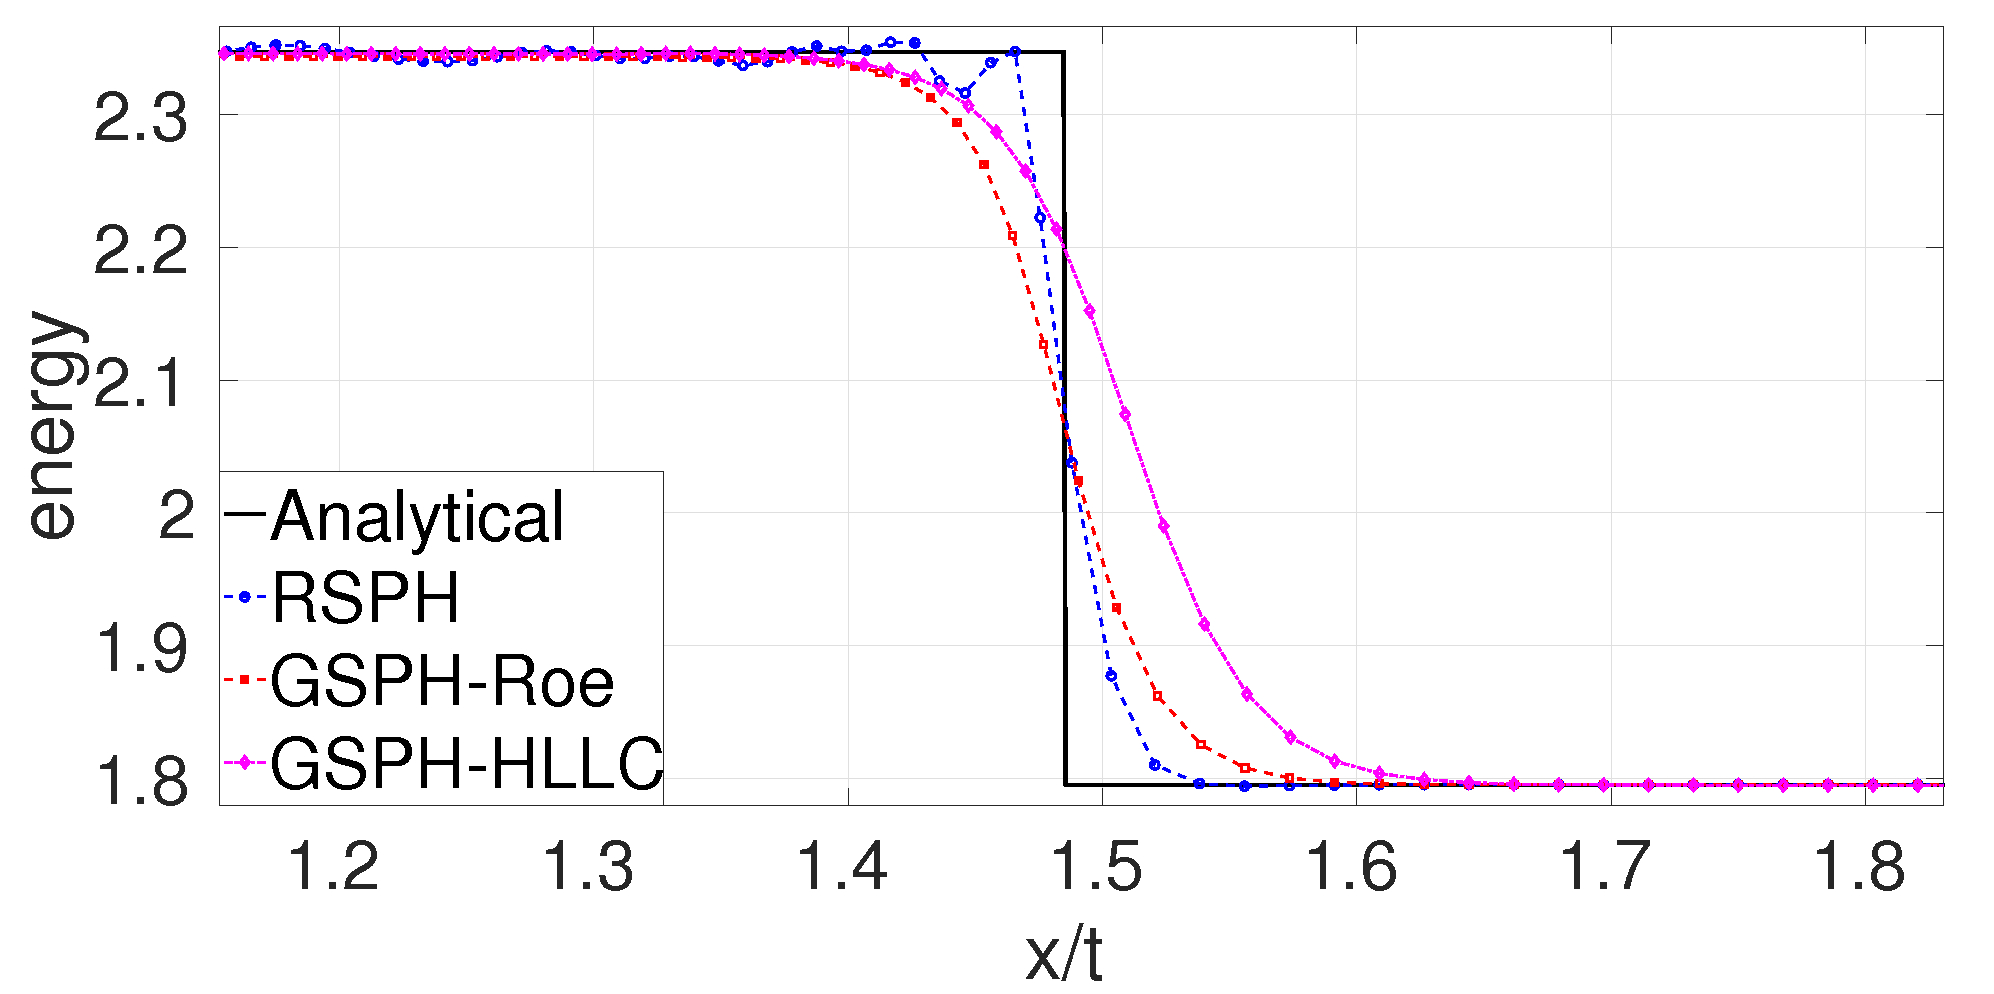
\includegraphics[width=0.99 \textwidth,height=0.6\textwidth]{./Figures/RCM-Sod-GSPH-compare-e-zoom}
%    \end{minipage}% 
%    \begin{minipage}{.545\textwidth}
%    \centering h)
%        \begin{flushleft}
%        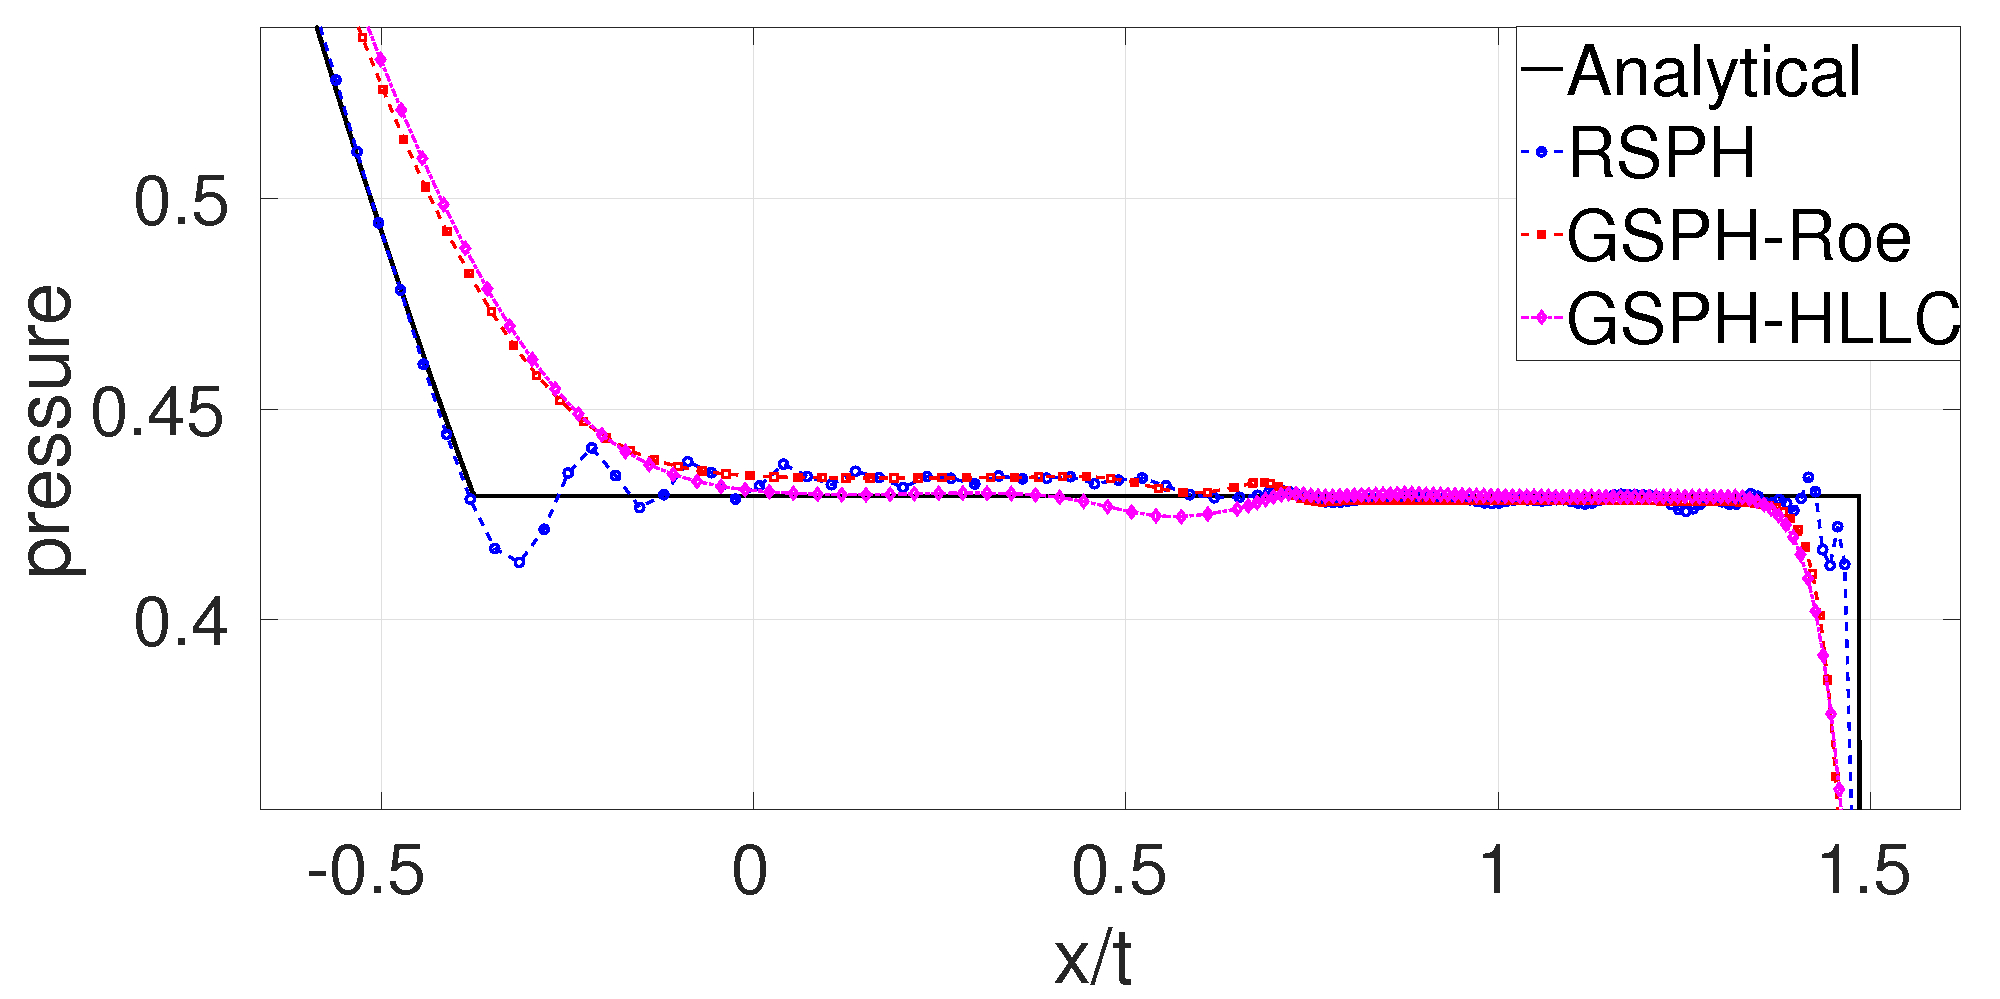
\includegraphics[width= 0.8174 \textwidth, height=0.4954 \textwidth]{./Figures/RCM-Sod-GSPH-compare-p-zoom}    
%        \end{flushleft}
%    \end{minipage}%     
    \caption{Comparison of RSPH with first order GSPH using Roe Riemann solver and HLLC Riemann solver. The last two plots are zoomed views of pressure and velocity. Zoomed view of velocity shows that fluctuation in GSPH is completely suppressed, which implies that numerical dissipation introduced in GSPH is at least around the same amount as SPH with $\alpha=1.0$. This is consistent with information implied by zoomed view of density and specific internal energy. Zoomed view of pressure shows that both RSPH and GSPH can get rid of pressure ``wiggle" around the contact discontinuity.}
    \label{fig:RCM-Sod-GSPH}
\end{figure}

RSPH is proposed to construct local Riemann problem in a piece wise constant manner while GSPH can adopt different ways for local Riemann problem construction. Besides piece wise constant construction of local Riemann problem, GSPH can also use piece wise linear construction or even higher order. In purpose of ``well-controlled" comparison, we first compare RSPH with GSPH using piece wise constant Riemann problem construction. The only difference between RSPH and piece wise constant GSPH is how to sample the solution of local Riemann problems. By such ``well-controlled" comparison, we can reveal the pure effect of random choice, the very heart of RSPH. Considering it is more popular for GSPH to construct local Riemann problem in a piece wise linear manner, we also compared RSPH with piece wise linear GSPH.

Fig. \ref{fig:RCM-Sod-GSPH} compares piece wise constant GSPH and RSPH demonstrating that RSPH introduces less but sufficient dissipation compared with piece wise constant GSPH. The attractive feature of RCM method in preserving true discontinuity is inherited by RSPH in this 1D shock tube test. With more numerical dissipation, GSPH can completely suppress numerical oscillations. However, the discontinuity at the shock is then more seriously smeared. The excessive amount of dissipation might have other, more undesirable, effects in real implementation. For example, over damping of shearing flow. Compared with SPH, both GSPH and RSPH avoid pressure ``wiggle" around contact discontinuity. Since RCM shares many commonalities with Godunov's method, it is not a surprise that RSPH can also suppress the pressure ``wiggle" at contact discontinuity.

\begin{figure}[H]
    \centering
    \begin{minipage}{.45\textwidth}
        \centering a)
        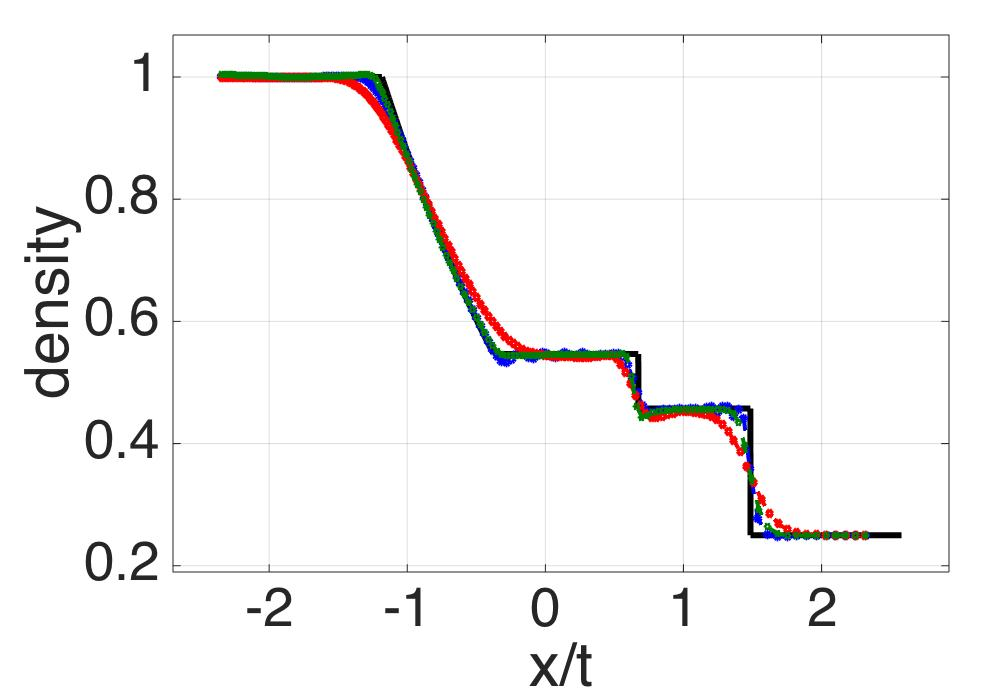
\includegraphics[width=0.99 \textwidth,height=0.6\textwidth]{./Figures/RCM-Sod-GSPH2-compare-rho}
    \end{minipage}%
    \begin{minipage}{.545\textwidth}
    \centering b)
        \begin{flushleft}
        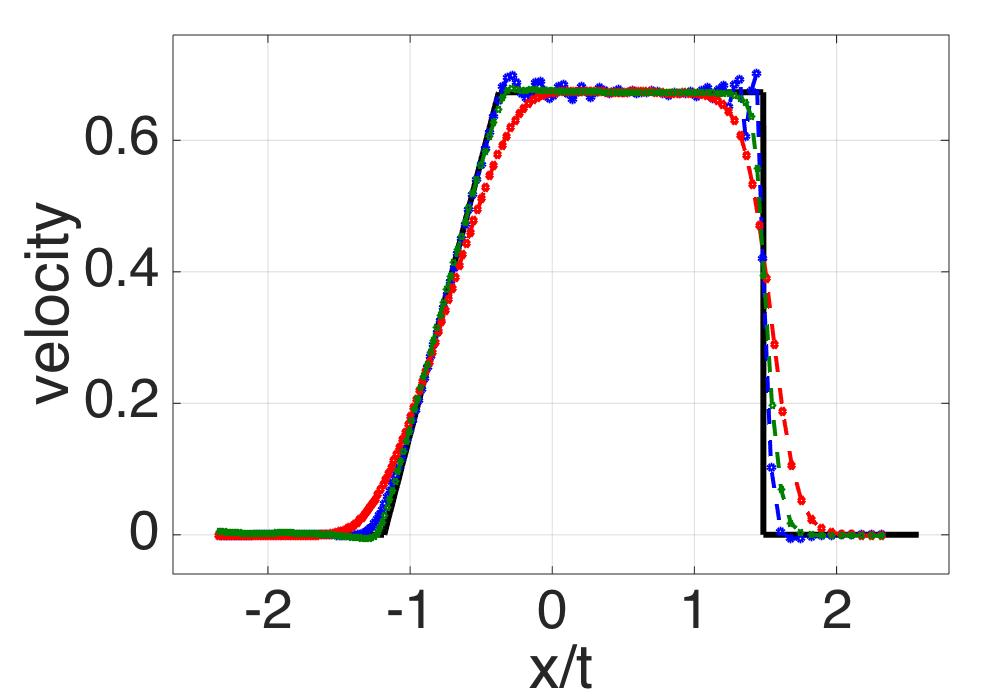
\includegraphics[width= 0.8174 \textwidth, height=0.4954 \textwidth]{./Figures/RCM-Sod-GSPH2-compare-v}    
        \end{flushleft}
    \end{minipage}% 
    \\
    \begin{minipage}{.45\textwidth}
        \centering c)
        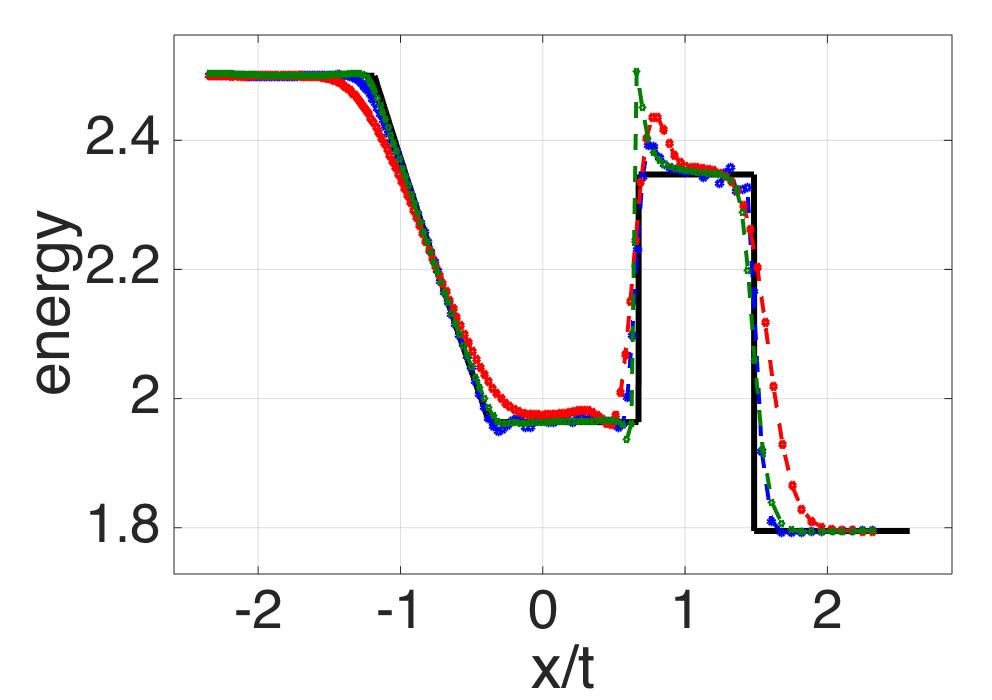
\includegraphics[width=0.99 \textwidth,height=0.6\textwidth]{./Figures/RCM-Sod-GSPH2-compare-e}
    \end{minipage}%
    \begin{minipage}{.545 \textwidth}
        \centering d)
        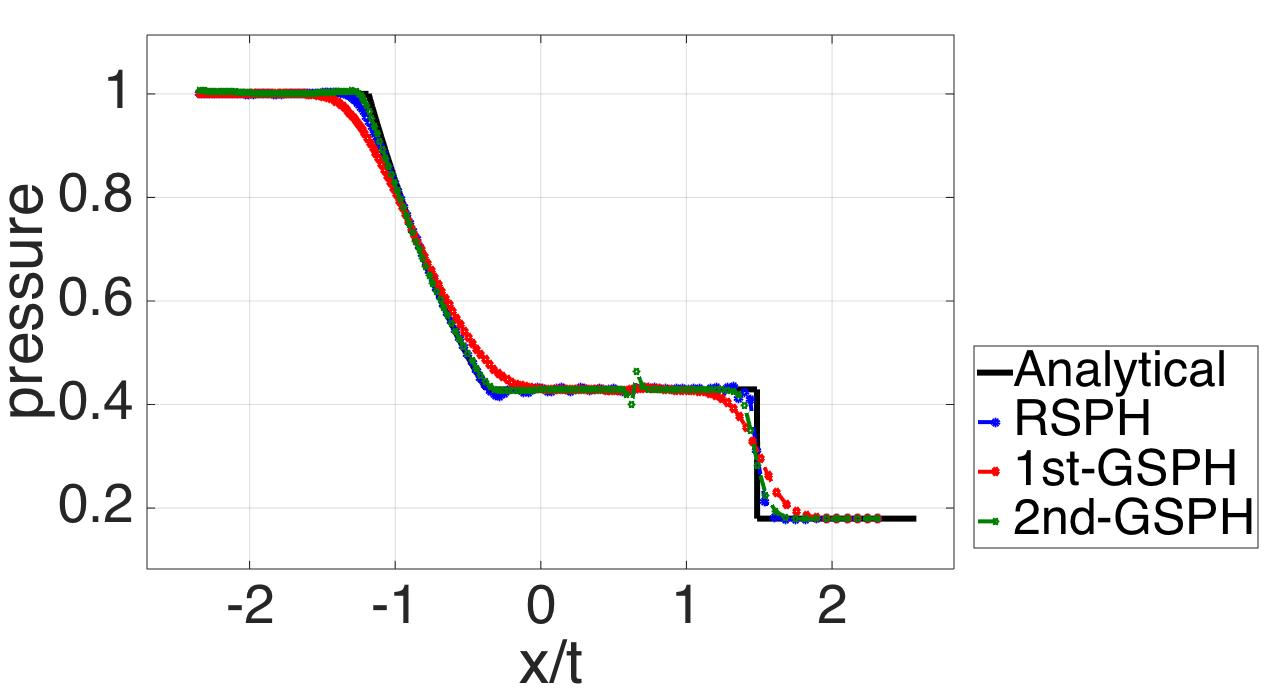
\includegraphics[width=0.99 \textwidth,height=0.4954\textwidth]{./Figures/RCM-Sod-GSPH2-compare-p}
    \end{minipage}% 
    \\
    \begin{minipage}{.45\textwidth}
        \centering e)
        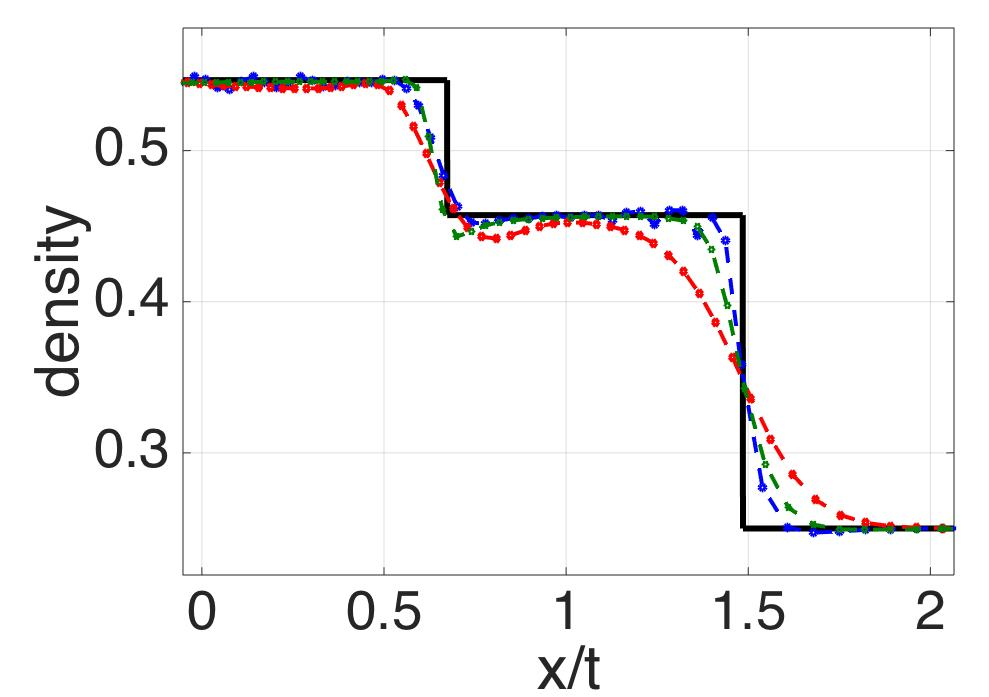
\includegraphics[width=0.99 \textwidth,height=0.6\textwidth]{./Figures/RCM-Sod-GSPH2-compare-rho-zoom}
    \end{minipage}%
    \begin{minipage}{.545\textwidth}
    \centering f)
        \begin{flushleft}
        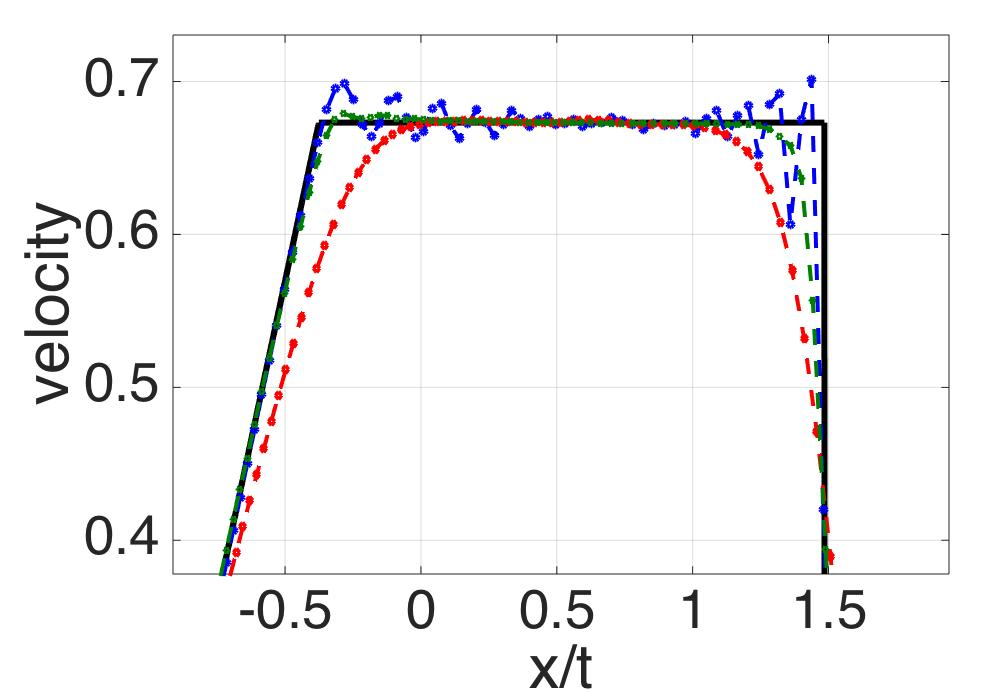
\includegraphics[width= 0.8174 \textwidth, height=0.4954 \textwidth]{./Figures/RCM-Sod-GSPH2-compare-v-zoom}    
        \end{flushleft}
    \end{minipage}%  
%       \\
%    \begin{minipage}{.45 \textwidth}
%        \centering g)
%        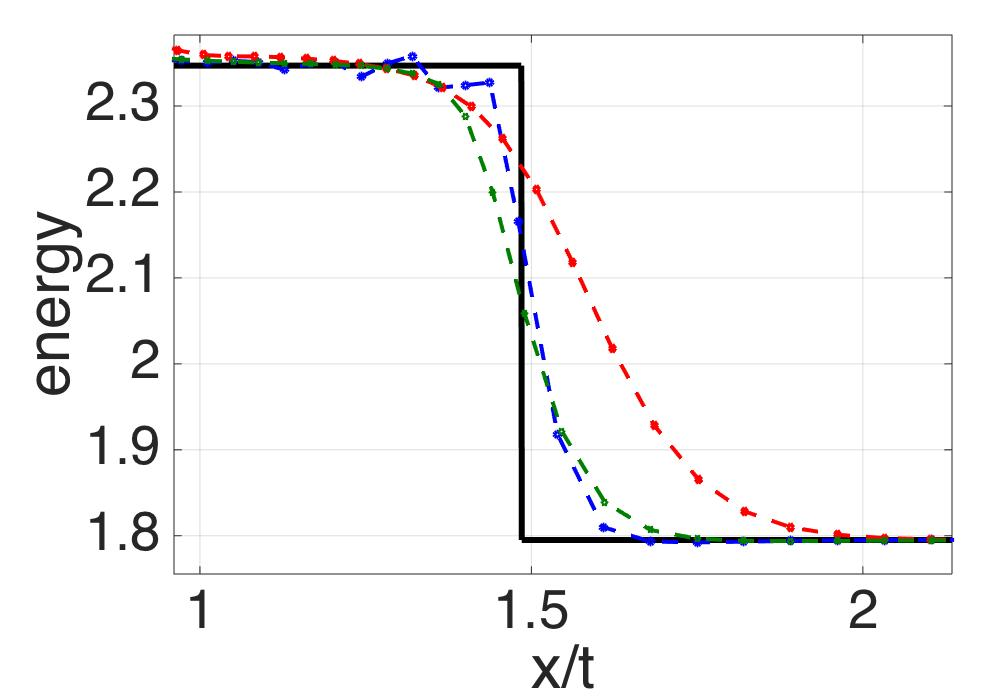
\includegraphics[width=0.99 \textwidth,height=0.6\textwidth]{./Figures/RCM-Sod-GSPH2-compare-e-zoom}
%    \end{minipage}% 
%    \begin{minipage}{.545\textwidth}
%    \centering h)
%        \begin{flushleft}
%        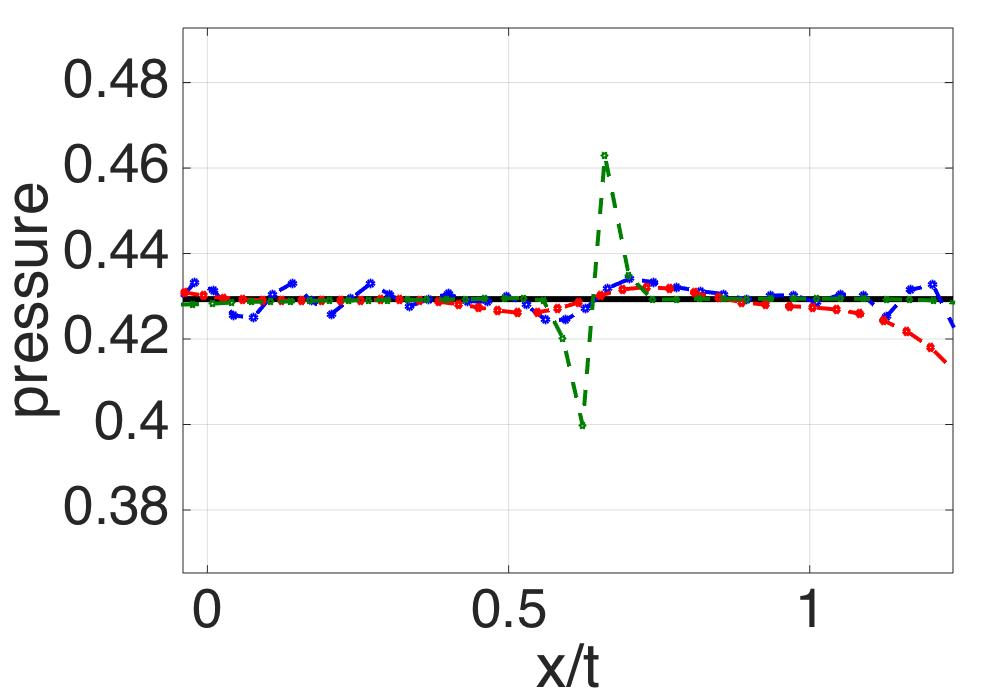
\includegraphics[width= 0.8174 \textwidth, height=0.4954 \textwidth]{./Figures/RCM-Sod-GSPH2-compare-p-zoom}    
%        \end{flushleft}
%    \end{minipage}%     
    \caption{Comparison of RSPH against GSPH with different local Riemann problem construction. Riemann problem for RSPH is constructed in a piece wise constant manner while those for GSPH are constructed in either piece wise constant manner (``1st-GSPH") or piece wise linear manner (``2nd-GSPH"). All methods adopt HLLC Riemann solver. The last two plots are zoomed views of a) and b). ``2nd-GSPH" shows better solution than ``1st-GSPH", which is just as expected. Compared with RSPH, ``2nd-GSPH" obtains almost as good results as RSPH. But there is still visible that more smearing at the shock is introduce by ``2nd-GSPH" than RSPH.}
    \label{fig:RCM-Sod-GSPH2}
\end{figure}

It is more common for GSPH to construct local Riemann problems in a piece wise linear manner. Fig. \ref{fig:RCM-Sod-GSPH2} RSPH and piece wise linear GSPH. As expected, when using higer order local Riemann problem construction, better solutions are obtained. Adopting piece wise linear Riemann problem construction reduces the amount of dissipation and hence smearing of the shocks. RSPH, even though is based on piece wise constant Riemann problem construction, still introduces less numerical dissipation than GSPH using piece wise linear Riemann problem construction. The piece wise linear Riemann problem construction requires calculation of first order derivatives while the piece wise constant manner does not. That is to say, the piece wise constant manner is computationally less expensive than the piece wise linear manner. As a consequence, RSPH would be, at least a little bit, computationally less expensive than piece wise linear GSPH.

\subsection{Accuracy tests}
We use shock tube test to gauge the accuracy of the RSPH scheme.
We examine the errors between simulation results and the analytical solution (the reference solution) as the number of particles is increased. The $L_1$ norm error, defined for a property $f$, is normalized by the number of particles as:
\begin{equation}
L_1= \frac{1}{N_p} \sum_a^{N_p} \vert f_a^{SPH} - f^{REF} (x_a) \vert 
\end{equation}
where the superscript $REF$ represent the reference solution, $SPH$ represents simulation results calculated by different SPH schemes. Fig. \ref{fig:Accuracy-test1} displays the $L_1$ norm errors for the density, velocity and pressure profiles for different SPH schemes.

Due to symmetry of kernel function, estimation of density (Eq. (\ref{eq:ns-sph-d})) in SPH can reach second order of accuracy if all particles distribute in space with uniform interval. However, such ideal situation is very rare. Due to irregular particle distribution, we usually observe order of accuracy between 1 and 2. Besides the particle distribution in space, which has major affect on order of accuracy of SPH, some other aspects would also influence order of accuracy. For SPH schemes that depend on solving Riemann problems, how the local Riemann problem is constructed also influence order of accuracy. 
For GSPH, the Riemann problem can be constructed in piece wise constant manner, piece wise linear manner or even higher order \citep{inutsuka2002reformulation}. For RSPH, we can only consider to construct local Riemann problems in the piece wise constant manner. When using other higher order construction of local Riemann problem, how to determine the range for ``random choice" is not clear. This is a limitation of current RSPH compared with GSPH. With simper Riemann problem construction, RSPH is expected to be faster than GSPH adopting higher order Riemann problem construction. To compare RSPH and GSPH in a well-controlled manner, all GSPH tests presented in this paper are based on piece wise constant construction of local Riemann problems.

We observe a rate of convergence of approximately 1 for GSPH and 1.5 for standard SPH and RSPH.  Considering Riemann problem is constructed in piece wise constant manner, it is not surprise that GSPH shows first order of accuracy. With piece wise linear construction of Riemann problem, GSPH would be higher order of accuracy. For example,
GSPH combined with HLLC and Roe approximate Riemann solvers has been shown to be approximately second order of accuracy \citep{puri2014comparison} and comparable in accuracy to the standard SPH schemes when construct local Riemann problem in a piece wise linear manners. Presence of discontinuities, such as shock, in the test problem might lead to more irregular distribution of particles and lower the rate of convergence. 

Since both RSPH and GSPH tests in this paper adopt the same manner for Riemann problem construction. We conclude that RSPH shows higher order of accuracy than GSPH providing both use the same Riemann problem construction. Compared with SPH, RSPH shows almost the same order of accuracy and level of error.
 
\begin{figure}[H]
    \centering
    \begin{minipage}{.30\textwidth}
        \centering
        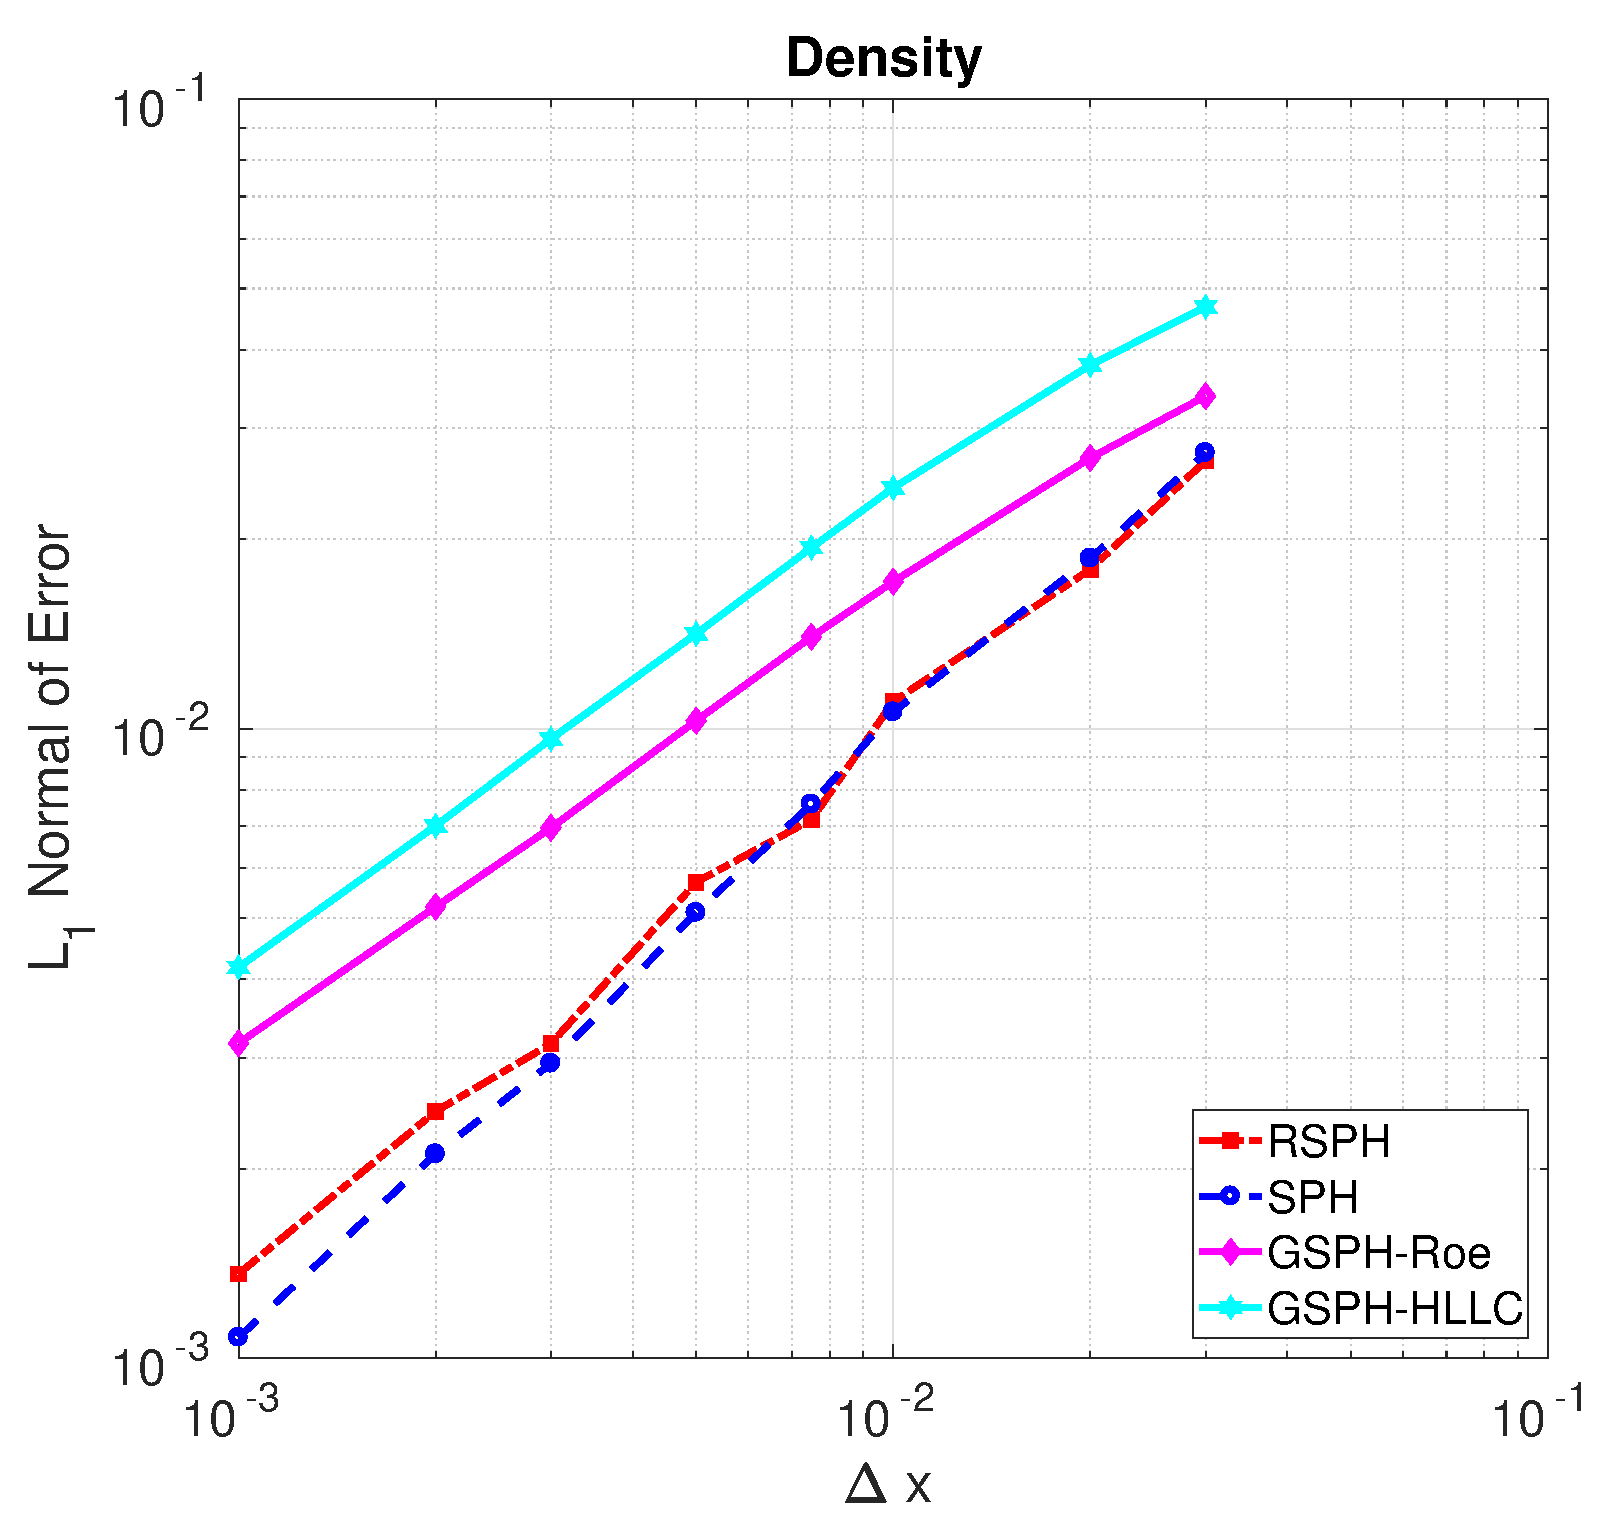
\includegraphics[width=0.99 \textwidth]{./Figures/Accuracy-des}
    \end{minipage}%
    \begin{minipage}{.30 \textwidth}
        \centering
        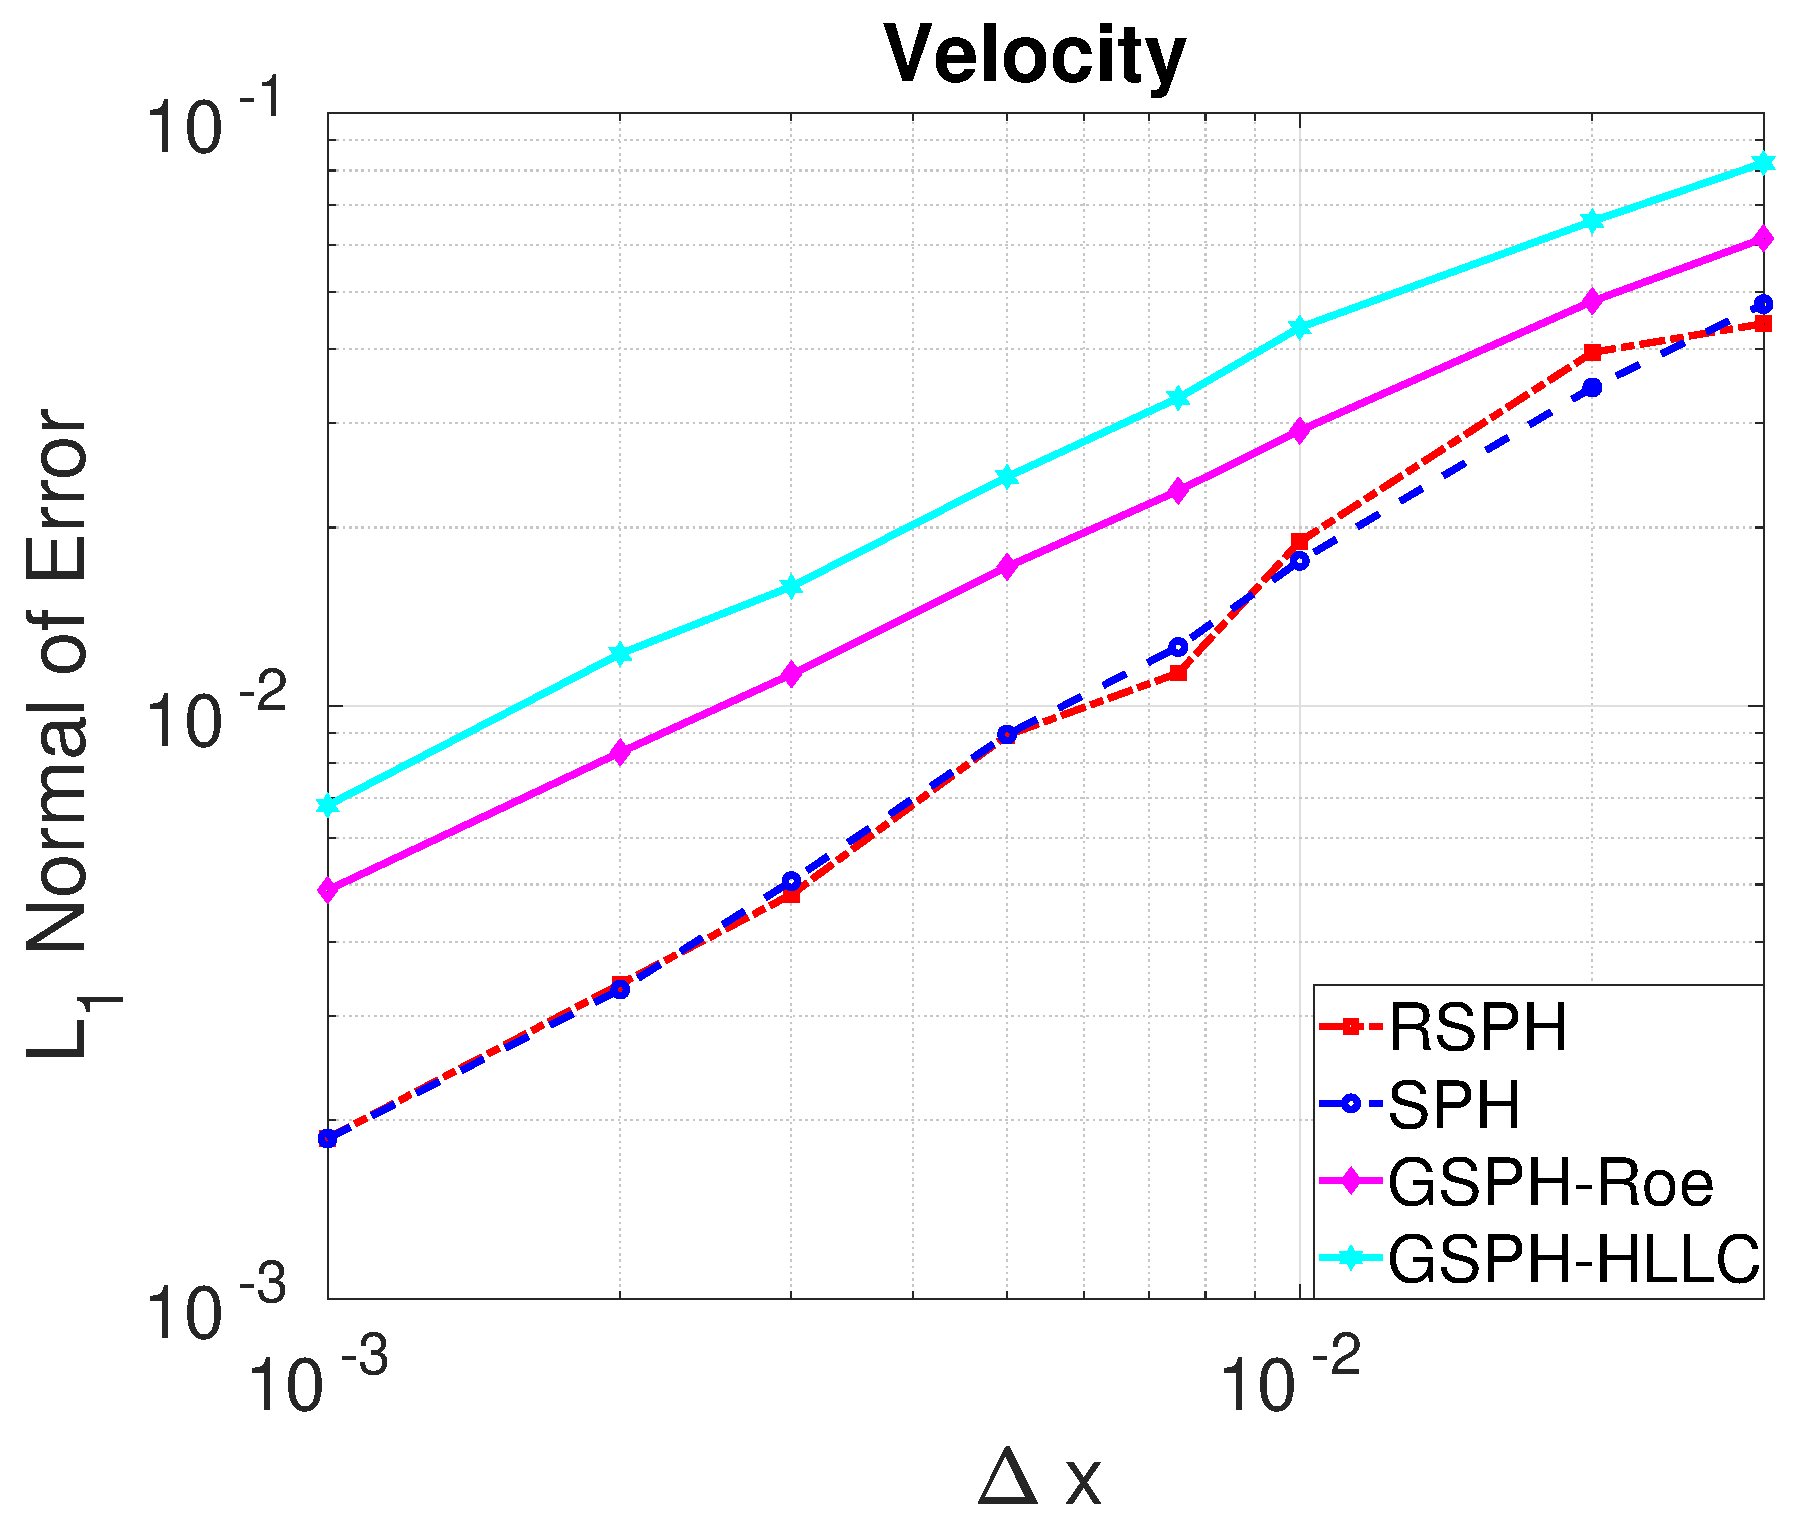
\includegraphics[width=0.99 \textwidth]{./Figures/Accuracy-vel}
    \end{minipage}%
    \begin{minipage}{.39\textwidth}
        \centering
        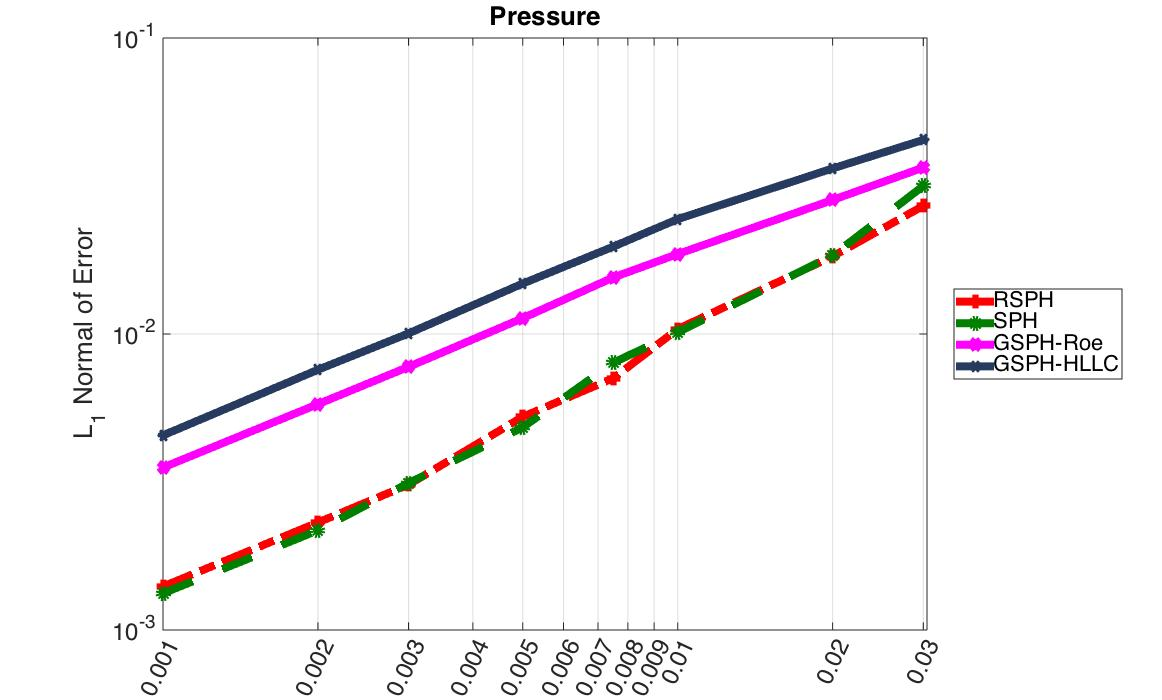
\includegraphics[width=0.99 \textwidth]{./Figures/Accuracy-pre}
    \end{minipage}%  
    \caption{ $L_1$ norm of errors for 1D shock tube test (test1) for RSPH, standard SPH, GSPH using Roe Riemann solver and GSPH using HLLC Riemann Solver. GSPH with the HLLC approximate Riemann solver exhibits the same convergence rate (around 1) but quantitatively larger errors than that with Roe Riemann solver. RSPH and standard SPH shows same rate of convergence and almost same level of error.}
    \label{fig:Accuracy-test1}
\end{figure}
 
\subsection{Comprehensive 1D tests} \label{sec:comprehensive-1d-tests}
Comprehensive tests are presented in this section to check how well does RSPH work for different wave patterns. Input parameters for each tests is given in Table \ref{tab:1D-shock-input_parameters}.
The results are shown in Fig. \ref{fig:RCM-GSPH-Sod} $\sim$ Fig. \ref{fig:RCM-strong-blast}. $x$ axis in these plots are normalized by the terminal time $t_f$. 
We observe that RSPH is able to correctly predict the position and magnitude of all waves for all tests. A jump of specific internal energy at the origin is observed in Sj$\ddot{o}$green test. However, such jump is a common issue of SPH schemes and has been reported in many other tests (see, for example, \citep{monaghan1997sph,cha2003implementations,puri2014approximate})
In addition, a noticeable spike can be observed near the contact discontinuity. Similar spike is observed in GSPH simulation \citep{puri2014comparison}.
\citet{noh1987errors} proposed to adding a small amount of thermal conduction to ameliorate the spike and has been applied in blast-wave test using GSPH \citep{puri2014comparison}. We did not adopt such strategy in our simulation.
Due to less amount of dissipation, the numerical oscillations, which is due to nonuniform smoothing length as discussed in Appendix B, persist in all simulation results. For the strong blast test and double shock test, such oscillation becomes more obvious than other tests, even though, the magnitude of fluctuations is within an acceptable range.

\begin{figure}[H]
    \centering
    \begin{minipage}{.415\textwidth}
        \centering
        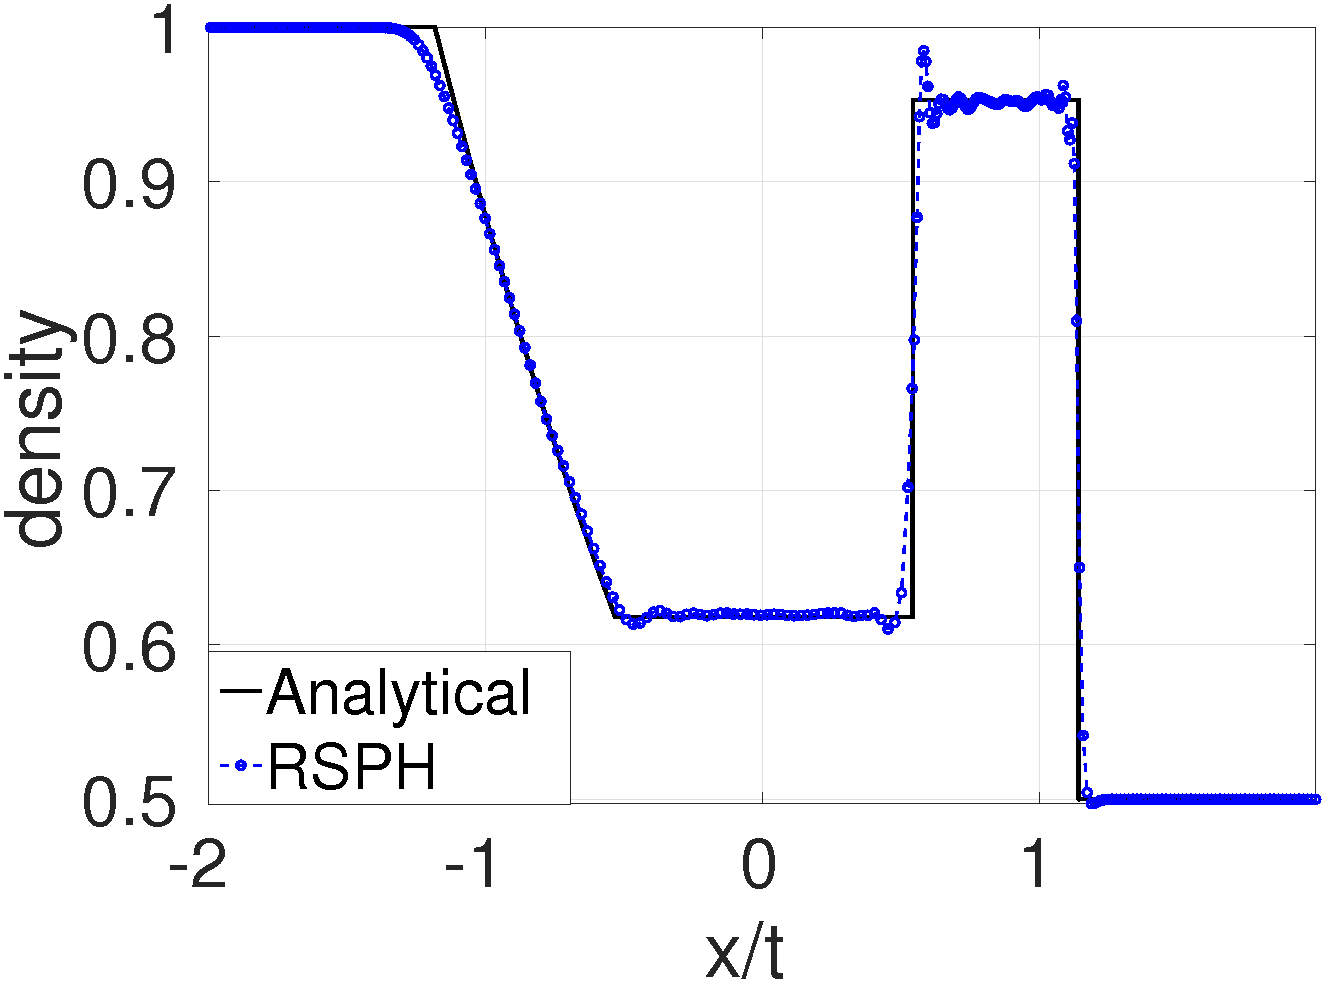
\includegraphics[width=0.99 \textwidth]{./Figures/GRod-RCM-rho}
    \end{minipage}%
    \begin{minipage}{.512 \textwidth}
        \begin{flushleft}
        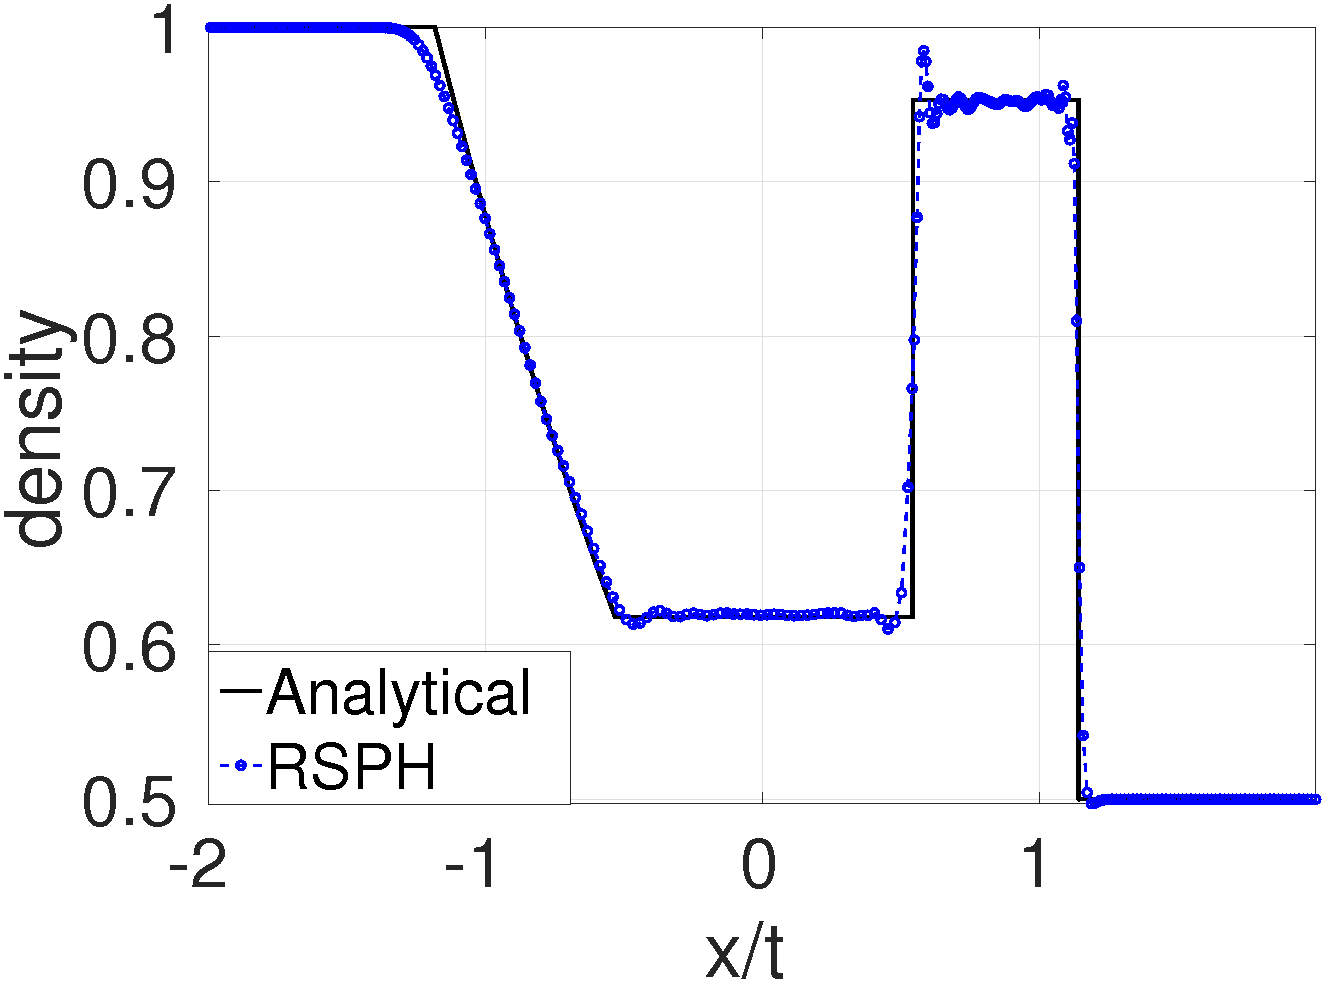
\includegraphics[width=0.8024 \textwidth]{./Figures/GRod-RCM-rho}
        \end{flushleft}
    \end{minipage}%    
    \\
    \begin{minipage}{.415\textwidth}
        \centering
        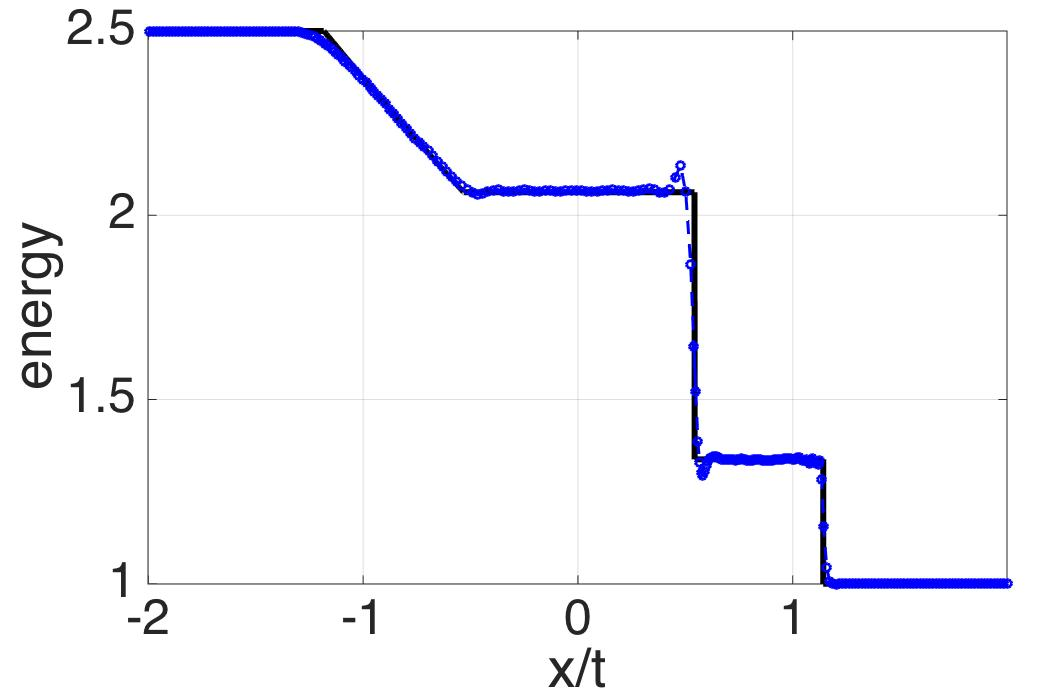
\includegraphics[width=0.99 \textwidth]{./Figures/GRod-RCM-e}
    \end{minipage}%
    \begin{minipage}{.512 \textwidth}
        \centering
        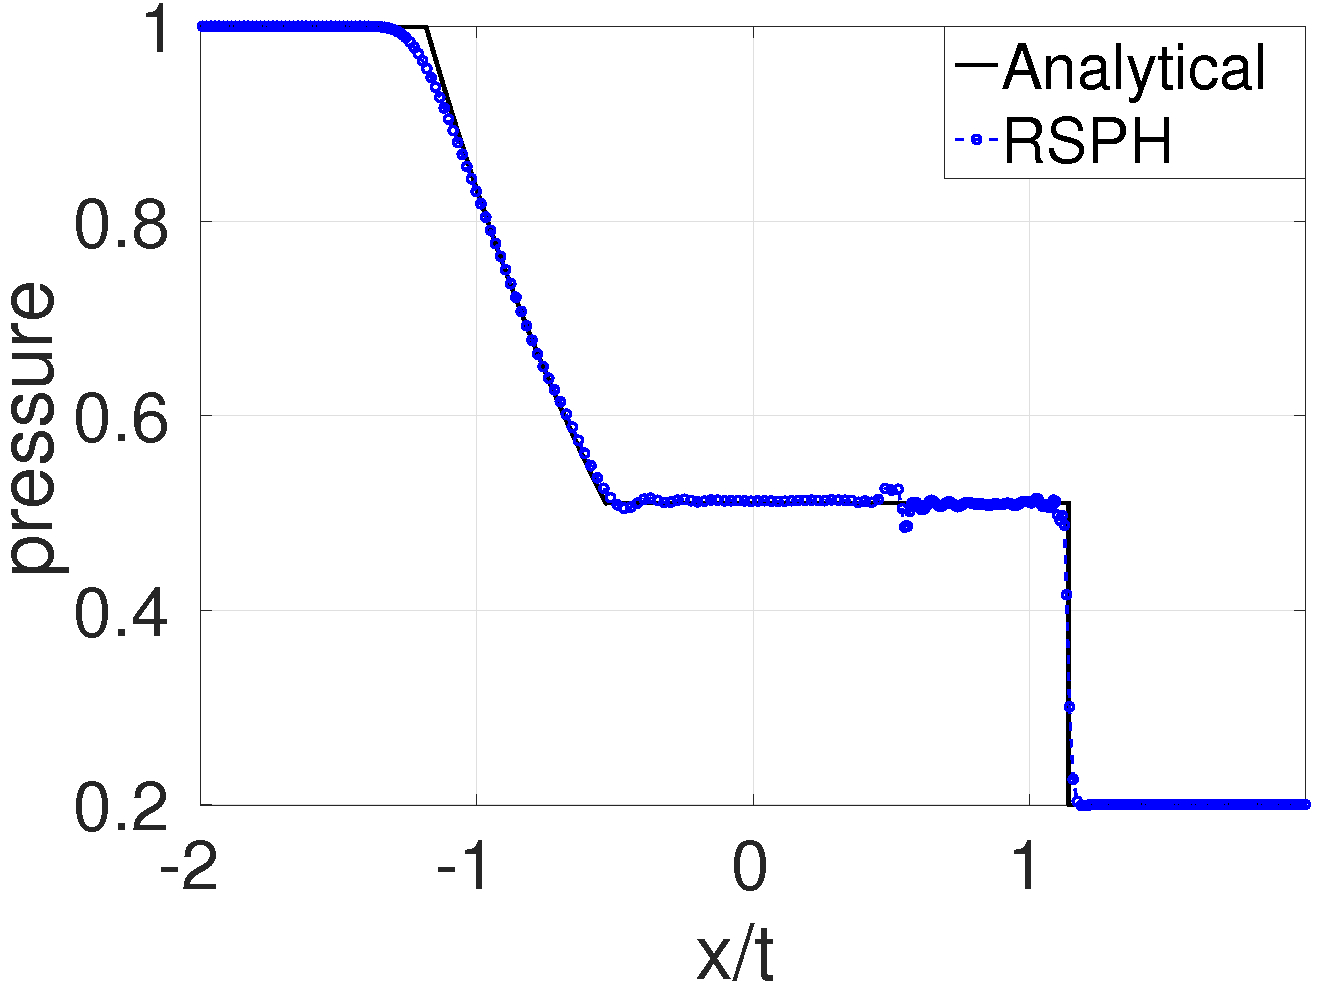
\includegraphics[width=0.99 \textwidth]{./Figures/GRod-RCM-p}
    \end{minipage}% 
    \caption{Results for test 2, a variation of Sod test. All physical properties are well re-produced except for some acceptable oscillations}
    \label{fig:RCM-GSPH-Sod}
\end{figure}

\begin{figure}[H]
    \centering
    \begin{minipage}{.415\textwidth}
        \centering
        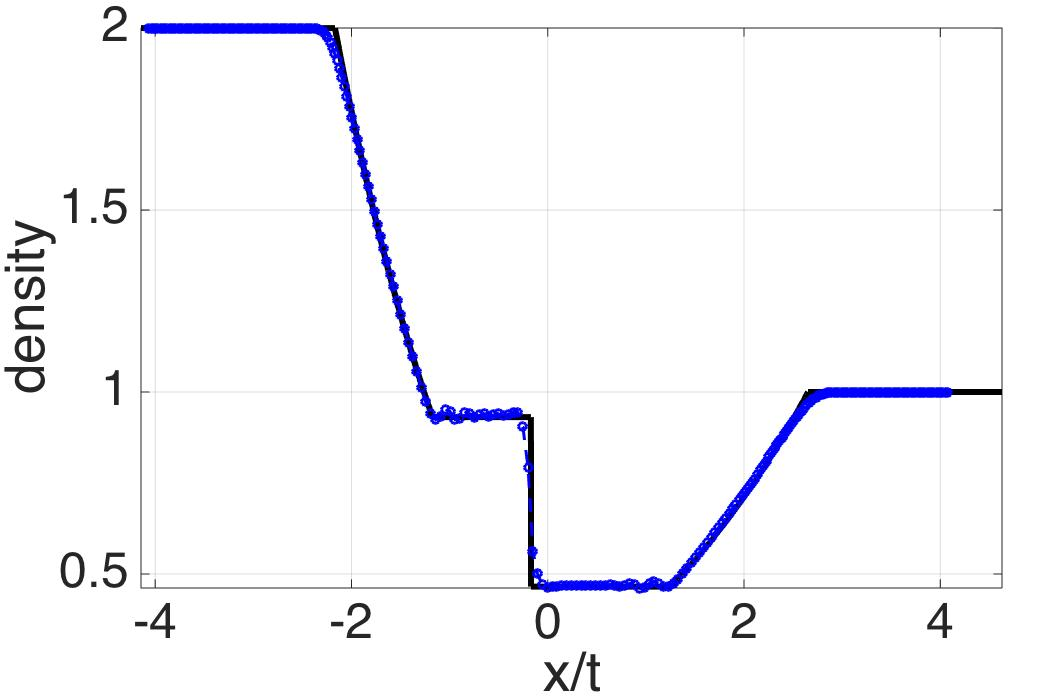
\includegraphics[width=0.99 \textwidth]{./Figures/Dexp-RCM-rho}
    \end{minipage}%
    \begin{minipage}{.512 \textwidth}
        \begin{flushleft}
        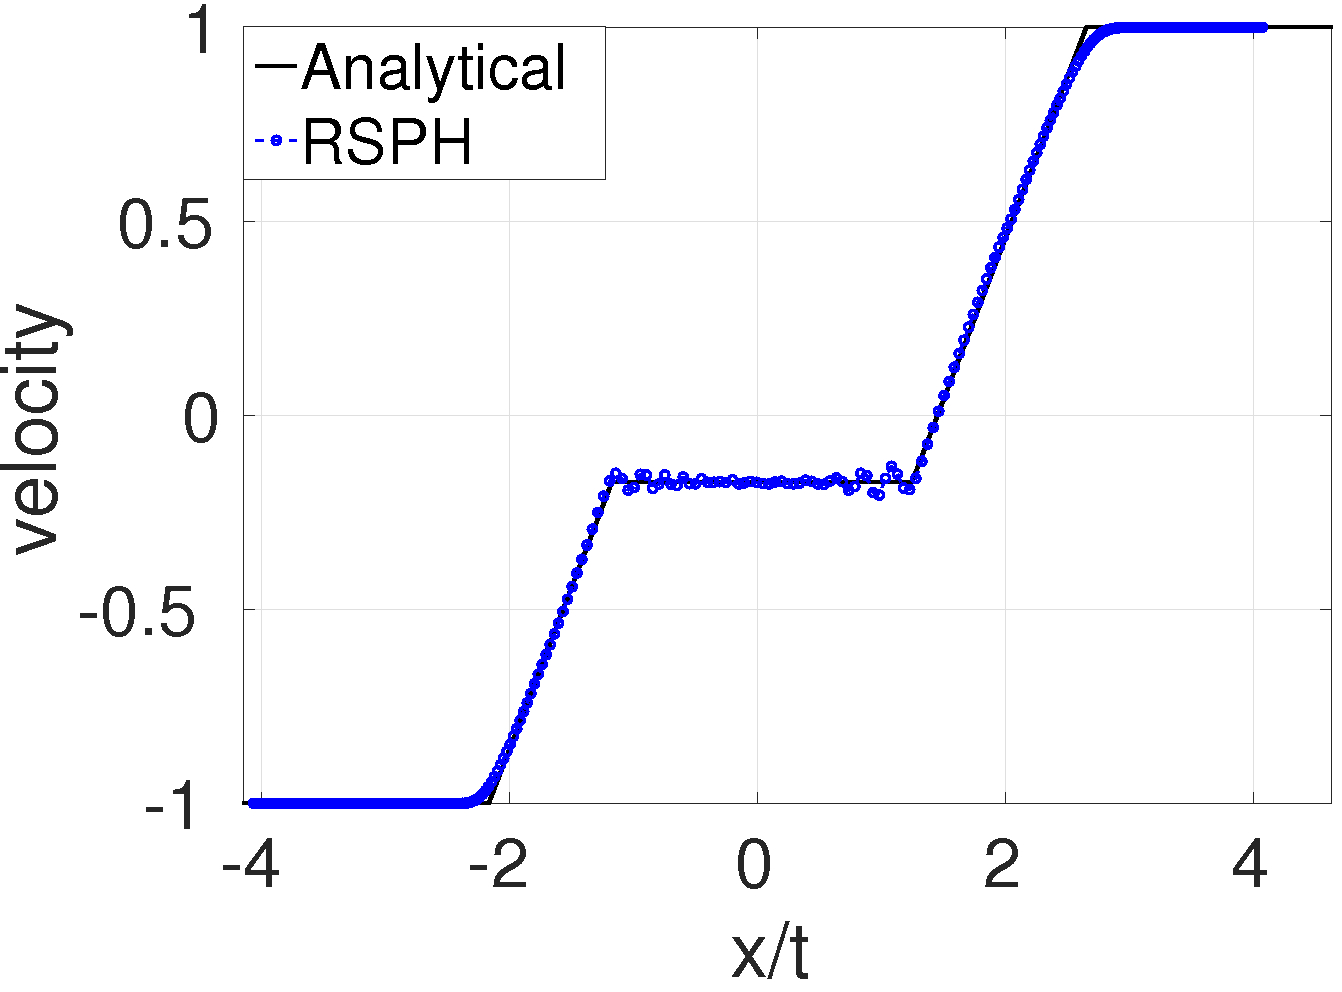
\includegraphics[width=0.8024 \textwidth]{./Figures/Dexp-RCM-v}
        \end{flushleft}
    \end{minipage}%     
    \\
    \begin{minipage}{.415\textwidth}
        \centering
        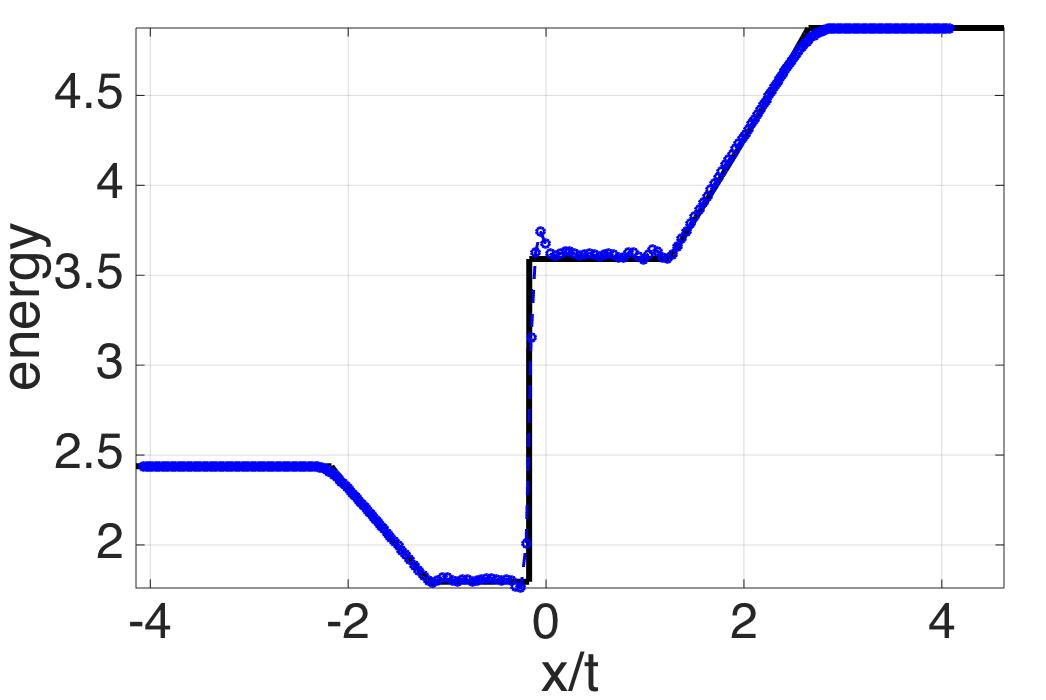
\includegraphics[width=0.99 \textwidth]{./Figures/Dexp-RCM-e}
    \end{minipage}%
    \begin{minipage}{.512 \textwidth}
        \centering
        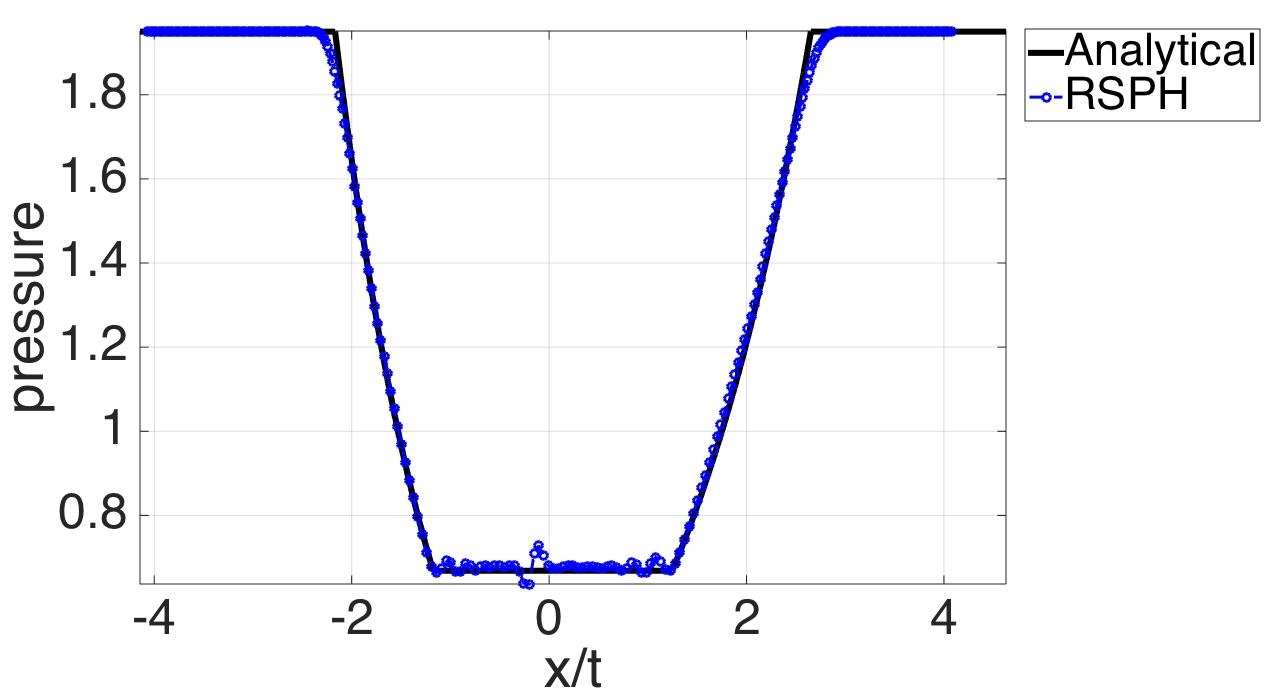
\includegraphics[width=0.99 \textwidth]{./Figures/Dexp-RCM-p}
    \end{minipage}% 
    \caption{Results for test 3, the double expansion case. All physical properties are well re-produced except for some oscillations}
    \label{fig:RCM-double-expansion}
\end{figure}

\begin{figure}[H]
    %\centering
    \begin{minipage}{.415\textwidth}
        \centering
        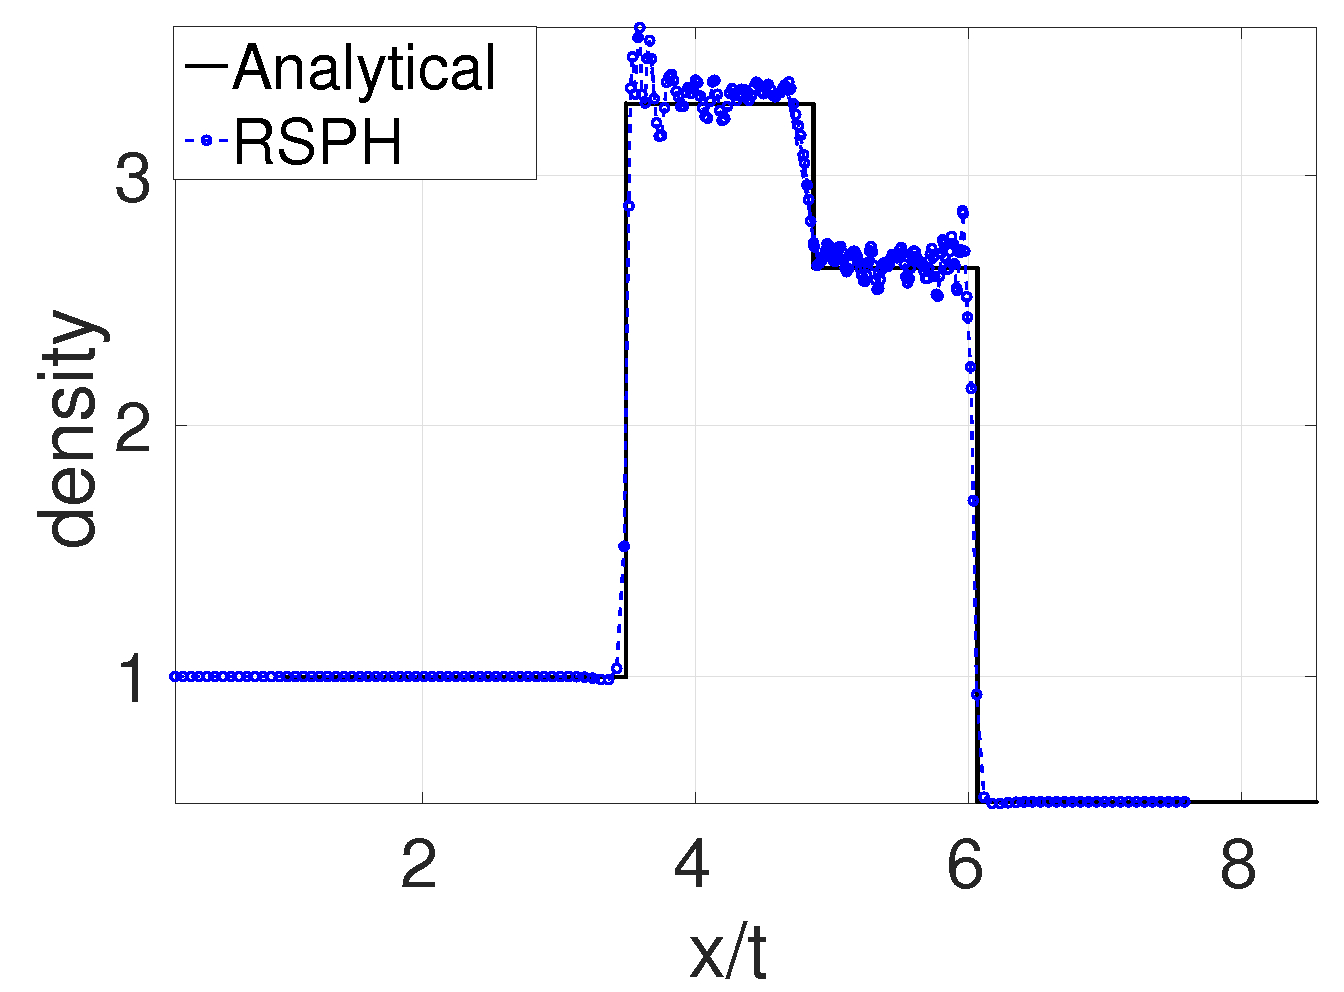
\includegraphics[width=0.99 \textwidth]{./Figures/Dshock-RCM-rho-Rp6}
    \end{minipage}%
    \begin{minipage}{.512 \textwidth}
        \begin{flushleft}
        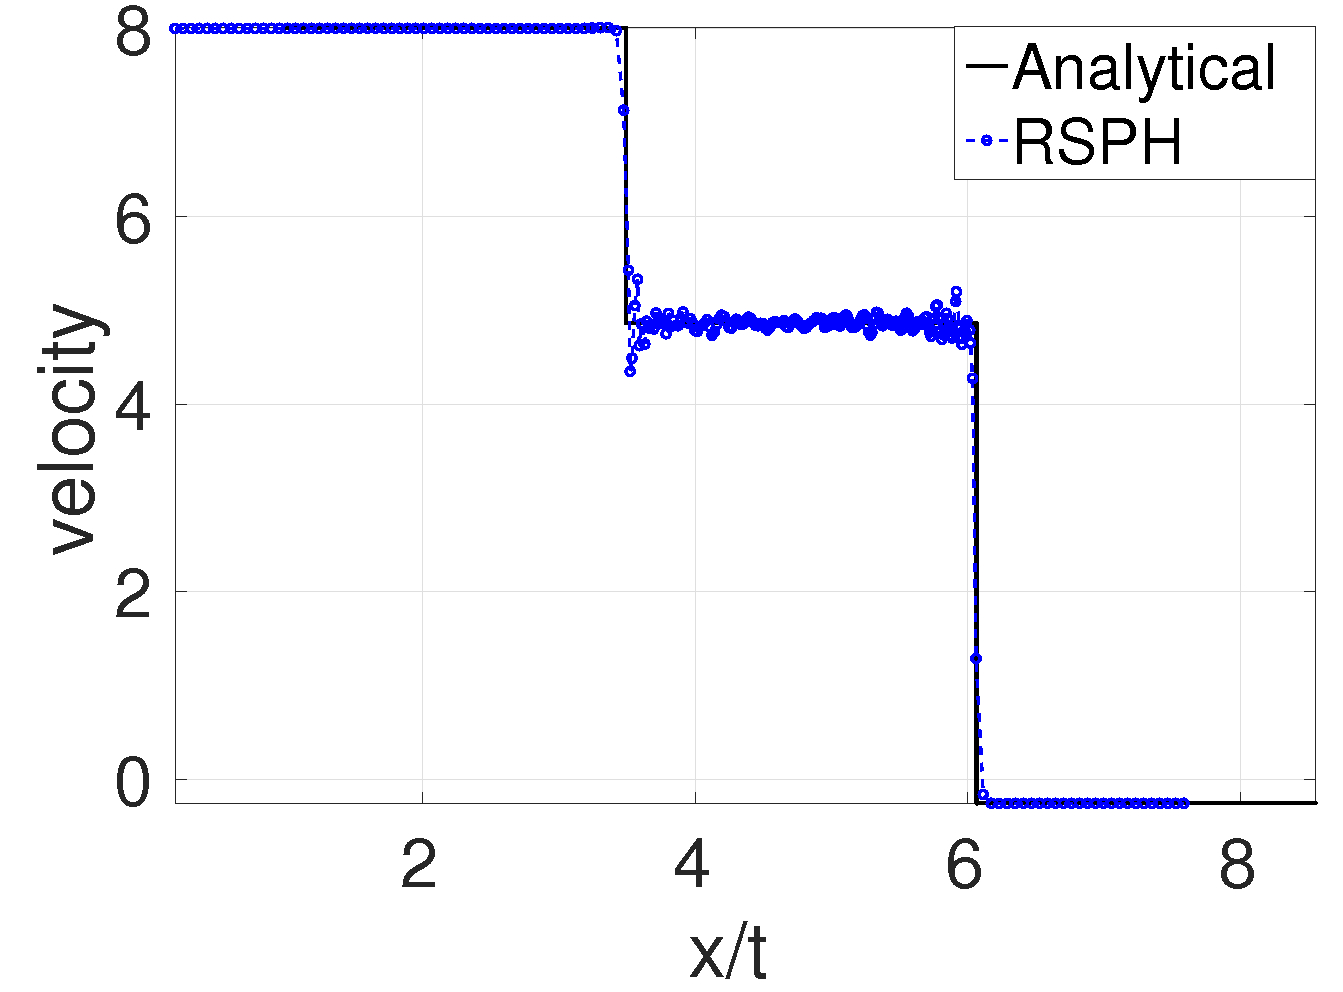
\includegraphics[width=0.8024 \textwidth]{./Figures/Dshock-RCM-v-Rp6}
        \end{flushleft}
    \end{minipage}%     
    \\
    \begin{minipage}{.415\textwidth}
        \centering
        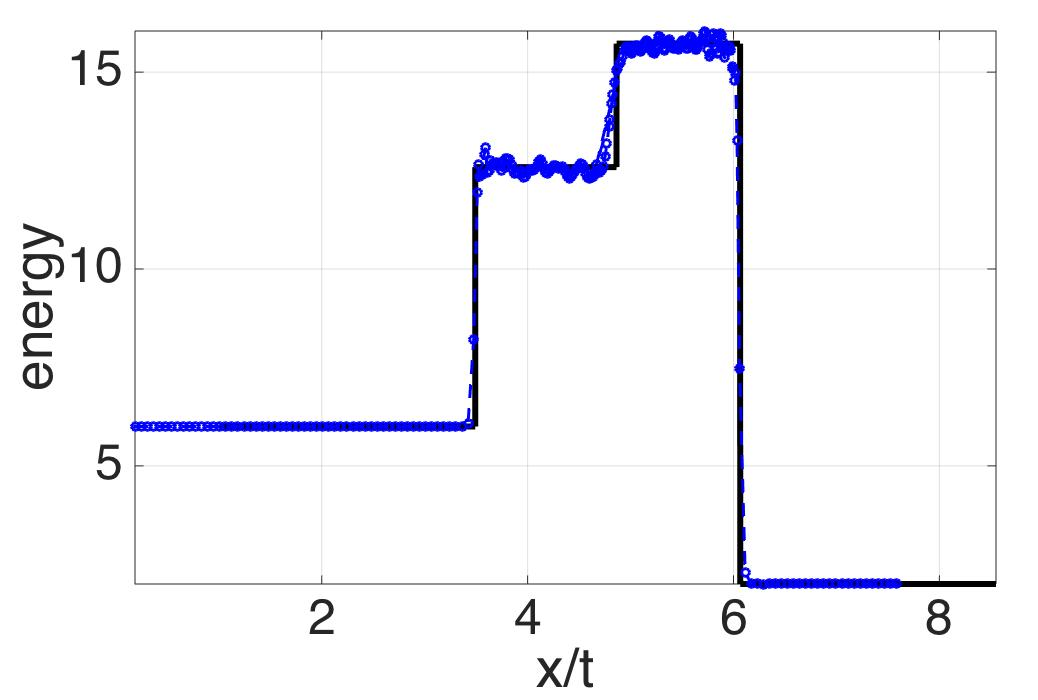
\includegraphics[width=0.99 \textwidth]{./Figures/Dshock-RCM-e-Rp6}
    \end{minipage}%
    \begin{minipage}{.512 \textwidth}
        \centering
        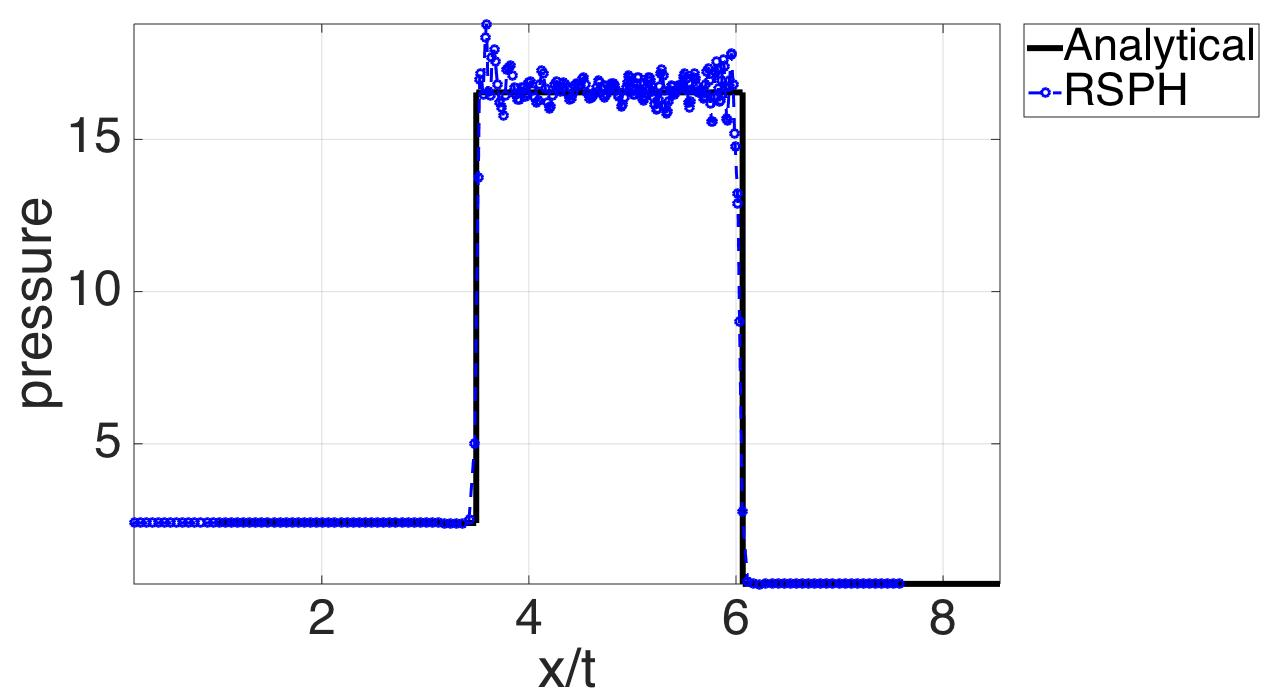
\includegraphics[width=0.99 \textwidth]{./Figures/Dshock-RCM-p-Rp6}
    \end{minipage}% 
    \caption{Results for test 4, the double shock case. To stabilize the simulation, RSPH sampling is in a narrower range. All physical properties are well re-produced. However, the oscillations are more serious than oscillations in other tests.}
    \label{fig:RCM-double-shock}
\end{figure}

\begin{figure}[H]
    \begin{minipage}{.415\textwidth}
        \centering
        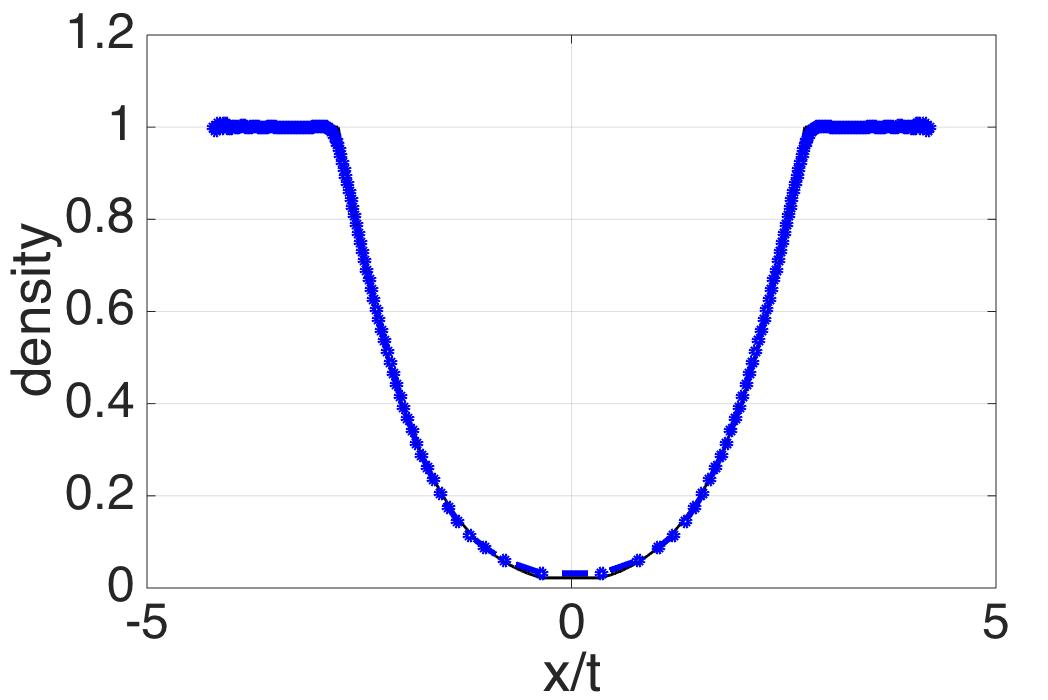
\includegraphics[width=0.99 \textwidth]{./Figures/Sjogreen-RCM-rho-Adpt1}
    \end{minipage}%
    \begin{minipage}{.512 \textwidth}
        \begin{flushleft}
        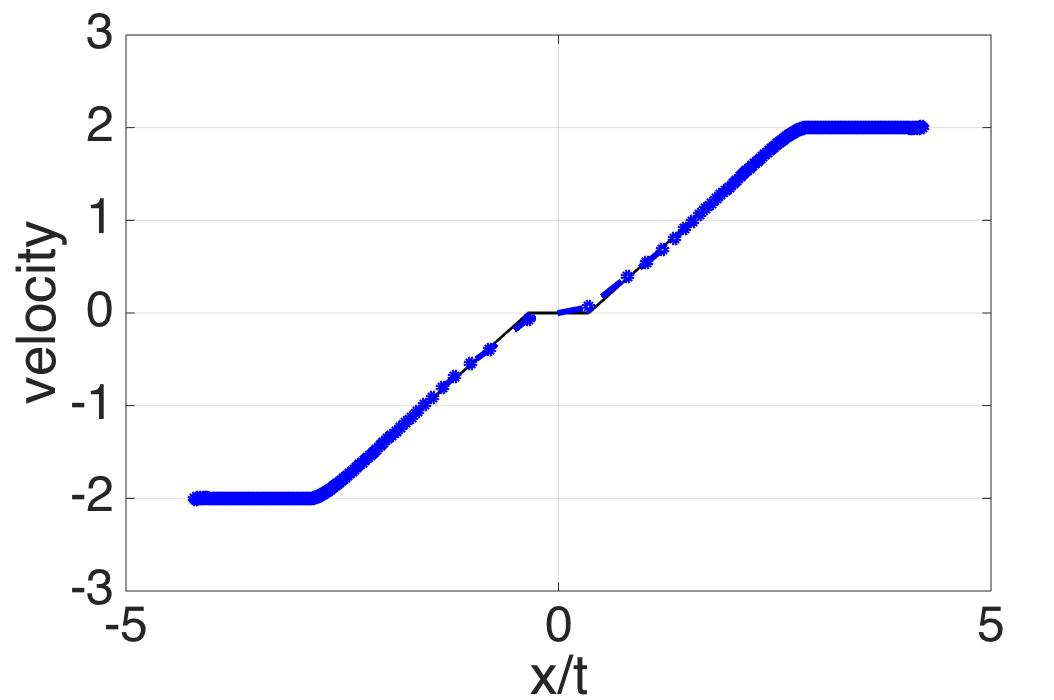
\includegraphics[width=0.8024 \textwidth]{./Figures/Sjogreen-RCM-v-Adpt1}
        \end{flushleft}
    \end{minipage}%       
    \\
    \begin{minipage}{.415\textwidth}
        \centering
        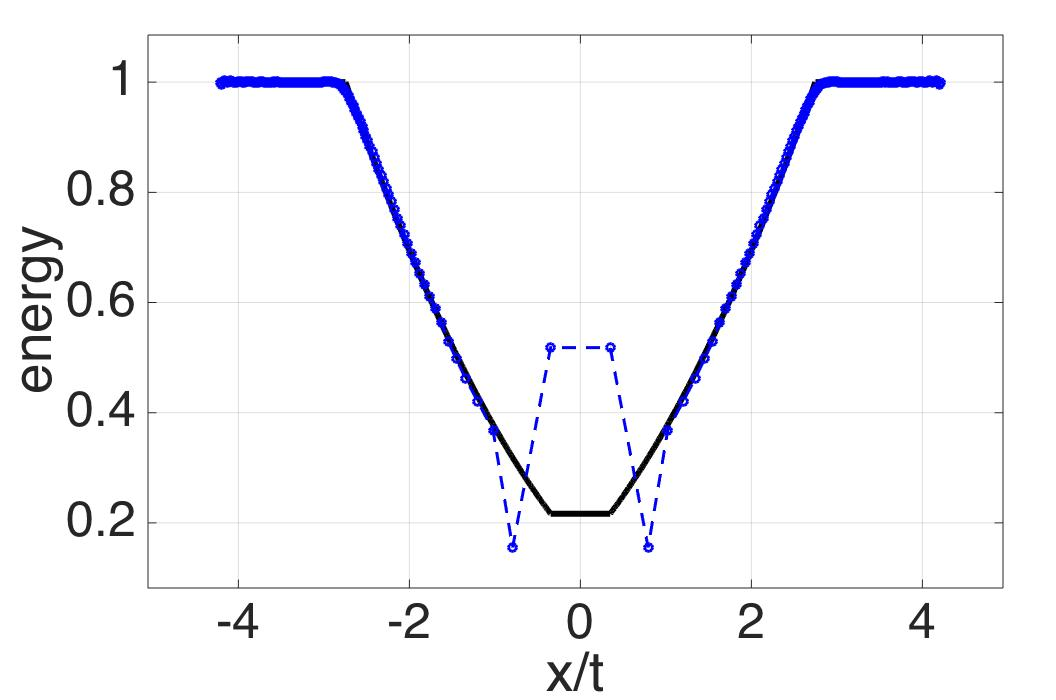
\includegraphics[width=0.99 \textwidth]{./Figures/Sjogreen-RCM-e-Adpt1}
    \end{minipage}%
    \begin{minipage}{.512 \textwidth}
        \centering
        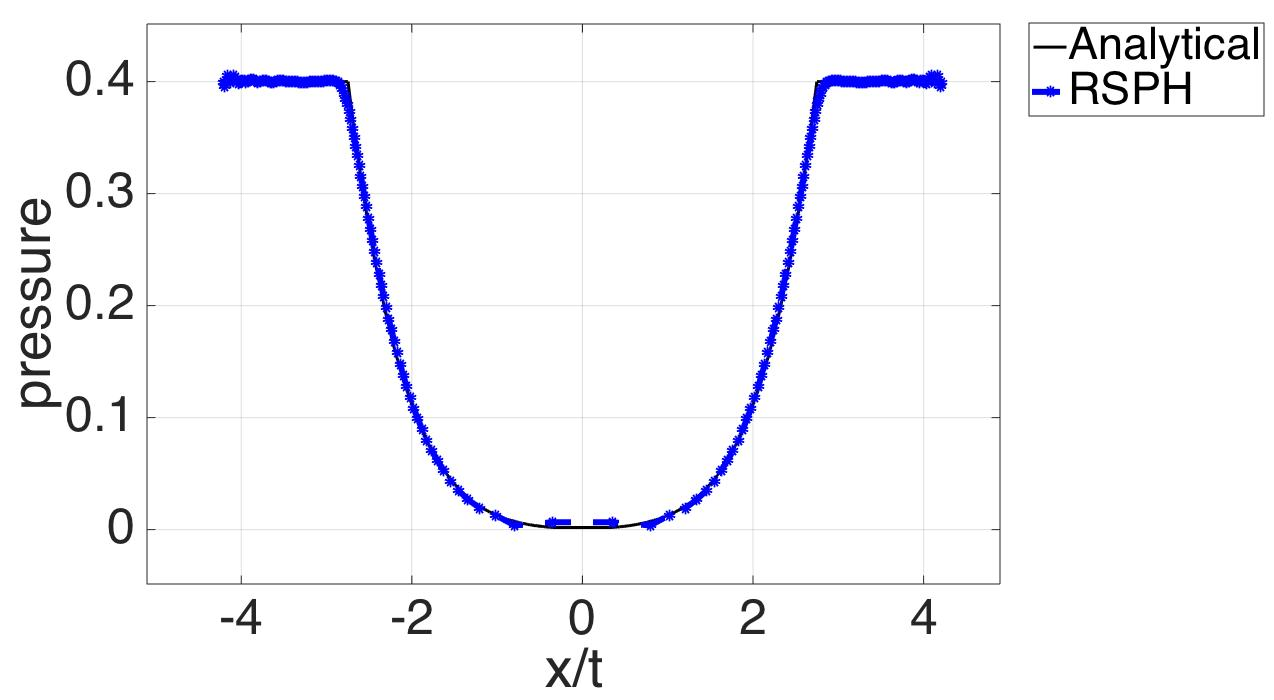
\includegraphics[width=0.99 \textwidth]{./Figures/Sjogreen-RCM-p-Adpt1}
    \end{minipage}% 
    \caption{Results for test 5, a variation of the Sj$\ddot{o}$green test. The density, velocity and pressure are well re-produced while the thermal energy at the origin is poorly predicted. A jump of internal energy at the origin is a common issue in many SPH schemes (see, for example, \citep{monaghan1997sph,cha2003implementations,puri2014approximate})}
    \label{fig:RCM-Sjogreen}
\end{figure}

\begin{figure}[H]
    \centering
    \begin{minipage}{.415\textwidth}
        \centering
        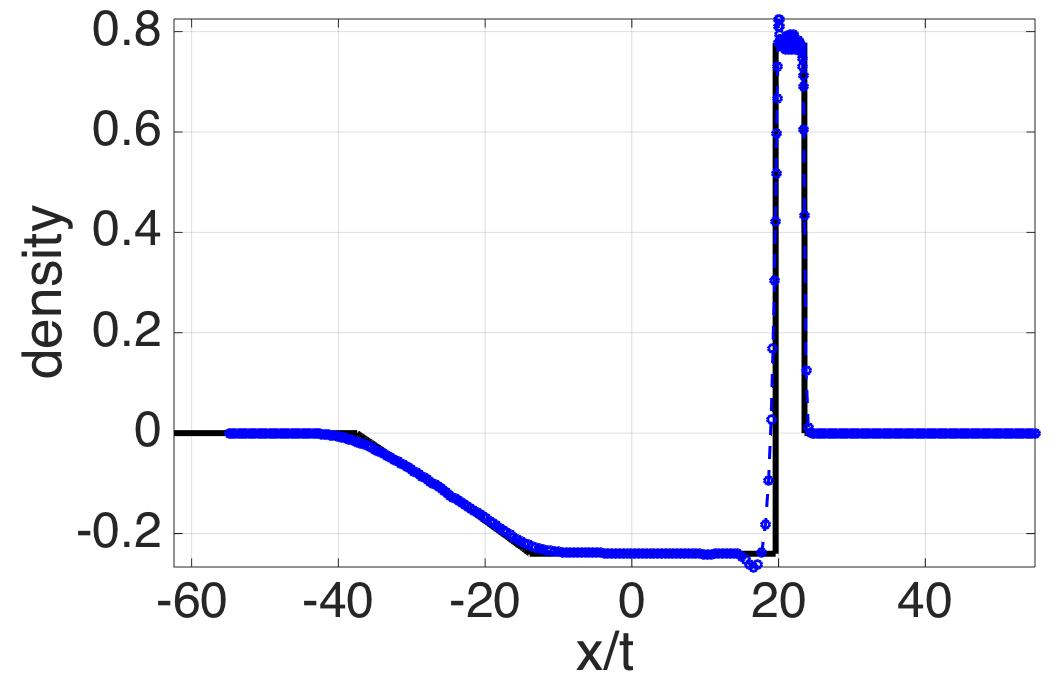
\includegraphics[width=0.99 \textwidth]{./Figures/StrBlst-RCM-rho-Rp3}
    \end{minipage}%
    \begin{minipage}{.512 \textwidth}
        \begin{flushleft}
        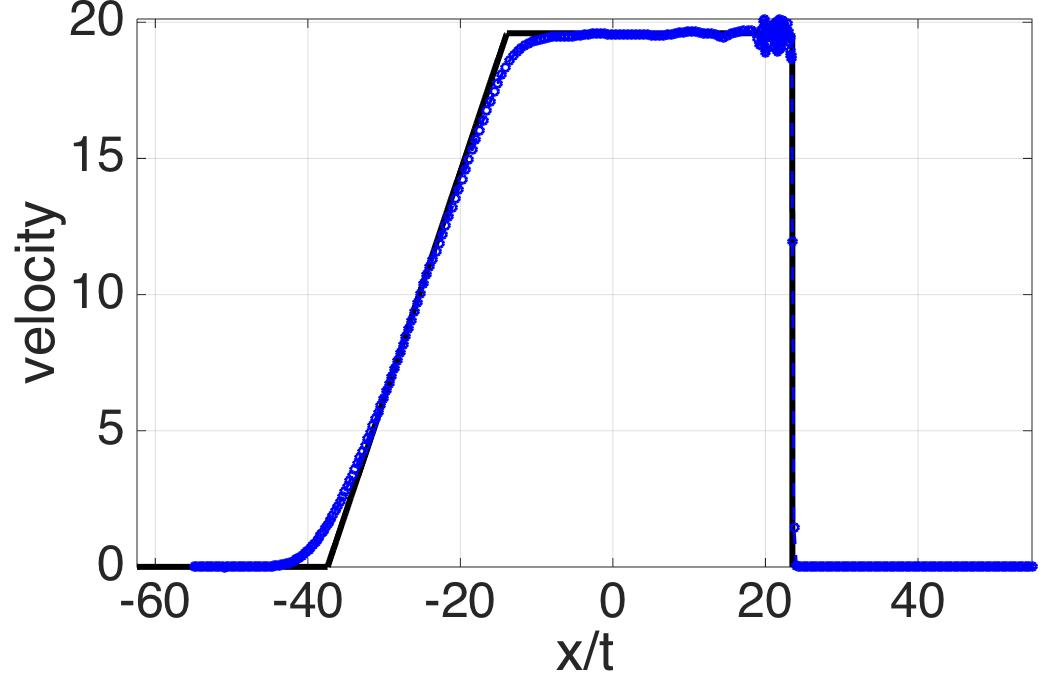
\includegraphics[width=0.8024 \textwidth]{./Figures/StrBlst-RCM-v-Rp3}
        \end{flushleft}
    \end{minipage}%
    \\
    \begin{minipage}{.415 \textwidth}
        \centering
        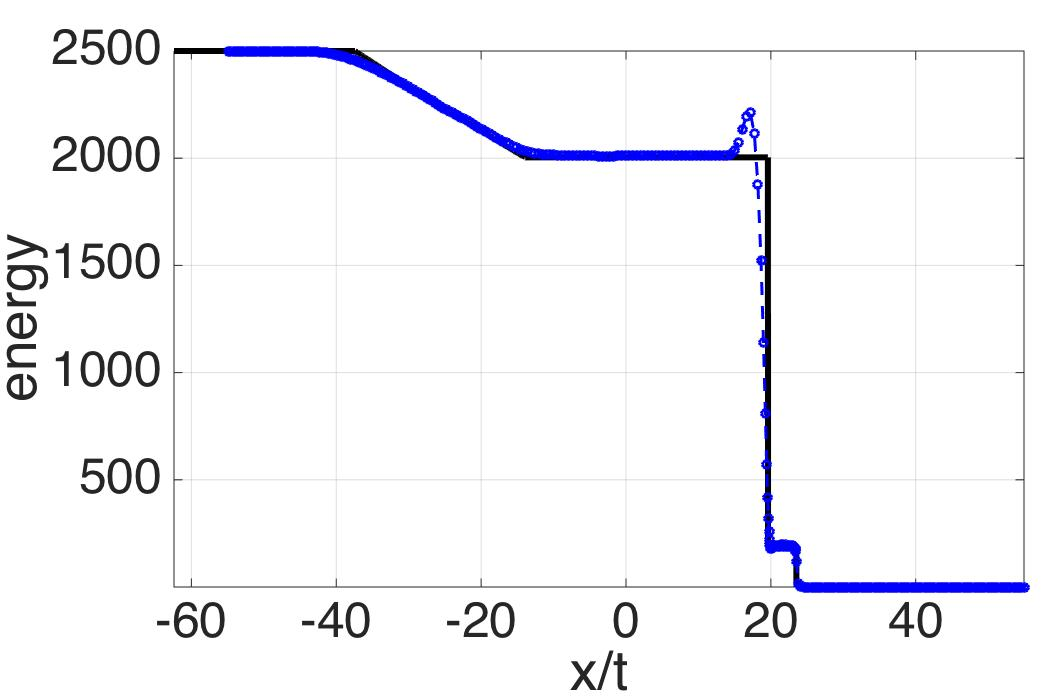
\includegraphics[width=0.99 \textwidth]{./Figures/StrBlst-RCM-e-Rp3}
    \end{minipage}%
    \begin{minipage}{.512 \textwidth}
        \centering
        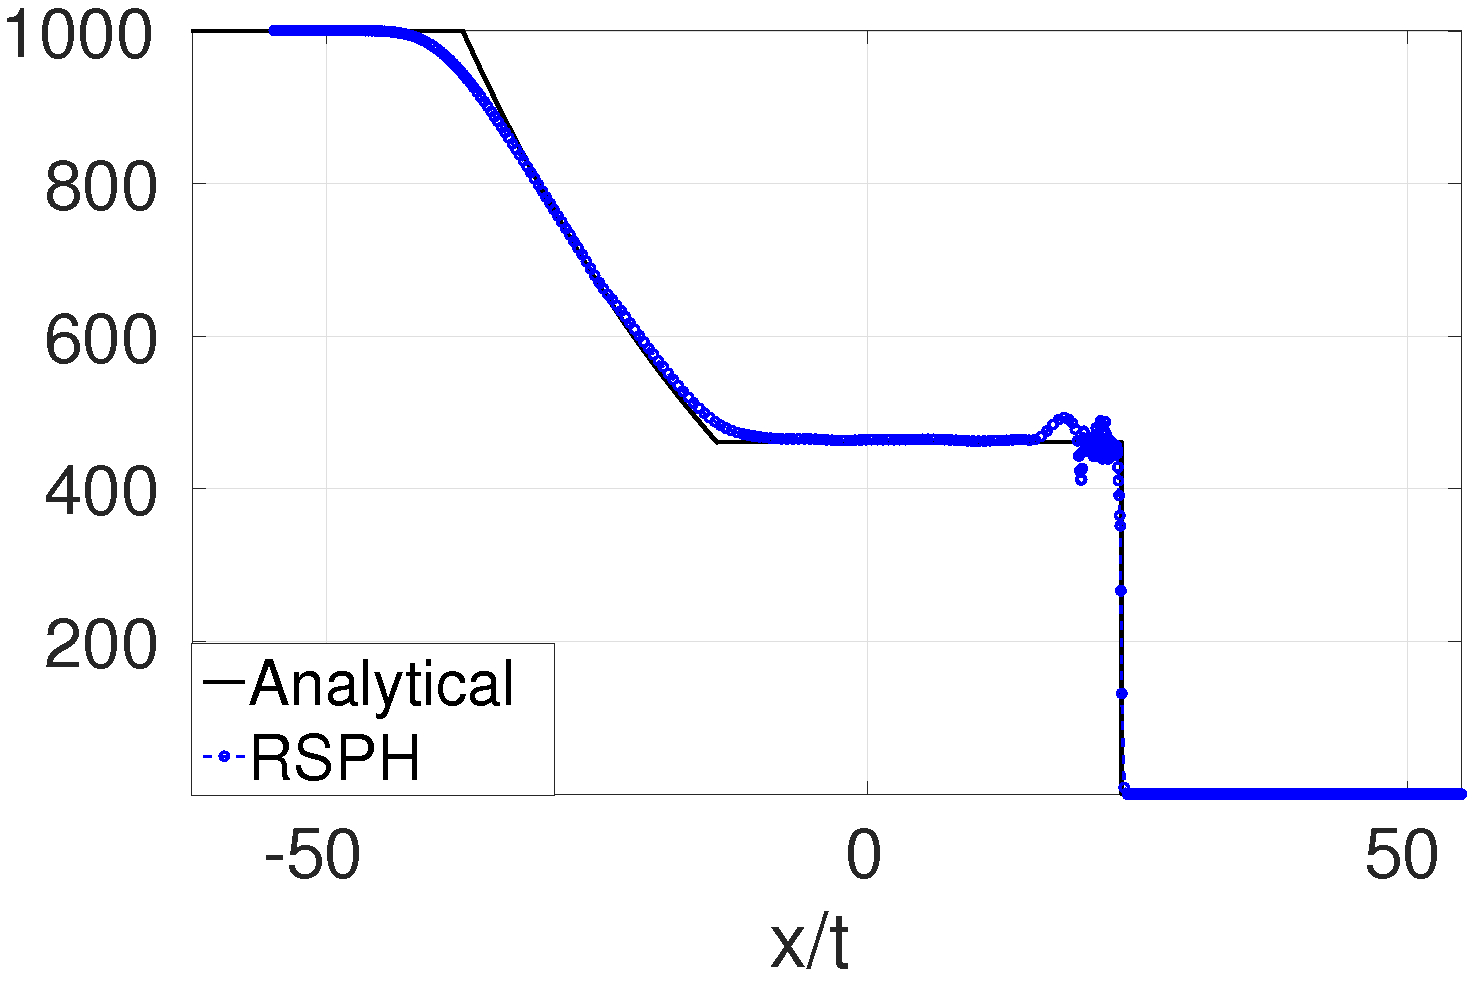
\includegraphics[width=0.99 \textwidth]{./Figures/StrBlst-RCM-p-Rp3}
    \end{minipage}% 
    \caption{Results for test 6, the strong blast test. y axis for density plot is in log base 10.  To stabilize the simulation, RSPH sampling is in a narrower range. All physical properties are well re-produced. The oscillations between shock and contact discontinuity is relatively larger than other area. A noticeable spike is observed near contact discontinuity.}
    \label{fig:RCM-strong-blast}
\end{figure}

\subsection{3D free jet} \label{jet}
Free jet flow have been studied analytically, experimentally and numerically for many decades, not only because of its wide application but also because of its fundamental significance as a basic flow to the scientific research community. To test the capacity of RSPH for multiple dimensional applications, a free jet flow is simulated in this section by solving 3D compressible Euler Equations using standard SPH, GSPH and RSPH. 
All simulations are using the same set-up and compared at the same physical time. Considering the fact that RSPH is based on piece wise constant construction of Riemann problem and a HLLC approximate Riemann solver, to do well-controlled comparisons, GSPH also adopts piece wise constant construction of Riemann problem and a HLLC Riemann solver. 

Setup of the 3D test is summarized briefly below. The computational domain is a box and boundaries are categorized into three types: the velocity inlet (a circular area at the center of the bottom of the box), the non-slip wall boundary (box bottom) and the pressure outlet (other faces of the box) boundary. At the vent, exit velocity $\textbf{v}$ is set to $500 m / s$ and radius of the nozzle $r$ is set to $8m $. The pressure of ejected fluid is assumed to be the same as ambient ($101 kpa$). The temperature of both ejected fluids and ambient fluids are set to $273 K$. 
Velocity is set to zero on the non-slip wall. The heat flux across wall boundary is also zero assuming an adiabatic wall. The flux of mass should be zero on the wall as well. As a result, internal energy flux, which consists of heat flux and energy flux carried by mass flux, vanishes on the non-slip wall boundary. 
The pressure of the surrounding ambient is given. As we ignore the physical viscosity, the shear stress is ignored and normal stress (whose magnitude equals to pressure) balances the ambient pressure.
\begin{equation}
p = p_a\left(z\right)  \label{eq:pressure_bc_p} 
\end{equation} 
Except for the pressure, boundary values for density, velocity, and energy on the outlet are dependent on solution. Fluids properties of ideal gas are used in this simulation.

\begin{figure}[H]
   \centering
   \includegraphics[width=0.95 \textwidth]{./Figures/SPH-3D-jet}
   \caption{Free jet flow simulation results at $t=3.0 s$ by SPH using different artificial viscosity coefficients. These pictures are front view of a slice of the domain cut by two planes parallel to $x-z$ plane at $y=-9$ and $y=9$. From left to right, the picture is corresponding to $\alpha=0.3$, $\alpha=1.0$ and $\alpha=2.0$ respectively. Another artificial viscosity coefficient $\beta$ is set to be double of $\alpha$ for all tests. Red particles in pictures are particles erupted from the nozzle while blues are ambient fluids particles. A positive correlation between overall damping effect and the distance from nozzle to the front of jet flow is shown.}
    \label{fig:free-jet-SPH-comparison}
\end{figure}

\begin{figure}[H]
    \centering
    \begin{minipage}[t]{.325 \textwidth}
        \centering
        \includegraphics[width=0.99 \textwidth]{./Figures/GSPH-HLLC-t1p5-cutView}
    \end{minipage}%
    \begin{minipage}[t]{.325\textwidth}
        \centering
        \includegraphics[width=0.99 \textwidth]{./Figures/RSPH-t1p5-cutView}
    \end{minipage}%
    \\
    \centering
    \begin{minipage}[t]{.325 \textwidth}
        \centering
        \includegraphics[width=0.99 \textwidth]{./Figures/GSPH-HLLC-t3-cutView}
    \end{minipage}%
    \begin{minipage}[t]{.325\textwidth}
        \centering
        \includegraphics[width=0.99 \textwidth]{./Figures/RSPH-t3-cutView}
    \end{minipage}%
    \caption{Simulation results of free jet flow by GSPH and RSPH. These pictures are front view of a slice of the domain cut by two planes parallel to $x-z$ plane at $y=-9$ and $y=9$. Pictures on the left side are for GSPH while those on the right side are for RSPH. Red particles in pictures are particles erupted from the nozzle while blues are ambient fluids particles. Pictures on the first row are corresponding to $t=1.5s$ while pictures on the second row are for $t=3.0 s$}
    \label{fig:free-jet-comparison}
\end{figure}

Figure \ref{fig:free-jet-SPH-comparison} shows simulation results of the free jet flow by SPH with different artificial viscosity coefficients. A positive correlation between overall damping effect (due to artificial dissipation) and the distance from nozzle to the front of jet flow is clearly shown in this figure. At $t=3.0 s$ after jet flow starting, we observe that the distances between the front of the jet flow and the nozzle increase when artificial viscosity coefficients decrease. The standard SPH adds artificial dissipation explicitly through the artificial viscosity term. The amount of artificial dissipation positively depends on artificial viscosity coefficients. In addition, there is no physical dissipation in the governing equations. So the numerical dissipation is the total dissipation. As shown in Fig. \ref{fig:free-jet-SPH-comparison}, the larger the artificial viscosity coefficients, the smaller the distance between the nozzle and the front of free jet flow. So the distance between nozzle and the front of free jet flow can be used as an indicator of equivalent numerical dissipation.
Our comparison between GSPH and RSPH in the next paragraph is based on the positive correlation between equivalent numerical dissipation and the distance from nozzle to the front of jet flow.

We compare RSPH with GSPH in terms of overall damping effects in Fig. \ref{fig:free-jet-comparison}. Different from SPH, both GSPH and RSPH introduce artificial viscosity in an implicit way by solving local Riemann problems. Based on the positive correlation between overall damping effect and the distance between the nozzle and the front of jet flow, we can infer the amount of equivalent numerical dissipation introduced by RSPH and GSPH. It has been shown in 1D tests that RSPH can introduce less artificial viscosity than GSPH. Fig. \ref{fig:free-jet-comparison} implies that RSPH introduces less overall damping effect than GSPH in 3D application as well, which is consistent with 1D tests. That is to say, RSPH's desirable property of introducing less artificial dissipation in 1D unsteady flow is inherited in 3D applications of RSPH. Recall that RCM shows ability of resolving discontinuities as true discontinuities in 1D unsteady flows but such very desirable property does not persist in genuine two (or higher) space dimensions \citep{colella1982glimm}. Integrating of RCM within the framework of SPH avoids solving higher dimensional Riemann problems overcoming the fundamental shortcoming of RCM.

\section{Conclusion} \label{discussion}
In this paper we have proposed RSPH, a novel SPH scheme for solving hyperbolic non-linear PDEs that combines the Random Choice Method with an approximate Riemann solver. No explicit artificial viscosity is needed. Instead, any viscosity that is used in a hydrodynamics simulation is just what the user implicitly adds. 
This control is important in applications with strong shocks. 
Unlike classical SPH which uses the same artificial viscosity coefficients everywhere, RSPH introduces larger dissipation around the shock to guarantee numerical stability while introduces much smaller dissipation elsewhere. Such adaptive manner of assigning dissipation reduces unnecessary numerical damping but preserves demanded damping for restraining numerical instability. As demonstrated in 1D and 3D tests, RSPH causes less smearing of shocks and less overall dissipation for jet flow.
In addition, RSPH also shows good convergence behavior.

On the other hand, RSPH does not address other methodological questions that must be decided in order to use SPH, questions such as the smoothing length of the SPH kernel. We have investigated the HLLC approximate Riemann solver in this paper; it is of interest to test other approximate solvers, to better understand the behavior of solutions. This may be particularly important when applying RSPH to other systems, where the explicit construction on which the HLLC solver rests is not readily available. In current implementation, the ``interface" between two particles are set at the middle. Alternative ways to determine the interface is also worthwhile to explore. 

\section*{Acknowledgements}
3D simulations reported here were performed at the Center for Computational Research (CCR) at the University at Buffalo. This project is supported by Grants No. NSF ACI/1131074 from the National Science Foundation. We want to give thanks to anonymous reviewers for their constructive comments.

\appendix
\section{Glimm\rq{}s Scheme}
In \citep{glimm1965solutions}, Glimm proved the existence  of solutions to a  $2\times2$ 
system of hyperbolic conservation laws within the space of total variation bounded functions. 
This proof constructed solutions in one space dimension (plus time) by solving local Riemann problems at `grid points\rq{}, sampling these local solutions randomly, and stitching them together to create the full solution.  Later \citet{liu1977deterministic} proved that a deterministic, uniform sampling 
method was sufficient to establish existence. \citet{chorin1976random} used
the random Glimm scheme as the basis of a numerical method to solve conservation laws, and
\citet{concus1979numerical} extended these ideas.
In his thesis, \citet{colella1978analysis} examined the van der Corput sequence as a sampling procedure (see also \cite{colella1982glimm}).

A signature feature of using Glimm\rq{}s method (or the random choice method) as a computational methodology is that
it introduces no artificial viscosity into the solution -- shocks and contact discontinuities are
resolved as sharp interfaces.  Let us explain by example. Consider a centered difference
method to solve the linear scalar equation 
\begin{equation}
\label{linear}
\frac{\partial u}{\partial t }+ a \frac{\partial u}{\partial x} = 0
\end{equation}
at cell index $j$ and time $n+1$:
\begin{equation}
u_j^{n+1} = u_j^n - a \frac{\Delta t}{\Delta x} \frac{(u_{j+1}^n - u_{j-1}^n)}{2}
\end{equation}
Of course this scheme is unconditionally unstable. Classical approaches to stabilizing the scheme add a small dose of artificial viscosity
\begin{equation}
u_j^{n+1} = u_j^n - a \frac{\Delta t}{\Delta x} \frac{(u_{j+1}^n - u_{j-1}^n)}{2} + a \frac{\Delta t}{2 \Delta x} (u_{j+1}^n -2 u_j^n + u_{j-1}^n)
\end{equation}
A stable first-order scheme such as upwind differencing (assuming $a>0$)
\begin{equation}
u_j^{n+1} = u_j^n - a \frac{\Delta t}{\Delta x} {(u_{j+1}^n - u_{j}^n)}
\end{equation}
can be seen as being second order accurate in space with a viscosity term added
\begin{equation}
u_j^{n+1} = u_j^n - a \frac{\Delta t}{\Delta x} \frac{(u_{j+1}^n - u_{j-1}^n)}{2} + a \frac{\Delta t}{2 \Delta x} (u_{j+1}^n -2 u_j^n + u_{j-1}^n))
\end{equation}
Examining dissipation effects for wide classes of finite difference/finite volume methods 
shows a similar phenomena (see, for example, \cite{warming1974modified}).

In contrast, Glimm\rq{}s approach solves a local Riemann problem exactly within each cell,
and samples (randomly or uniformly) the solution states. Consider again the linear advection equation \ref{linear}, with a discontinuity in cell $j$:
\begin{equation}
u^n = \begin{cases}
	u_L ~~~ x< (j+\xi)\Delta x \\
 	u_R ~~~ x> (j+\xi)\Delta x
	\end{cases}			
\end{equation}
where $0<\xi<1$ locates the discontinuity within cell $j$.

At time $n+1$, the discontinuity is either propagated or not, depending on the sampling
point:
\begin{equation}
u^{n+1} = \begin{cases}
		  u_L ~~~ x< (j+\tilde \xi)\Delta x + a \Delta t \\
		  u_R ~~~ x> (j+\tilde \xi)\Delta x + a \Delta t
	        \end{cases}
\end{equation}
where $\tilde \xi$ denotes the sample point.
In either case, the solution remains discontinuous at time $n+1$ and the 
discontinuity propagates at speed $a$ on average.

The random choice method requires an exact solution of every local Riemann problem, at every time step.
However this local solution is sampled, and much of the information present in the solution discarded.
Harten and Lax \citet{harten1981random} suggested solving the local Riemann problem approximately 
and sampling this approximate solution. The approximate solver reduces the computational
effort required in a numerical scheme, and the sampling recovers the zero viscosity
feature of the random choice method. \citet{hartenlax} suggest a finite difference
method as the approximate solver.
In our implementation, we propose the HLLC approximate solution as the foundation for
uniform sampling via the van der Corput sequence.
\citep{glimm1965solutions}
\citep{colella1982glimm}
\citep{chorin1976random}
\citep{concus1979numerical}
\citep{warming1974modified}
\citep{liu1977deterministic}

\section{Numerical oscillation due to non-uniform smoothing length in space}
Our discussion in this appendix is divided into two parts. The first part explains the mechanism how the numerical oscillations are induced by non-uniform smoothing length in space. The second parts  shows a ``manmade" numerical oscillation, which backs up our analysis in the first part.

There are several options \citep[][e.g.]{evrard1988beyond, hernquist1989treesph} for smoothing length $h$ in Eq. (\ref{eq:ns-sph-d} - \ref{eq:ns-sph-v}). Major discussions regarding the smoothing length are during 1980s to first several years of 1990s. In now days, taking $h=\frac{h_a + h_b}{2}$ is a commonly accepted practice. It is also adopted in this article. One big advantage is that such treatment can guarantee momentum and energy conservation given any paired particles are within compact support of each other's weighting function. However, it could also lead to numerical oscillation when applying the averaged smoothing length formulation in these scenarios with nonuniformly distributed smoothing length in space. Such numerical oscillation are usually either too small to observe or decays quickly due to sufficient (or too large) numerical dissipation. Such numerical oscillation is not fully aware of yet by the community. In this section we explain how the numerical oscillations are formed.

Recall that the kernel function of particle $a$ is required to be symmetric with respect to particle $a$. As a result, the gradient of kernel function at particle $a$ is anti-symmetric. All the commonly used kernel functions can satisfy the symmetry requirement as well as the anti-symmetry requirement of its gradient. The anti-symmetric properties of gradient of kernel function can guarantee the pressure gradient term, $\left(\dfrac{p_b}{\rho_b^2} + \dfrac{p_a}{\rho_a^2}\right) \nabla_a w_{a b}\left(h\right)$,  in momentum and energy equation (see Eq. (\ref{eq:ns-sph-v}) and (\ref{eq:ns-sph-e})), vanishes when pressure is uniform in space. For example, if pressure is uniform in space, pressure at particle $a$ and particle $b$ would be equal, the pressure gradient term then equals zero. That is, numerical approximation is consistent with real physics. However the actual kernel function is not symmetric any more if smoothing length is not uniform in space if we adopt the averaged smoothing length formulation. The gradient of kernel function is also not anti-symmetric any more. That is to say, the pressure gradient term becomes non-zero even when pressure is uniform in space. This unphysical representation of pressure gradient term by numerical approximation is illustrated in Fig. \ref{fig:dw-ha}. 

\begin{figure}[H]
\centering
\includegraphics[width=0.90 \textwidth ]{App-Figure/dw-ha}
\caption{In this example, we consider two pairs of particles $(a, b_1)$ and $(a, b_2)$. For simplicity, we assume uniform distance between particles. When take $h=\frac{h_a + h_b}{2}$, the actual shape of gradient of kernel function is the combination of two dash curves. It is not anti-symmetric.
We also assume pressure, density and particle mass of all particles are equal. However, the pressure gradient term at particle $a$ in discretized formulation do not cancel out ( $-\dfrac{p_{b_1}}{\rho_{b_1}^2} \nabla_a w_{a b_1}\left(\frac{h_a+h_{b_1}}{2}\right) < -\dfrac{p_{b_2}}{\rho_{b_2}^2} \nabla_a w_{a b2}\left(\frac{h_a+h_{b_1}}{2}\right)$) when smoothing lengths are not equal ($h_{b1} \neq h_{b2}$). This leads to unphysical non-zero pressure gradient, which is the source of numerical oscillation. When smoothing length is uniform in space or take $h = h_a$, the actual shape of gradient of kernel function is the solid curve, which is anti-symmetric. As a consequence, $-\dfrac{p_{b_1}}{\rho_{b_1}^2} \nabla_a w_{a b_1}\left(h\right) = \dfrac{p_{b_2}}{\rho_{b_2}^2} \nabla_a w_{a b2}\left(h\right)$, the unphysical non-zero pressure gradient vanishes.}    
\label{fig:dw-ha}
\end{figure}

To summarize, two necessary conditions for generating unphysical numerical representation of pressure gradient terms are:
\begin{itemize}
\item Calculate smoothing length by averaging, for example, $h = \frac{h_a + h_b}{2}$.
\item Smoothing length is nonuniform in space.
\end{itemize} 
This unphysical numerical representation of pressure gradient term could lead to numerical oscillation in numerical solution. Sharp changes in smoothing length can induce significant oscillation, which usually propagates into the computational domain and corrupts numerical solution.

To illustrate the formation and influence of such numerical oscillation, we intentionally create a situation of non-uniform smoothing length merely by assigning larger smoothing length to boundary ghost particles on left side in the 1D shock tube test (test2). As shown in the first plot of Fig. \ref{fig:Perturbation-ME2}, the smoothing length is discontinuous at the left boundary. \textbf{Just like discontinuity of physical quantities (for example, the discontinuity at the middle of shock tube test), discontinuity in numerical resolution, in terms of smoothing length, also induces a wave.} An oscillation is observed clearly in the simulation result, starting near the left boundary and propagating into simulation domain. Recall that larger smoothing length for left boundary ghost particles is the only difference between normal test (as shown in Fig. \ref{fig:RCM-GSPH-Sod}) and the new test (see Fig. \ref{fig:Perturbation-ME2}), we can conclude that nonuniform smoothing length in space do induce numerical oscillations.  Another important observation is that the magnitudes of oscillation decays as the time goes. We would suppose that it is due to numerical dissipation. In section \ref{sec:numericaltests}, we use magnitude of oscillation as an indirect indicator of numerical dissipation.

In another test, based on the previous test with larger smoothing length for ghost particle on left boundary, we adopt $h = h_a$, instead of $h = \frac{h_a + h_b}{2}$. The result is shown by Fig. \ref{fig:Perturbation-ME0-tp1}. The oscillation is gotten rid of, which confirms that the averaged smoothing length is one of necessary conditions for the unphysical numerical representation of pressure gradient term.
%Such perturbation would be created unintentionally in real implementation. The oscillation can actually be observed in 1D shock tube tests in many other papers, even though they are not as obvious as the one in Fig. \ref{fig:Perturbation-ME2}.

\begin{figure}[H]
\centering
\includegraphics[width=0.90 \textwidth]{App-Figure/Perturbation-ME2}
\caption{Plots of density for 1D shock tube test 2 at different time. The test is simulated using classical SPH with $\alpha = 1$. In these plots, $x$ axis is location along shock tube, $y$ axis is density. Smoothing length $h = \frac{h_a + h_b}{2}$. The first plot is corresponding to $t=0.001s$, color map is for smoothing length. The second plot to last plot are corresponding to $t=0.05s$, $t=0.1s$, $t=0.2s$, $t=0.3s$ respectively. We observe that a numerical perturbation incepts near the left boundary and propagates into the domain. Actually, the smoothing length is also discontinuous at the middle. It also induces another numerical perturbation which has smaller magnitude but still observable. It has the same propagating speed as the front of rarefaction. Both oscillations decays in time due to dissipation.}
\label{fig:Perturbation-ME2}
\end{figure}

\begin{figure}[H]
\centering
\includegraphics[width=0.90 \textwidth]{App-Figure/Perturbation-ME0-tp1}
\caption{Plots of density for 1D shock tube test 2 at $t=0.1s$. The test is simulated using classical SPH with $\alpha = 1$. In this test, we still intentionally create non-uniform smoothing length distribution in space by assigning larger smoothing length to boundary ghost particles at the left side. But we take $h=h_a$. No numerical perturbation generated near the left boundary.}    
\label{fig:Perturbation-ME0-tp1}
\end{figure}

Adaptive smoothing length is now an essential component of SPH method. It naturely results to nonuniform smoothing length in space. Variation range of smoothing length would be especially larger for compressible flow. Fortunately, there are several factors counteracting against the numerical oscillation:
\begin{itemize}
\item Numerical dissipation decays such numerical oscillation preventing accumulation of oscillation magnitude.
\item For incompressible flow or weakly compressible flow, smoothing length only varies in a small range.
\item Well developed adaptive smoothing length algorithm usually guarantees more ``smoothing" change of smoothing length in space avoiding sharp change of smoothing length in space.
\end{itemize}
So we do not think that the numerical oscillation is a challenging issue for SPH. The major motivation of the appendix is to show that 
\begin{itemize}
\item The numerical oscillation does exist commonly in SPH schemes. It is not something only for RSPH.
\item Dissipation decays the oscillation, so numerical oscillation can serve as an indicator of dissipation.
\end{itemize}
\section*{References}
 \bibliographystyle{elsarticle-num} 
\bibliography{Reference}

\end{document}
